% Options for packages loaded elsewhere
\PassOptionsToPackage{unicode}{hyperref}
\PassOptionsToPackage{hyphens}{url}
%
\documentclass[
  ignorenonframetext,
]{beamer}
\usepackage{pgfpages}
\setbeamertemplate{caption}[numbered]
\setbeamertemplate{caption label separator}{: }
\setbeamercolor{caption name}{fg=normal text.fg}
\beamertemplatenavigationsymbolsempty
% Prevent slide breaks in the middle of a paragraph
\widowpenalties 1 10000
\raggedbottom
\setbeamertemplate{part page}{
  \centering
  \begin{beamercolorbox}[sep=16pt,center]{part title}
    \usebeamerfont{part title}\insertpart\par
  \end{beamercolorbox}
}
\setbeamertemplate{section page}{
  \centering
  \begin{beamercolorbox}[sep=12pt,center]{part title}
    \usebeamerfont{section title}\insertsection\par
  \end{beamercolorbox}
}
\setbeamertemplate{subsection page}{
  \centering
  \begin{beamercolorbox}[sep=8pt,center]{part title}
    \usebeamerfont{subsection title}\insertsubsection\par
  \end{beamercolorbox}
}
\AtBeginPart{
  \frame{\partpage}
}
\AtBeginSection{
  \ifbibliography
  \else
    \frame{\sectionpage}
  \fi
}
\AtBeginSubsection{
  \frame{\subsectionpage}
}
\usepackage{amsmath,amssymb}
\usepackage{iftex}
\ifPDFTeX
  \usepackage[T1]{fontenc}
  \usepackage[utf8]{inputenc}
  \usepackage{textcomp} % provide euro and other symbols
\else % if luatex or xetex
  \usepackage{unicode-math} % this also loads fontspec
  \defaultfontfeatures{Scale=MatchLowercase}
  \defaultfontfeatures[\rmfamily]{Ligatures=TeX,Scale=1}
\fi
\usepackage{lmodern}
\usetheme[]{Madrid}
\usecolortheme{orchid}
\usefonttheme{professionalfonts}
\ifPDFTeX\else
  % xetex/luatex font selection
\fi
% Use upquote if available, for straight quotes in verbatim environments
\IfFileExists{upquote.sty}{\usepackage{upquote}}{}
\IfFileExists{microtype.sty}{% use microtype if available
  \usepackage[]{microtype}
  \UseMicrotypeSet[protrusion]{basicmath} % disable protrusion for tt fonts
}{}
\makeatletter
\@ifundefined{KOMAClassName}{% if non-KOMA class
  \IfFileExists{parskip.sty}{%
    \usepackage{parskip}
  }{% else
    \setlength{\parindent}{0pt}
    \setlength{\parskip}{6pt plus 2pt minus 1pt}}
}{% if KOMA class
  \KOMAoptions{parskip=half}}
\makeatother
\usepackage{xcolor}
\newif\ifbibliography
\usepackage{color}
\usepackage{fancyvrb}
\newcommand{\VerbBar}{|}
\newcommand{\VERB}{\Verb[commandchars=\\\{\}]}
\DefineVerbatimEnvironment{Highlighting}{Verbatim}{commandchars=\\\{\}}
% Add ',fontsize=\small' for more characters per line
\usepackage{framed}
\definecolor{shadecolor}{RGB}{248,248,248}
\newenvironment{Shaded}{\begin{snugshade}}{\end{snugshade}}
\newcommand{\AlertTok}[1]{\textcolor[rgb]{0.94,0.16,0.16}{#1}}
\newcommand{\AnnotationTok}[1]{\textcolor[rgb]{0.56,0.35,0.01}{\textbf{\textit{#1}}}}
\newcommand{\AttributeTok}[1]{\textcolor[rgb]{0.13,0.29,0.53}{#1}}
\newcommand{\BaseNTok}[1]{\textcolor[rgb]{0.00,0.00,0.81}{#1}}
\newcommand{\BuiltInTok}[1]{#1}
\newcommand{\CharTok}[1]{\textcolor[rgb]{0.31,0.60,0.02}{#1}}
\newcommand{\CommentTok}[1]{\textcolor[rgb]{0.56,0.35,0.01}{\textit{#1}}}
\newcommand{\CommentVarTok}[1]{\textcolor[rgb]{0.56,0.35,0.01}{\textbf{\textit{#1}}}}
\newcommand{\ConstantTok}[1]{\textcolor[rgb]{0.56,0.35,0.01}{#1}}
\newcommand{\ControlFlowTok}[1]{\textcolor[rgb]{0.13,0.29,0.53}{\textbf{#1}}}
\newcommand{\DataTypeTok}[1]{\textcolor[rgb]{0.13,0.29,0.53}{#1}}
\newcommand{\DecValTok}[1]{\textcolor[rgb]{0.00,0.00,0.81}{#1}}
\newcommand{\DocumentationTok}[1]{\textcolor[rgb]{0.56,0.35,0.01}{\textbf{\textit{#1}}}}
\newcommand{\ErrorTok}[1]{\textcolor[rgb]{0.64,0.00,0.00}{\textbf{#1}}}
\newcommand{\ExtensionTok}[1]{#1}
\newcommand{\FloatTok}[1]{\textcolor[rgb]{0.00,0.00,0.81}{#1}}
\newcommand{\FunctionTok}[1]{\textcolor[rgb]{0.13,0.29,0.53}{\textbf{#1}}}
\newcommand{\ImportTok}[1]{#1}
\newcommand{\InformationTok}[1]{\textcolor[rgb]{0.56,0.35,0.01}{\textbf{\textit{#1}}}}
\newcommand{\KeywordTok}[1]{\textcolor[rgb]{0.13,0.29,0.53}{\textbf{#1}}}
\newcommand{\NormalTok}[1]{#1}
\newcommand{\OperatorTok}[1]{\textcolor[rgb]{0.81,0.36,0.00}{\textbf{#1}}}
\newcommand{\OtherTok}[1]{\textcolor[rgb]{0.56,0.35,0.01}{#1}}
\newcommand{\PreprocessorTok}[1]{\textcolor[rgb]{0.56,0.35,0.01}{\textit{#1}}}
\newcommand{\RegionMarkerTok}[1]{#1}
\newcommand{\SpecialCharTok}[1]{\textcolor[rgb]{0.81,0.36,0.00}{\textbf{#1}}}
\newcommand{\SpecialStringTok}[1]{\textcolor[rgb]{0.31,0.60,0.02}{#1}}
\newcommand{\StringTok}[1]{\textcolor[rgb]{0.31,0.60,0.02}{#1}}
\newcommand{\VariableTok}[1]{\textcolor[rgb]{0.00,0.00,0.00}{#1}}
\newcommand{\VerbatimStringTok}[1]{\textcolor[rgb]{0.31,0.60,0.02}{#1}}
\newcommand{\WarningTok}[1]{\textcolor[rgb]{0.56,0.35,0.01}{\textbf{\textit{#1}}}}
\setlength{\emergencystretch}{3em} % prevent overfull lines
\providecommand{\tightlist}{%
  \setlength{\itemsep}{0pt}\setlength{\parskip}{0pt}}
\setcounter{secnumdepth}{-\maxdimen} % remove section numbering
\usepackage{placeins}
\usepackage{color}
\usepackage{bm}
\usepackage{amsmath}
\usepackage{algorithm}
\usepackage[]{algpseudocode}
\usepackage{tabularx}
\usepackage{multirow}
\usepackage[most]{tcolorbox}
\usepackage{tikz}
\usepackage{lipsum}
\usepackage{mathtools}
\usepackage{actuarialangle}
\usepackage{multirow, longtable, array, dcolumn}
\usepackage{tabu}
\newcommand{\sdt}{\bullet}
\newcommand{\tss}{\textsuperscript}
\newcommand{\morearraysp}{\setlength{\arraycolsep}{2mm}}
\newcommand{\smarraysp}{\setlength{\arraycolsep}{1mm}}
\newcommand{\oldarraysp}{\setlength{\arraycolsep}{1.5pt}}
\newcommand{\matrixstretch}{\setlength{\extrarowheight}{4pt}}
\newcommand{\matrixnostretch}{\setlength{\extrarowheight}{0pt}}
\newcommand{\gil}[1]{\textrm{\gilfont{#1}}\normalfont }
\newfont{\gilfont}{msbm10 scaled 1000}
\newcommand{\DOT}{\usebox{\biggercirc}}
\newcommand{\pv}{\wp\text{-value}}
\ifLuaTeX
  \usepackage{selnolig}  % disable illegal ligatures
\fi
\IfFileExists{bookmark.sty}{\usepackage{bookmark}}{\usepackage{hyperref}}
\IfFileExists{xurl.sty}{\usepackage{xurl}}{} % add URL line breaks if available
\urlstyle{same}
\hypersetup{
  pdftitle={STT 3850 : Week 10},
  pdfauthor={Spring 2024},
  hidelinks,
  pdfcreator={LaTeX via pandoc}}

\title{STT 3850 : Week 10}
\author{Spring 2024}
\date{}
\institute{Appalachian State University}

\begin{document}
\frame{\titlepage}

\hypertarget{outline-for-the-week}{%
\section{Outline for the week}\label{outline-for-the-week}}

\begin{frame}{By the end of the week: Bootstrapping and Confidence
Intervals}
\protect\hypertarget{by-the-end-of-the-week-bootstrapping-and-confidence-intervals}{}
\begin{itemize}
\item
  Key features of the Bootstrap and understanding confidence intervals
\item
  Constructing and interpreting confidence intervals
\item
  Two sample bootstrap
\item
  Theory-based confidence intervals (mean (sigma known) , mean (sigma
  unknown), assumptions underlying t-confidence interval)
\end{itemize}
\end{frame}

\hypertarget{key-features-of-the-bootstrap}{%
\section{Key features of the
Bootstrap}\label{key-features-of-the-bootstrap}}

\begin{frame}[fragile]{Needed packages}
\protect\hypertarget{needed-packages}{}
\small

\begin{Shaded}
\begin{Highlighting}[]
\FunctionTok{library}\NormalTok{(tidyverse)}
\FunctionTok{library}\NormalTok{(moderndive)}
\FunctionTok{library}\NormalTok{(infer)}
\FunctionTok{library}\NormalTok{(resampledata)}
\end{Highlighting}
\end{Shaded}

\normalsize
\end{frame}

\begin{frame}{Key features of the Bootstrap: Example 1}
\protect\hypertarget{key-features-of-the-bootstrap-example-1}{}
To highlight some key features of the bootstrap distribution:

\begin{itemize}
\item
  Consider two examples in which the theoretical sampling distributions
  of the mean are known.
\item
  Example 1: Consider a random sample of size 49 drawn from a
  \(N(25, 7)\).

  \begin{itemize}
  \tightlist
  \item
    Theory tells us that that the sampling distribution of the sample
    means is normal with mean 25 and standard error
    \(\sigma_{\bar{x}}=7/\sqrt{49}=1\).
  \end{itemize}
\end{itemize}
\end{frame}

\begin{frame}[fragile]{Key features of the Bootstrap: Example 1}
\protect\hypertarget{key-features-of-the-bootstrap-example-1-1}{}
\tiny

\begin{Shaded}
\begin{Highlighting}[]
\FunctionTok{set.seed}\NormalTok{(}\DecValTok{11}\NormalTok{)}
\FunctionTok{par}\NormalTok{(}\AttributeTok{mfrow =} \FunctionTok{c}\NormalTok{(}\DecValTok{3}\NormalTok{, }\DecValTok{2}\NormalTok{))}
\FunctionTok{curve}\NormalTok{(}\FunctionTok{dnorm}\NormalTok{(x, }\DecValTok{25}\NormalTok{, }\DecValTok{7}\NormalTok{), }\AttributeTok{from =} \DecValTok{25} \SpecialCharTok{{-}} \FloatTok{2.5}\SpecialCharTok{*}\DecValTok{7}\NormalTok{, }\DecValTok{25} \SpecialCharTok{+} \FloatTok{2.5}\SpecialCharTok{*}\DecValTok{7}\NormalTok{, }\AttributeTok{col =} \StringTok{"blue"}\NormalTok{, }\AttributeTok{main =} \StringTok{"N(25, 7)"}\NormalTok{, }\AttributeTok{ylab =} \StringTok{""}\NormalTok{, }\AttributeTok{xlab =} \StringTok{""}\NormalTok{)}
\FunctionTok{abline}\NormalTok{(}\AttributeTok{v =} \DecValTok{25}\NormalTok{, }\AttributeTok{col =} \StringTok{"red"}\NormalTok{)}
\FunctionTok{curve}\NormalTok{(}\FunctionTok{dnorm}\NormalTok{(x, }\DecValTok{25}\NormalTok{, }\DecValTok{1}\NormalTok{), }\AttributeTok{from =} \DecValTok{25} \SpecialCharTok{{-}} \FloatTok{2.5}\SpecialCharTok{*}\DecValTok{7}\NormalTok{, }\DecValTok{25} \SpecialCharTok{+} \FloatTok{2.5}\SpecialCharTok{*}\DecValTok{7}\NormalTok{, }\AttributeTok{col =} \StringTok{"blue"}\NormalTok{, }\AttributeTok{main =} \StringTok{"N(25, 1)"}\NormalTok{, }\AttributeTok{ylab =} \StringTok{""}\NormalTok{, }\AttributeTok{xlab =} \StringTok{""}\NormalTok{)}
\FunctionTok{abline}\NormalTok{(}\AttributeTok{v =} \DecValTok{25}\NormalTok{, }\AttributeTok{col =} \StringTok{"red"}\NormalTok{)}
\NormalTok{rs1 }\OtherTok{\textless{}{-}} \FunctionTok{rnorm}\NormalTok{(}\DecValTok{49}\NormalTok{, }\DecValTok{25}\NormalTok{, }\DecValTok{7}\NormalTok{)}
\NormalTok{rs2 }\OtherTok{\textless{}{-}} \FunctionTok{rnorm}\NormalTok{(}\DecValTok{49}\NormalTok{, }\DecValTok{25}\NormalTok{, }\DecValTok{7}\NormalTok{)}
\FunctionTok{hist}\NormalTok{(rs1, }\AttributeTok{xlab =} \StringTok{""}\NormalTok{, }\AttributeTok{main =} \StringTok{"n = 49"}\NormalTok{)}
\FunctionTok{abline}\NormalTok{(}\AttributeTok{v =} \FunctionTok{mean}\NormalTok{(rs1), }\AttributeTok{col =} \StringTok{"red"}\NormalTok{)}
\NormalTok{B }\OtherTok{\textless{}{-}} \DecValTok{10000}
\NormalTok{my.boot.stat1 }\OtherTok{\textless{}{-}} \FunctionTok{numeric}\NormalTok{(B)}
\NormalTok{my.boot.stat2 }\OtherTok{\textless{}{-}} \FunctionTok{numeric}\NormalTok{(B)}
\ControlFlowTok{for}\NormalTok{ (i }\ControlFlowTok{in} \DecValTok{1}\SpecialCharTok{:}\NormalTok{B)\{}
\NormalTok{  x1 }\OtherTok{\textless{}{-}} \FunctionTok{sample}\NormalTok{(rs1, }\AttributeTok{size =} \DecValTok{49}\NormalTok{, }\AttributeTok{replace =} \ConstantTok{TRUE}\NormalTok{) }
\NormalTok{  x2 }\OtherTok{\textless{}{-}} \FunctionTok{sample}\NormalTok{(rs2, }\AttributeTok{size =} \DecValTok{49}\NormalTok{, }\AttributeTok{replace =} \ConstantTok{TRUE}\NormalTok{) }
\NormalTok{  my.boot.stat1[i] }\OtherTok{\textless{}{-}} \FunctionTok{mean}\NormalTok{(x1)}
\NormalTok{  my.boot.stat2[i] }\OtherTok{\textless{}{-}} \FunctionTok{mean}\NormalTok{(x2)}
\NormalTok{\}}
\FunctionTok{hist}\NormalTok{(my.boot.stat1, }\AttributeTok{breaks =} \StringTok{"Scott"}\NormalTok{,  }\AttributeTok{main =}\StringTok{"Bootstrap Distribution"}\NormalTok{, }\AttributeTok{freq=} \ConstantTok{FALSE}\NormalTok{, }\AttributeTok{xlab =} \StringTok{""}\NormalTok{, }
\AttributeTok{xlim =} \FunctionTok{c}\NormalTok{(}\DecValTok{25} \SpecialCharTok{{-}} \FloatTok{2.5}\SpecialCharTok{*}\DecValTok{7}\NormalTok{, }\DecValTok{25} \SpecialCharTok{+} \FloatTok{2.5}\SpecialCharTok{*}\DecValTok{7}\NormalTok{))}
\FunctionTok{abline}\NormalTok{(}\AttributeTok{v =} \FunctionTok{mean}\NormalTok{(rs1), }\AttributeTok{col =} \StringTok{"red"}\NormalTok{)}
\FunctionTok{hist}\NormalTok{(rs2, }\AttributeTok{xlab =} \StringTok{""}\NormalTok{, }\AttributeTok{main =} \StringTok{"n = 49"}\NormalTok{)}
\FunctionTok{abline}\NormalTok{(}\AttributeTok{v =} \FunctionTok{mean}\NormalTok{(rs2), }\AttributeTok{col =} \StringTok{"red"}\NormalTok{)}
\FunctionTok{hist}\NormalTok{(my.boot.stat2, }\AttributeTok{breaks =} \StringTok{"Scott"}\NormalTok{,  }\AttributeTok{main =}\StringTok{"Bootstrap Distribution"}\NormalTok{, }\AttributeTok{freq=} \ConstantTok{FALSE}\NormalTok{, }\AttributeTok{xlab =} \StringTok{""}\NormalTok{, }
\AttributeTok{xlim =} \FunctionTok{c}\NormalTok{(}\DecValTok{25} \SpecialCharTok{{-}} \FloatTok{2.5}\SpecialCharTok{*}\DecValTok{7}\NormalTok{, }\DecValTok{25} \SpecialCharTok{+} \FloatTok{2.5}\SpecialCharTok{*}\DecValTok{7}\NormalTok{))}
\FunctionTok{abline}\NormalTok{(}\AttributeTok{v =} \FunctionTok{mean}\NormalTok{(rs2), }\AttributeTok{col =} \StringTok{"red"}\NormalTok{)}
\FunctionTok{c}\NormalTok{(}\FunctionTok{mean}\NormalTok{(rs1), }\FunctionTok{sd}\NormalTok{(rs1), }\FunctionTok{mean}\NormalTok{(rs2), }\FunctionTok{sd}\NormalTok{(rs2), }
  \FunctionTok{mean}\NormalTok{(my.boot.stat1), }\FunctionTok{sd}\NormalTok{(my.boot.stat1), }\FunctionTok{mean}\NormalTok{(my.boot.stat2), }\FunctionTok{sd}\NormalTok{(my.boot.stat2))}
\end{Highlighting}
\end{Shaded}

\normalsize
\end{frame}

\begin{frame}[fragile]{Key features of the Bootstrap: Example 1}
\protect\hypertarget{key-features-of-the-bootstrap-example-1-2}{}
\tiny

\begin{center}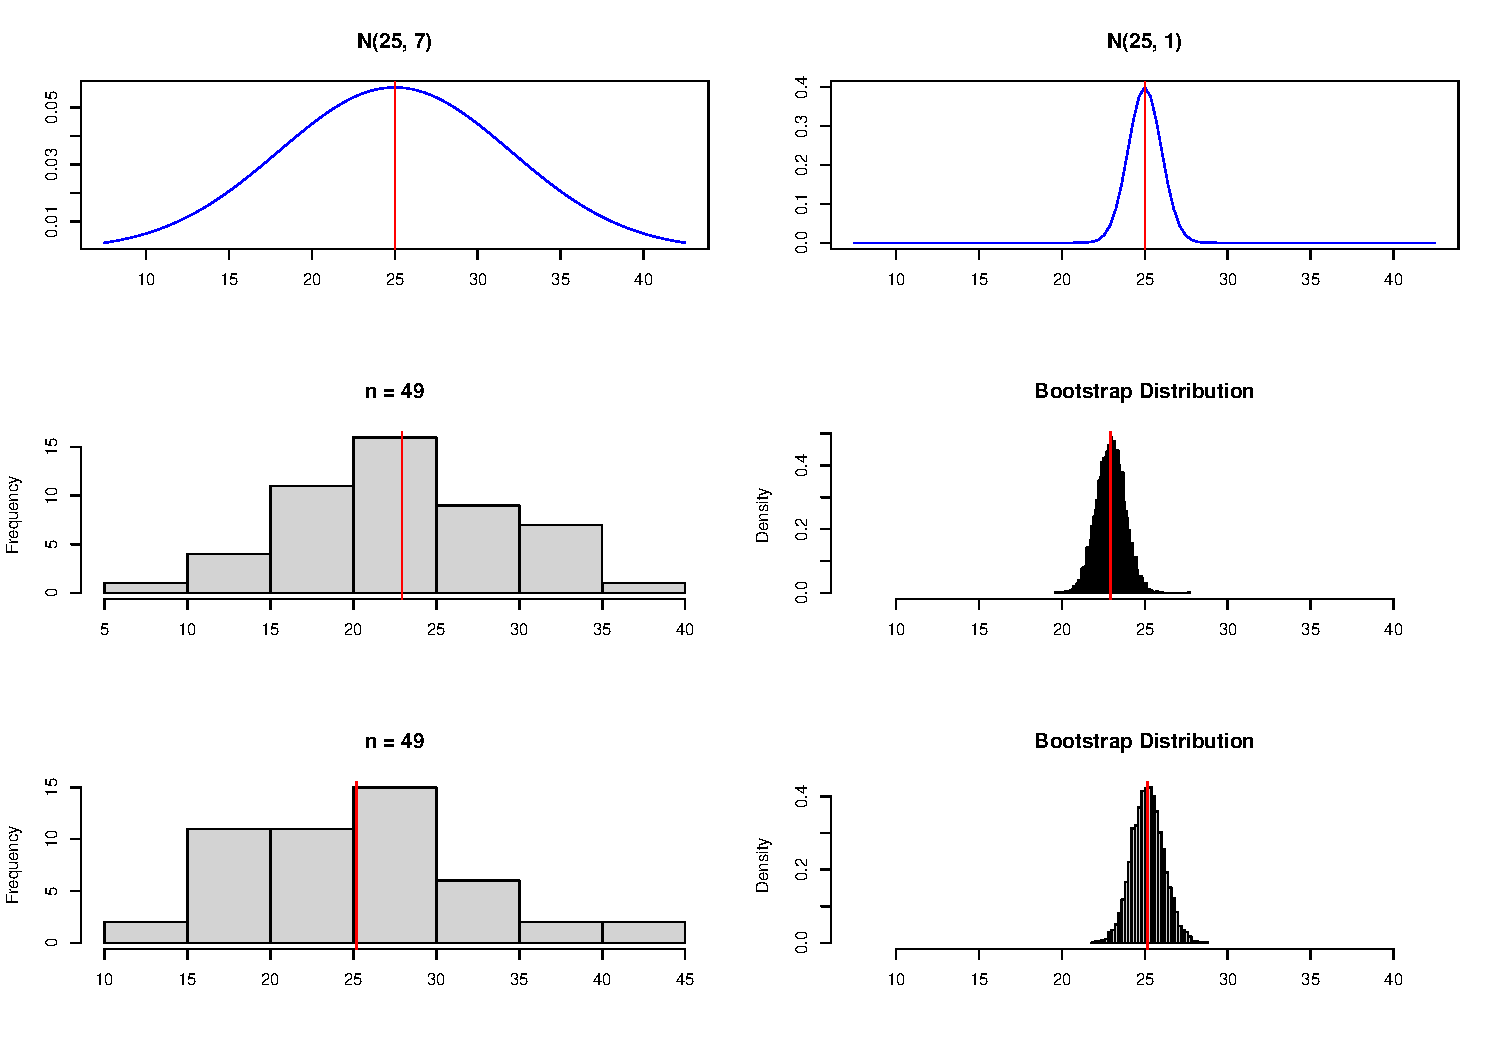
\includegraphics[width=0.9\linewidth,height=0.75\textheight]{Week10_Lect_files/figure-beamer/unnamed-chunk-3-1} \end{center}

\begin{verbatim}
[1] 22.9402808  5.9322341 25.1793901  6.6413206 22.9464693  0.8458991 25.1774556
[8]  0.9419660
\end{verbatim}

\normalsize
\end{frame}

\begin{frame}{Key features of the Bootstrap: Example 1}
\protect\hypertarget{key-features-of-the-bootstrap-example-1-3}{}
\begin{itemize}
\item
  The previous code shows the distributions of two such random samples
  with sample means:

  \begin{itemize}
  \tightlist
  \item
    \(\bar{x}_1=22.9402808\) and, \(\bar{x}_2=25.1793901\)
  \item
    \(s_1= 5.9322341\) and, \(s_2= 6.6413206\)
  \end{itemize}
\item
  Based on the graphs above, we can see that the bootstrap distribution:

  \begin{itemize}
  \tightlist
  \item
    has roughly the same spread and shape as the theoretical sampling
    distribution,
  \item
    but the centers are different compared to the theoretical sampling
    distribution.
  \end{itemize}
\end{itemize}
\end{frame}

\begin{frame}{Key features of the Bootstrap: Example 1}
\protect\hypertarget{key-features-of-the-bootstrap-example-1-4}{}
\begin{itemize}
\item
  This example illustrates some important features of the bootstrap that
  hold for other statistics besides the mean:

  \begin{itemize}
  \tightlist
  \item
    the bootstrap distribution of a particular statistic
    \(\hat{\theta}\) has approximately the same spread and shape as the
    sampling distribution of the statistic \(\hat{\theta}\), but
  \item
    the center of the bootstrap distribution is at the center of the
    original sample.
  \end{itemize}
\item
  Hence we do not use the center of the bootstrap distribution in its
  own right, but we do compare the center of the bootstrap distribution
  with the observed statistic; if they differ, it indicates bias.
\item
  For most statistics, bootstrap distributions approximate the spread,
  bias, and shape of the actual sampling distribution.
\end{itemize}
\end{frame}

\begin{frame}{Key features of the Bootstrap: Example 2}
\protect\hypertarget{key-features-of-the-bootstrap-example-2}{}
We now consider an example where neither the population nor the sampling
distribution is normal.

\begin{itemize}
\item
  A random variable \(X\) that has a Gamma distribution is written
  \(X\sim \Gamma(\alpha, \lambda)\).
\item
  If \(X\) is a Gamma random variable, then:
  \[E[X]=\alpha/\lambda \quad \quad \text{and} \quad \quad Var[X]=\alpha/\lambda^2.\]
\item
  Let \(X_1, \ldots, X_n\sim \Gamma(\alpha = 1, \lambda = 1/2)\).

  \begin{itemize}
  \tightlist
  \item
    It is a fact that the sampling distribution of the mean \(\bar{X}\)
    is \(\Gamma(n\alpha = 16\cdot 1 = 16, n\lambda = 16/2 = 8)\).
  \end{itemize}
\item
  We draw a random sample of size \(n=16\) from a
  \(\Gamma(\alpha=1, \lambda=1/2)\) (population mean:
  \(\alpha/\lambda= 2\), standard deviation:
  \(\sqrt{\alpha/\lambda^2 = 1/(1/2)^2)}=2\)).
\end{itemize}
\end{frame}

\begin{frame}[fragile]{Key features of the Bootstrap: Example 2}
\protect\hypertarget{key-features-of-the-bootstrap-example-2-1}{}
\tiny

\begin{Shaded}
\begin{Highlighting}[]
\FunctionTok{set.seed}\NormalTok{(}\DecValTok{281}\NormalTok{)}
\FunctionTok{par}\NormalTok{(}\AttributeTok{mfrow =} \FunctionTok{c}\NormalTok{(}\DecValTok{3}\NormalTok{, }\DecValTok{2}\NormalTok{))}
\FunctionTok{curve}\NormalTok{(}\FunctionTok{dgamma}\NormalTok{(x, }\DecValTok{1}\NormalTok{, }\DecValTok{1}\SpecialCharTok{/}\DecValTok{2}\NormalTok{), }\AttributeTok{from =} \DecValTok{0}\NormalTok{, }\AttributeTok{to =} \DecValTok{8}\NormalTok{, }\AttributeTok{col =} \StringTok{"blue"}\NormalTok{, }\AttributeTok{main =} \StringTok{"Gamma(1, 1/2)"}\NormalTok{, }\AttributeTok{ylab =} \StringTok{""}\NormalTok{, }\AttributeTok{xlab =} \StringTok{""}\NormalTok{)}
\FunctionTok{abline}\NormalTok{(}\AttributeTok{v =} \DecValTok{2}\NormalTok{, }\AttributeTok{col =} \StringTok{"red"}\NormalTok{)}
\FunctionTok{curve}\NormalTok{(}\FunctionTok{dgamma}\NormalTok{(x, }\DecValTok{16}\NormalTok{, }\DecValTok{8}\NormalTok{), }\AttributeTok{from =} \DecValTok{0}\NormalTok{, }\DecValTok{8}\NormalTok{, }\AttributeTok{col =} \StringTok{"blue"}\NormalTok{, }\AttributeTok{main =} \StringTok{"Gamma(16, 8)"}\NormalTok{, }\AttributeTok{ylab =} \StringTok{""}\NormalTok{, }\AttributeTok{xlab =} \StringTok{""}\NormalTok{)}
\FunctionTok{abline}\NormalTok{(}\AttributeTok{v =} \DecValTok{2}\NormalTok{, }\AttributeTok{col =} \StringTok{"red"}\NormalTok{)}
\NormalTok{rsg1 }\OtherTok{\textless{}{-}} \FunctionTok{rgamma}\NormalTok{(}\DecValTok{16}\NormalTok{, }\DecValTok{1}\NormalTok{, }\DecValTok{1}\SpecialCharTok{/}\DecValTok{2}\NormalTok{)}
\NormalTok{rsg2 }\OtherTok{\textless{}{-}} \FunctionTok{rgamma}\NormalTok{(}\DecValTok{16}\NormalTok{, }\DecValTok{1}\NormalTok{, }\DecValTok{1}\SpecialCharTok{/}\DecValTok{2}\NormalTok{)}
\FunctionTok{hist}\NormalTok{(rsg1, }\AttributeTok{xlab =} \StringTok{""}\NormalTok{, }\AttributeTok{main =} \StringTok{"n = 16"}\NormalTok{, }\AttributeTok{xlim =} \FunctionTok{c}\NormalTok{(}\DecValTok{0}\NormalTok{, }\DecValTok{8}\NormalTok{))}
\FunctionTok{abline}\NormalTok{(}\AttributeTok{v =} \FunctionTok{mean}\NormalTok{(rsg1), }\AttributeTok{col =} \StringTok{"red"}\NormalTok{)}
\NormalTok{B }\OtherTok{\textless{}{-}} \DecValTok{10000}
\NormalTok{my.boot.statg1 }\OtherTok{\textless{}{-}} \FunctionTok{numeric}\NormalTok{(B)}
\NormalTok{my.boot.statg2 }\OtherTok{\textless{}{-}} \FunctionTok{numeric}\NormalTok{(B)}
\ControlFlowTok{for}\NormalTok{ (i }\ControlFlowTok{in} \DecValTok{1}\SpecialCharTok{:}\NormalTok{B)\{}
\NormalTok{  xg1 }\OtherTok{\textless{}{-}} \FunctionTok{sample}\NormalTok{(rsg1, }\AttributeTok{size =} \DecValTok{16}\NormalTok{, }\AttributeTok{replace =} \ConstantTok{TRUE}\NormalTok{)}
\NormalTok{  xg2 }\OtherTok{\textless{}{-}} \FunctionTok{sample}\NormalTok{(rsg2, }\AttributeTok{size =} \DecValTok{16}\NormalTok{, }\AttributeTok{replace =} \ConstantTok{TRUE}\NormalTok{)}
\NormalTok{  my.boot.statg1[i] }\OtherTok{\textless{}{-}} \FunctionTok{mean}\NormalTok{(xg1)}
\NormalTok{  my.boot.statg2[i] }\OtherTok{\textless{}{-}} \FunctionTok{mean}\NormalTok{(xg2)}
\NormalTok{\}}
\FunctionTok{hist}\NormalTok{(my.boot.statg1, }\AttributeTok{breaks =} \StringTok{"Scott"}\NormalTok{,  }\AttributeTok{main =}\StringTok{"Bootstrap Distribution"}\NormalTok{, }\AttributeTok{freq=} \ConstantTok{FALSE}\NormalTok{, }\AttributeTok{xlab =} \StringTok{""}\NormalTok{, }
\AttributeTok{xlim =} \FunctionTok{c}\NormalTok{(}\DecValTok{0}\NormalTok{, }\DecValTok{8}\NormalTok{))}
\FunctionTok{abline}\NormalTok{(}\AttributeTok{v =} \FunctionTok{mean}\NormalTok{(rsg1), }\AttributeTok{col =} \StringTok{"red"}\NormalTok{)}
\FunctionTok{hist}\NormalTok{(rsg2, }\AttributeTok{xlab =} \StringTok{""}\NormalTok{, }\AttributeTok{main =} \StringTok{"n = 16"}\NormalTok{, }\AttributeTok{xlim =} \FunctionTok{c}\NormalTok{(}\DecValTok{0}\NormalTok{, }\DecValTok{8}\NormalTok{))}
\FunctionTok{abline}\NormalTok{(}\AttributeTok{v =} \FunctionTok{mean}\NormalTok{(rsg2), }\AttributeTok{col =} \StringTok{"red"}\NormalTok{)}
\FunctionTok{hist}\NormalTok{(my.boot.statg2, }\AttributeTok{breaks =} \StringTok{"Scott"}\NormalTok{,  }\AttributeTok{main =}\StringTok{"Bootstrap Distribution"}\NormalTok{, }\AttributeTok{freq=} \ConstantTok{FALSE}\NormalTok{, }\AttributeTok{xlab =} \StringTok{""}\NormalTok{, }
\AttributeTok{xlim =} \FunctionTok{c}\NormalTok{(}\DecValTok{0}\NormalTok{, }\DecValTok{8}\NormalTok{))}
\FunctionTok{abline}\NormalTok{(}\AttributeTok{v =} \FunctionTok{mean}\NormalTok{(rsg2), }\AttributeTok{col =} \StringTok{"red"}\NormalTok{)}
\end{Highlighting}
\end{Shaded}

\normalsize
\end{frame}

\begin{frame}{Key features of the Bootstrap: Example 2}
\protect\hypertarget{key-features-of-the-bootstrap-example-2-2}{}
\tiny

\begin{center}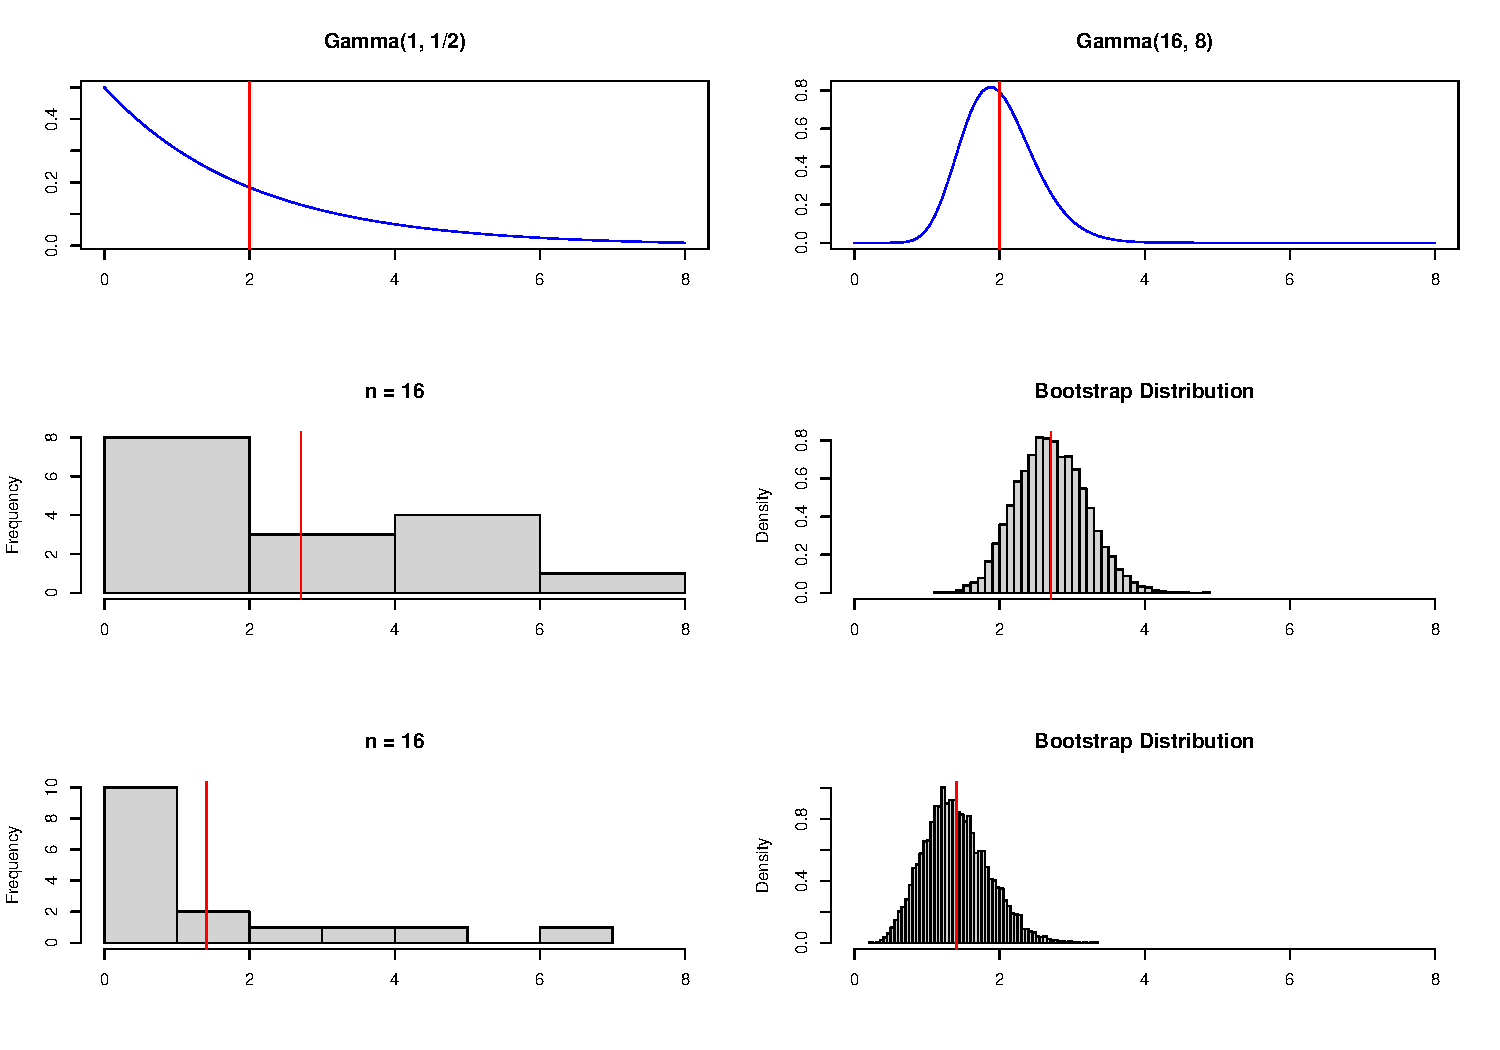
\includegraphics[width=0.9\linewidth,height=0.75\textheight]{Week10_Lect_files/figure-beamer/unnamed-chunk-5-1} \end{center}
\normalsize
\end{frame}

\begin{frame}{Key features of the Bootstrap: Example 2}
\protect\hypertarget{key-features-of-the-bootstrap-example-2-3}{}
\begin{itemize}
\item
  The first graph in the second and third rows shows the distribution of
  a random sample with sample means and standard deviations

  \begin{itemize}
  \tightlist
  \item
    \(\bar{x}_1= 2.7101126\) and, \(\bar{x}_2=1.404806\)
  \item
    \(s_1= 1.98708\) and, \(s_2=1.79941\)
  \end{itemize}
\item
  Based on the graphs above, we can see that the bootstrap distribution:

  \begin{itemize}
  \tightlist
  \item
    has roughly the same spread and shape as the theoretical sampling
    distribution,
  \item
    but the centers are different compared to the theoretical sampling
    distribution.
  \end{itemize}
\end{itemize}
\end{frame}

\begin{frame}{Key features of the Bootstrap}
\protect\hypertarget{key-features-of-the-bootstrap-1}{}
For most common estimators and under fairly general distribution
assumptions, the following need to be noted:

\begin{itemize}
\item
  \textbf{Center}: The center of the bootstrap distribution is not an
  accurate approximation for the center of the sampling distribution.

  \begin{itemize}
  \tightlist
  \item
    For example, the center of the bootstrap distribution for
    \(\bar{X}\) is centered at approximately \(\bar{x}=\mu_{\hat{F}}\),
    the mean of the sample, whereas
  \item
    the sampling distribution is centered at \(\mu\).
  \end{itemize}
\item
  \textbf{Spread}: The spread of the bootstrap distribution does reflect
  the spread of the sampling distribution.
\item
  \textbf{Bias}: The bootstrap bias estimate does reflect the bias of
  the sampling distribution. Bias occurs if a sampling distribution is
  not centered at the parameter.
\item
  \textbf{Skewness}: The skewness of the bootstrap distribution does
  reflect the skewness of the sampling distribution.
\end{itemize}
\end{frame}

\begin{frame}{Key features of the Bootstrap}
\protect\hypertarget{key-features-of-the-bootstrap-2}{}
\begin{itemize}
\item
  The first point bears emphasis.

  \begin{itemize}
  \tightlist
  \item
    It means that the bootstrap is not used to get better parameter
    estimates because the bootstrap distributions are centered around
    statistics \(\hat{\theta}\) calculated from the data rather than
    unknown population values.
  \item
    Drawing thousands of bootstrap observations from the original data
    is not like drawing observations from the underlying population, it
    does not create new data.
  \end{itemize}
\item
  Instead, the bootstrap distribution is useful for quantifying the
  behavior of a parameter estimate such as its :

  \begin{itemize}
  \tightlist
  \item
    standard error,
  \item
    skewness, bias, or
  \item
    for calculating confidence intervals.
  \end{itemize}
\end{itemize}
\end{frame}

\begin{frame}{Key features of the Bootstrap: Example 3}
\protect\hypertarget{key-features-of-the-bootstrap-example-3}{}
\begin{tcolorbox}
Arsenic is a naturally occurring element in the groundwater of Bangladesh. However, much of this groundwater is used for drinking water by rural populations, so arsenic poisoning is a serious health issue. Figure 1a displays the distribution of arsenic concentrations from 271 wells in Bangladesh. The sample mean and standard deviation are $\bar{x}=125.32$ and $s =297.98$, respectively (measured in micrograms per liter). We draw resamples of size 271 with replacement from the data and compute the mean for each resample.
\end{tcolorbox}
\end{frame}

\begin{frame}[fragile]{Key features of the Bootstrap: Example 3}
\protect\hypertarget{key-features-of-the-bootstrap-example-3-1}{}
\tiny

\begin{Shaded}
\begin{Highlighting}[]
\FunctionTok{par}\NormalTok{(}\AttributeTok{mfrow =} \FunctionTok{c}\NormalTok{(}\DecValTok{2}\NormalTok{, }\DecValTok{2}\NormalTok{))}
\NormalTok{Bang }\OtherTok{\textless{}{-}}\NormalTok{ Bangladesh}
\NormalTok{Arsenic }\OtherTok{\textless{}{-}}\NormalTok{ Bang}\SpecialCharTok{$}\NormalTok{Arsenic}
\FunctionTok{hist}\NormalTok{(Arsenic, }\AttributeTok{breaks =} \StringTok{"Scott"}\NormalTok{, }\AttributeTok{main =} \StringTok{"Figure 1a"}\NormalTok{, }\AttributeTok{col =} \StringTok{"lightblue"}\NormalTok{)}
\FunctionTok{qqnorm}\NormalTok{(Arsenic, }\AttributeTok{main =} \StringTok{"Figure 1b"}\NormalTok{)}
\FunctionTok{qqline}\NormalTok{(Arsenic, }\AttributeTok{col =} \StringTok{"red"}\NormalTok{)}
\NormalTok{B }\OtherTok{\textless{}{-}} \DecValTok{10000}
\NormalTok{n }\OtherTok{\textless{}{-}} \FunctionTok{sum}\NormalTok{(}\SpecialCharTok{!}\FunctionTok{is.na}\NormalTok{(Arsenic))}
\NormalTok{arsenic.mean }\OtherTok{\textless{}{-}} \FunctionTok{numeric}\NormalTok{(B)}
\FunctionTok{set.seed}\NormalTok{(}\DecValTok{7}\NormalTok{)}
\ControlFlowTok{for}\NormalTok{ (i }\ControlFlowTok{in} \DecValTok{1}\SpecialCharTok{:}\NormalTok{B)\{}
\NormalTok{  bss }\OtherTok{\textless{}{-}} \FunctionTok{sample}\NormalTok{(Arsenic, }\AttributeTok{size =}\NormalTok{ n, }\AttributeTok{replace =} \ConstantTok{TRUE}\NormalTok{)}
\NormalTok{  arsenic.mean[i] }\OtherTok{\textless{}{-}} \FunctionTok{mean}\NormalTok{(bss)}
\NormalTok{\}}
\FunctionTok{hist}\NormalTok{(arsenic.mean, }\AttributeTok{main =} \StringTok{"Figure 2a"}\NormalTok{, }\AttributeTok{col =} \StringTok{"lightblue"}\NormalTok{, }\AttributeTok{breaks =} \StringTok{"Scott"}\NormalTok{, }
     \AttributeTok{xlab =} \FunctionTok{substitute}\NormalTok{(}\FunctionTok{paste}\NormalTok{(}\FunctionTok{bar}\NormalTok{(X),}\StringTok{"*"}\NormalTok{)))}
\FunctionTok{qqnorm}\NormalTok{(arsenic.mean, }\AttributeTok{main =} \StringTok{"Figure 2b"}\NormalTok{)}
\FunctionTok{qqline}\NormalTok{(arsenic.mean, }\AttributeTok{col =} \StringTok{"red"}\NormalTok{)}
\end{Highlighting}
\end{Shaded}

\normalsize
\end{frame}

\begin{frame}{Key features of the Bootstrap: Example 3}
\protect\hypertarget{key-features-of-the-bootstrap-example-3-2}{}
\tiny

\begin{center}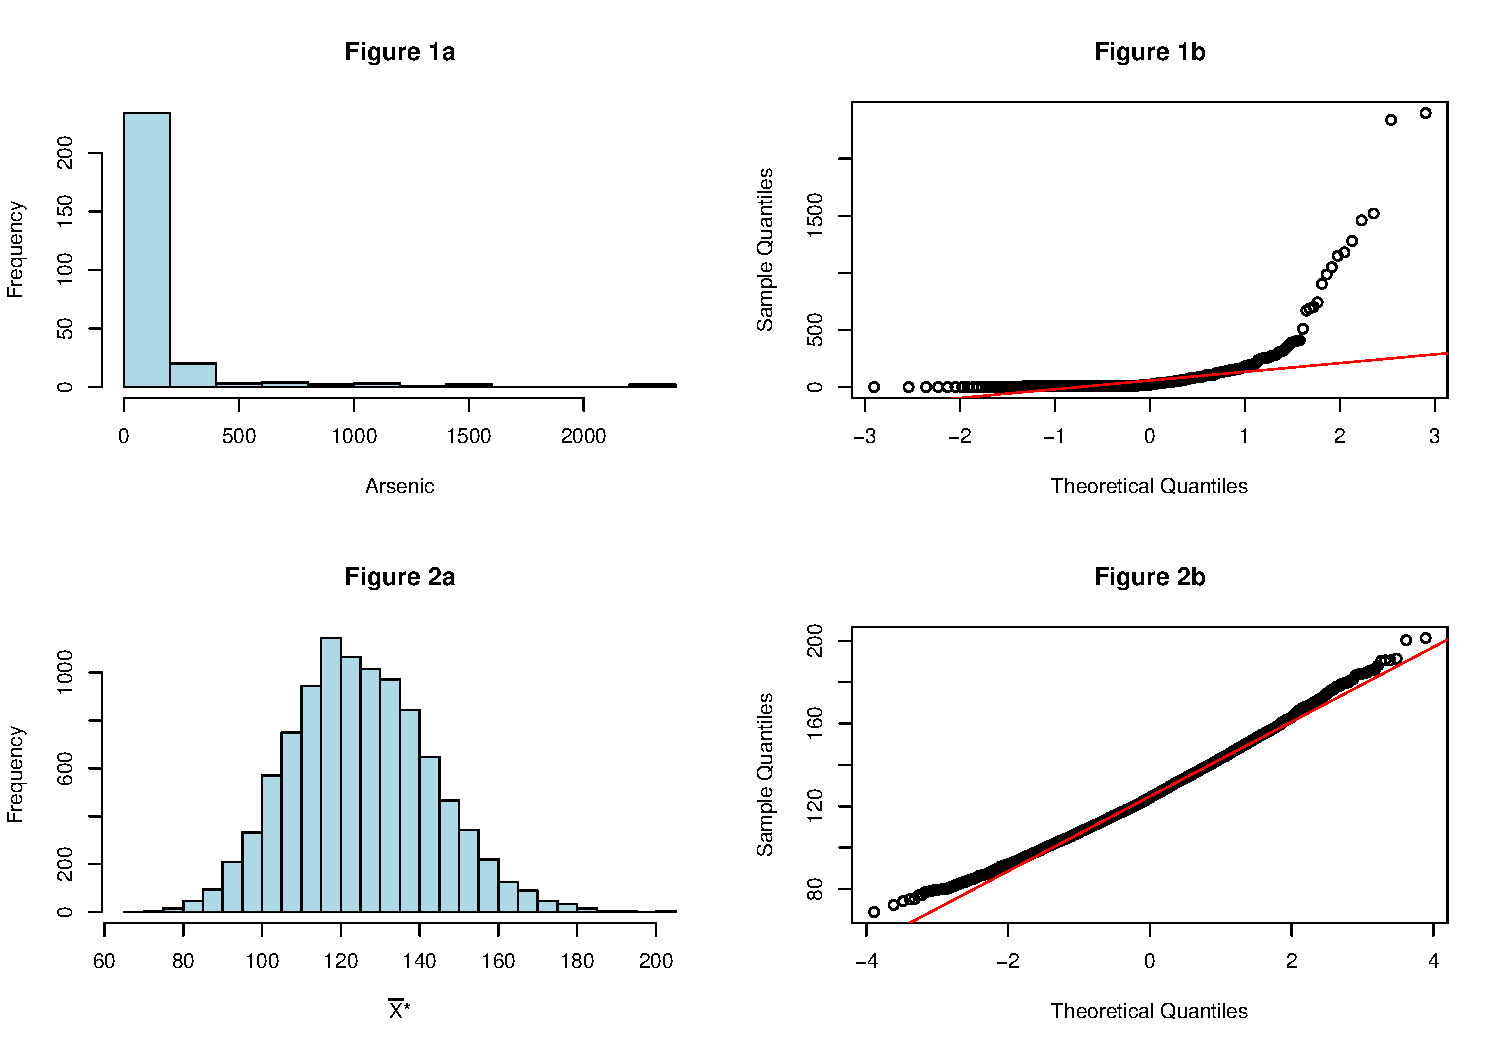
\includegraphics[width=0.9\linewidth,height=0.85\textheight]{Week10_Lect_files/figure-beamer/unnamed-chunk-7-1} \end{center}
\normalsize
\end{frame}

\begin{frame}{Key features of the Bootstrap: Example 3}
\protect\hypertarget{key-features-of-the-bootstrap-example-3-3}{}
\begin{itemize}
\item
  Figures 2a and 2b show a histogram and a normal quantile plot of the
  bootstrap distribution, respectively.
\item
  The bootstrap distribution looks quite normal, with some skewness.
\item
  This is the central limit theorem at work---when the sample size is
  large enough, the sampling distribution for the mean is approximately
  normal, even if the population is not normal.
\end{itemize}
\end{frame}

\hypertarget{understanding-confidence-intervals}{%
\section{Understanding confidence
intervals}\label{understanding-confidence-intervals}}

\begin{frame}[fragile]{Understanding confidence intervals}
\protect\hypertarget{understanding-confidence-intervals-1}{}
\begin{itemize}
\item
  Let's start this section with an analogy involving fishing. Say you
  are trying to catch a fish.

  \begin{itemize}
  \tightlist
  \item
    On one hand, you could use a spear, while on the other
  \item
    you could use a net. Using the net will probably allow you to catch
    more fish!
  \end{itemize}
\item
  Now think back to our pennies exercise where you are trying to
  estimate the true population mean year \(\mu\) of all US pennies.

  \begin{itemize}
  \tightlist
  \item
    Think of the value of \(\mu\) as a fish.
  \end{itemize}
\end{itemize}

\begin{Shaded}
\begin{Highlighting}[]
\NormalTok{pennies\_sample }\SpecialCharTok{\%\textgreater{}\%} 
  \FunctionTok{summarize}\NormalTok{(}\AttributeTok{xbar\_year =} \FunctionTok{mean}\NormalTok{(year))}
\end{Highlighting}
\end{Shaded}

\begin{verbatim}
# A tibble: 1 x 1
  xbar_year
      <dbl>
1     1995.
\end{verbatim}
\end{frame}

\begin{frame}[fragile]{Understanding confidence intervals}
\protect\hypertarget{understanding-confidence-intervals-2}{}
\begin{itemize}
\item
  On the one hand, we could use the appropriate point estimate/sample
  statistic to estimate \(\mu\), with the sample mean \(\bar{x}\).
\item
  Based on our sample of 50 pennies from the bank (using the tibble
  \texttt{pennies\_sample}), the sample mean of \texttt{year} was
  1995.44.
\item
  Think of using this value as ``fishing with a spear.''
\item
  What would ``fishing with a net'' correspond to?

  \begin{itemize}
  \tightlist
  \item
    The bootstrap distribution.
  \item
    Between which two years would you say that ``most'' sample means
    lie?
  \item
    While this question is somewhat subjective, saying that most sample
    means lie between 1992 and 2000 would not be unreasonable.
  \item
    Think of this interval as the ``net.''
  \end{itemize}
\item
  What we've just illustrated is the concept of a confidence interval,
  which we'll abbreviate with ``CI''.
\end{itemize}
\end{frame}

\begin{frame}{Understanding confidence intervals}
\protect\hypertarget{understanding-confidence-intervals-3}{}
\begin{itemize}
\item
  As opposed to a point estimate/sample statistic that estimates the
  value of an unknown population parameter with a single value, a
  \textbf{confidence interval} gives what can be interpreted as a range
  of plausible values.
\item
  Going back to our analogy, point estimates/sample statistics can be
  thought of as spears, whereas confidence intervals can be thought of
  as nets.
\end{itemize}

\begin{center}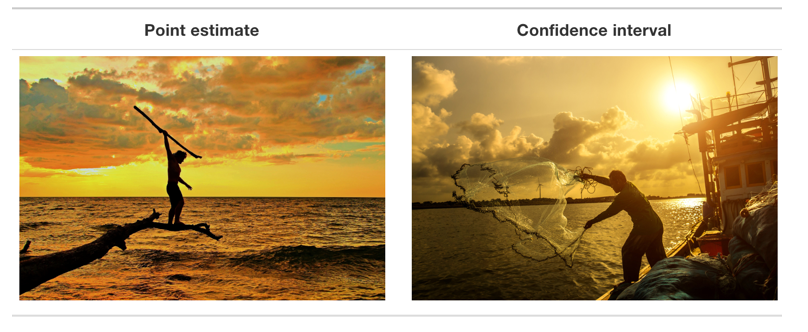
\includegraphics[width=0.7\linewidth,height=0.4\textheight]{week10_7} \end{center}
\end{frame}

\begin{frame}[fragile]{Percentile method}
\protect\hypertarget{percentile-method}{}
\small

\begin{Shaded}
\begin{Highlighting}[]
\NormalTok{pennies\_sample }\SpecialCharTok{\%\textgreater{}\%} 
  \FunctionTok{specify}\NormalTok{(}\AttributeTok{response =}\NormalTok{ year) }\SpecialCharTok{\%\textgreater{}\%} 
  \FunctionTok{generate}\NormalTok{(}\AttributeTok{reps =} \DecValTok{1000}\NormalTok{, }\AttributeTok{type =} \StringTok{"bootstrap"}\NormalTok{) }\SpecialCharTok{\%\textgreater{}\%} 
  \FunctionTok{calculate}\NormalTok{(}\AttributeTok{stat =} \StringTok{"mean"}\NormalTok{) }\OtherTok{{-}\textgreater{}}\NormalTok{ bs\_dist}
\NormalTok{bs\_dist }\SpecialCharTok{\%\textgreater{}\%} 
  \FunctionTok{summarize}\NormalTok{(}\AttributeTok{lci =} \FunctionTok{quantile}\NormalTok{(stat, }\AttributeTok{probs =} \FloatTok{0.025}\NormalTok{), }
            \AttributeTok{uci =} \FunctionTok{quantile}\NormalTok{(stat, }\AttributeTok{probs =} \FloatTok{0.975}\NormalTok{)) }\OtherTok{{-}\textgreater{}}\NormalTok{ CI}
\NormalTok{CI}
\end{Highlighting}
\end{Shaded}

\begin{verbatim}
# A tibble: 1 x 2
    lci   uci
  <dbl> <dbl>
1 1991. 2000.
\end{verbatim}

\normalsize
\end{frame}

\begin{frame}[fragile]{Percentile method}
\protect\hypertarget{percentile-method-1}{}
\small

\begin{Shaded}
\begin{Highlighting}[]
\FunctionTok{get\_confidence\_interval}\NormalTok{(bs\_dist, }\AttributeTok{level =} \FloatTok{0.95}\NormalTok{)}
\end{Highlighting}
\end{Shaded}

\begin{verbatim}
# A tibble: 1 x 2
  lower_ci upper_ci
     <dbl>    <dbl>
1    1991.    2000.
\end{verbatim}

\begin{Shaded}
\begin{Highlighting}[]
\FunctionTok{visualize}\NormalTok{(bs\_dist) }\SpecialCharTok{+} 
  \FunctionTok{shade\_confidence\_interval}\NormalTok{(}\AttributeTok{endpoints =}\NormalTok{ CI)}
\end{Highlighting}
\end{Shaded}

\begin{figure}

{\centering 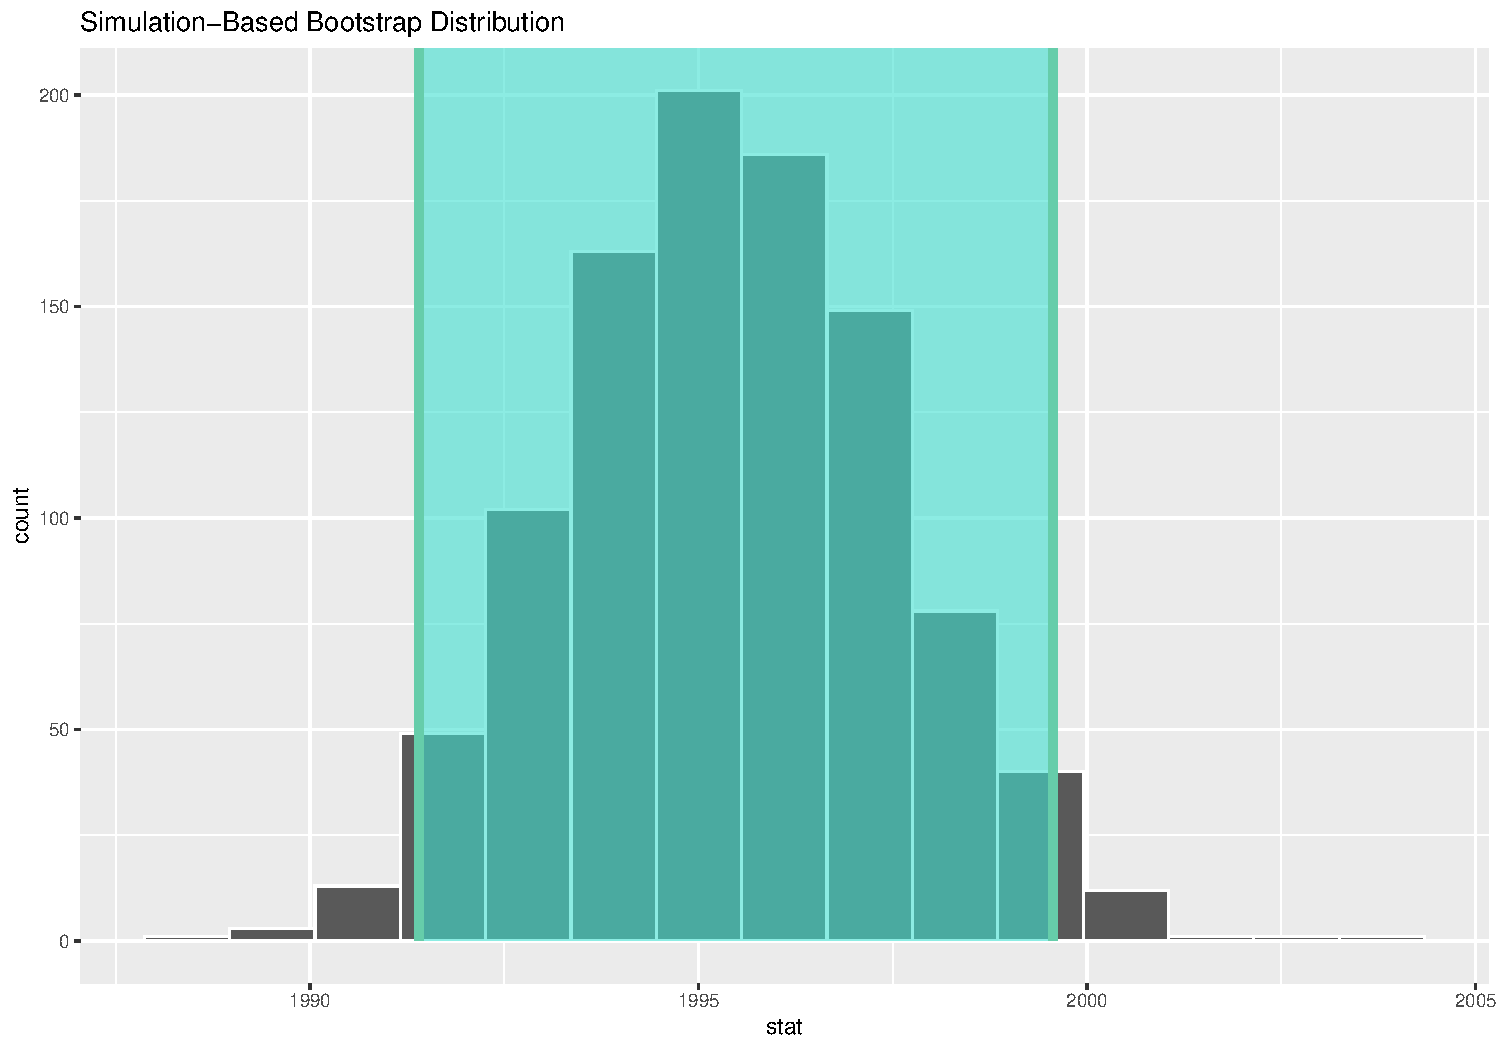
\includegraphics[width=0.5\linewidth,height=0.4\textheight]{Week10_Lect_files/figure-beamer/bsci-1} 

}

\caption{Bootstrap Distribution with percentile CI limits}\label{fig:bsci}
\end{figure}
\normalsize
\end{frame}

\begin{frame}[fragile]{Percentile method}
\protect\hypertarget{percentile-method-2}{}
One method to construct a confidence interval

\begin{itemize}
\item
  To get the middle \(95\%\) of values of the bootstrap distribution:

  \begin{itemize}
  \tightlist
  \item
    We can do this by computing the 2.5th and 97.5th percentiles,
  \item
    which are 1991 and 2000, respectively.
  \item
    This is known as the percentile method for constructing confidence
    intervals.
  \end{itemize}
\end{itemize}

\small

\begin{Shaded}
\begin{Highlighting}[]
\CommentTok{\# Using a for loop to do the same thing}
\NormalTok{B }\OtherTok{\textless{}{-}} \DecValTok{1000}
\NormalTok{bm }\OtherTok{\textless{}{-}} \FunctionTok{numeric}\NormalTok{(B)}
\ControlFlowTok{for}\NormalTok{(i }\ControlFlowTok{in} \DecValTok{1}\SpecialCharTok{:}\NormalTok{B)\{}
\NormalTok{  bss }\OtherTok{\textless{}{-}} \FunctionTok{sample}\NormalTok{(pennies\_sample}\SpecialCharTok{$}\NormalTok{year, }\AttributeTok{size =} \DecValTok{50}\NormalTok{, }\AttributeTok{replace =} \ConstantTok{TRUE}\NormalTok{)}
\NormalTok{  bm[i] }\OtherTok{\textless{}{-}} \FunctionTok{mean}\NormalTok{(bss)}
\NormalTok{\}}
\FunctionTok{quantile}\NormalTok{(bm, }\AttributeTok{probs =} \FunctionTok{c}\NormalTok{(}\FloatTok{0.025}\NormalTok{, }\FloatTok{0.975}\NormalTok{))}
\end{Highlighting}
\end{Shaded}

\begin{verbatim}
    2.5%    97.5% 
1991.519 1999.681 
\end{verbatim}

\normalsize
\end{frame}

\begin{frame}[fragile]{Standard error method}
\protect\hypertarget{standard-error-method}{}
\begin{itemize}
\item
  Given that our bootstrap distribution based on 1000 resamples with
  replacement in Figure 1 is normally shaped,

  \begin{itemize}
  \item
    let's use this fact about normal distributions to construct a
    confidence interval in a different way.
  \item
    First, note that the bootstrap distribution has a mean equal to
    1995.43 (using \texttt{infer} or 1995.52 the for loop).
  \item
    This value almost coincides exactly with the value of the sample
    mean \(\bar{x}\) of our original 50 pennies of 1995.44.
  \end{itemize}
\item
  Second, let's compute the standard deviation of the bootstrap
  distribution using the values of \texttt{mean\_year} in the
  \texttt{virtual\_resampled\_means} data frame:
\end{itemize}
\end{frame}

\begin{frame}[fragile]{Standard error method}
\protect\hypertarget{standard-error-method-1}{}
\small

\begin{Shaded}
\begin{Highlighting}[]
\FunctionTok{set.seed}\NormalTok{(}\DecValTok{10}\NormalTok{)}
\NormalTok{virtual\_resampled\_means }\OtherTok{\textless{}{-}}\NormalTok{ pennies\_sample }\SpecialCharTok{\%\textgreater{}\%} 
  \FunctionTok{rep\_sample\_n}\NormalTok{(}\AttributeTok{size =} \DecValTok{50}\NormalTok{, }\AttributeTok{replace =} \ConstantTok{TRUE}\NormalTok{, }\AttributeTok{reps =} \DecValTok{1000}\NormalTok{) }\SpecialCharTok{\%\textgreater{}\%} 
  \FunctionTok{group\_by}\NormalTok{(replicate) }\SpecialCharTok{\%\textgreater{}\%} 
  \FunctionTok{summarize}\NormalTok{(}\AttributeTok{mean\_year =} \FunctionTok{mean}\NormalTok{(year))}
\NormalTok{virtual\_resampled\_means }\SpecialCharTok{\%\textgreater{}\%} 
  \FunctionTok{summarize}\NormalTok{(}\AttributeTok{SE =} \FunctionTok{sd}\NormalTok{(mean\_year)) }\OtherTok{{-}\textgreater{}}\NormalTok{ ans}
\NormalTok{ans}
\end{Highlighting}
\end{Shaded}

\begin{verbatim}
# A tibble: 1 x 1
     SE
  <dbl>
1  2.14
\end{verbatim}

\begin{Shaded}
\begin{Highlighting}[]
\CommentTok{\# Or}
\FunctionTok{sd}\NormalTok{(bm)}
\end{Highlighting}
\end{Shaded}

\begin{verbatim}
[1] 2.14079
\end{verbatim}
\end{frame}

\begin{frame}[fragile]{Standard error method}
\protect\hypertarget{standard-error-method-2}{}
Recall that for a normal distribution, roughly \(95\%\) of values fall
between \(\pm1.96\) standard deviations of the mean.

\begin{itemize}
\tightlist
\item
  Thus, using our \(95\%\) rule of thumb about normal distributions, we
  can use the following formula to determine the lower and upper
  endpoints of a 95\% confidence interval for \(\mu\).
\end{itemize}

\[\begin{array}{ll}
\bar{x}\pm1.96\cdot SE&=(\bar{x}-1.96\cdot SE, \bar{x}+1.96\cdot SE)\\
&=(1995.44-1.96\cdot 2.14, 1995.44+1.96\cdot2.14)\\
&=(1991.25,1999.63)
\end{array}\]

\begin{Shaded}
\begin{Highlighting}[]
\FunctionTok{mean}\NormalTok{(pennies\_sample}\SpecialCharTok{$}\NormalTok{year) }\SpecialCharTok{+}\FunctionTok{c}\NormalTok{(}\SpecialCharTok{{-}}\DecValTok{1}\NormalTok{, }\DecValTok{1}\NormalTok{)}\SpecialCharTok{*}\FunctionTok{qnorm}\NormalTok{(.}\DecValTok{975}\NormalTok{)}\SpecialCharTok{*}\NormalTok{ans}\SpecialCharTok{$}\NormalTok{SE}
\end{Highlighting}
\end{Shaded}

\begin{verbatim}
[1] 1991.251 1999.629
\end{verbatim}
\end{frame}

\begin{frame}{Standard error method vs.~Percentile method}
\protect\hypertarget{standard-error-method-vs.-percentile-method}{}
\begin{itemize}
\item
  We see that both methods produce nearly identical \(95\%\) confidence
  intervals for \(\mu\)

  \begin{itemize}
  \tightlist
  \item
    with the percentile method yielding \((1991, 2000)\)
  \item
    while the standard error method produces \((1991.25, 1999.63)\)
  \end{itemize}
\item
  However, we can only use the standard error rule when the bootstrap
  distribution is roughly normally shaped.
\end{itemize}
\end{frame}

\hypertarget{constructing-confidence-intervals}{%
\section{Constructing confidence
intervals}\label{constructing-confidence-intervals}}

\begin{frame}[fragile]{Percentile method example: Pennies Activity}
\protect\hypertarget{percentile-method-example-pennies-activity}{}
Using \texttt{rep\_sample\_n} from the \texttt{infer} package.

\tiny

\begin{Shaded}
\begin{Highlighting}[]
\FunctionTok{set.seed}\NormalTok{(}\DecValTok{10}\NormalTok{)}
\NormalTok{virtual\_resampled\_means }\OtherTok{\textless{}{-}}\NormalTok{ pennies\_sample }\SpecialCharTok{\%\textgreater{}\%} 
  \FunctionTok{rep\_sample\_n}\NormalTok{(}\AttributeTok{size =} \DecValTok{50}\NormalTok{, }\AttributeTok{replace =} \ConstantTok{TRUE}\NormalTok{, }\AttributeTok{reps =} \DecValTok{1000}\NormalTok{) }\SpecialCharTok{\%\textgreater{}\%} 
  \FunctionTok{group\_by}\NormalTok{(replicate) }\SpecialCharTok{\%\textgreater{}\%} 
  \FunctionTok{summarize}\NormalTok{(}\AttributeTok{mean\_year =} \FunctionTok{mean}\NormalTok{(year))}
\FunctionTok{ggplot}\NormalTok{(virtual\_resampled\_means, }\FunctionTok{aes}\NormalTok{(}\AttributeTok{x =}\NormalTok{ mean\_year)) }\SpecialCharTok{+}
  \FunctionTok{geom\_histogram}\NormalTok{(}\AttributeTok{binwidth =} \DecValTok{1}\NormalTok{, }\AttributeTok{color =} \StringTok{"white"}\NormalTok{, }\AttributeTok{boundary =} \DecValTok{1990}\NormalTok{) }\SpecialCharTok{+}
  \FunctionTok{labs}\NormalTok{(}\AttributeTok{x =} \StringTok{"sample mean"}\NormalTok{) }\SpecialCharTok{+}
  \FunctionTok{theme\_bw}\NormalTok{()}
\end{Highlighting}
\end{Shaded}

\begin{center}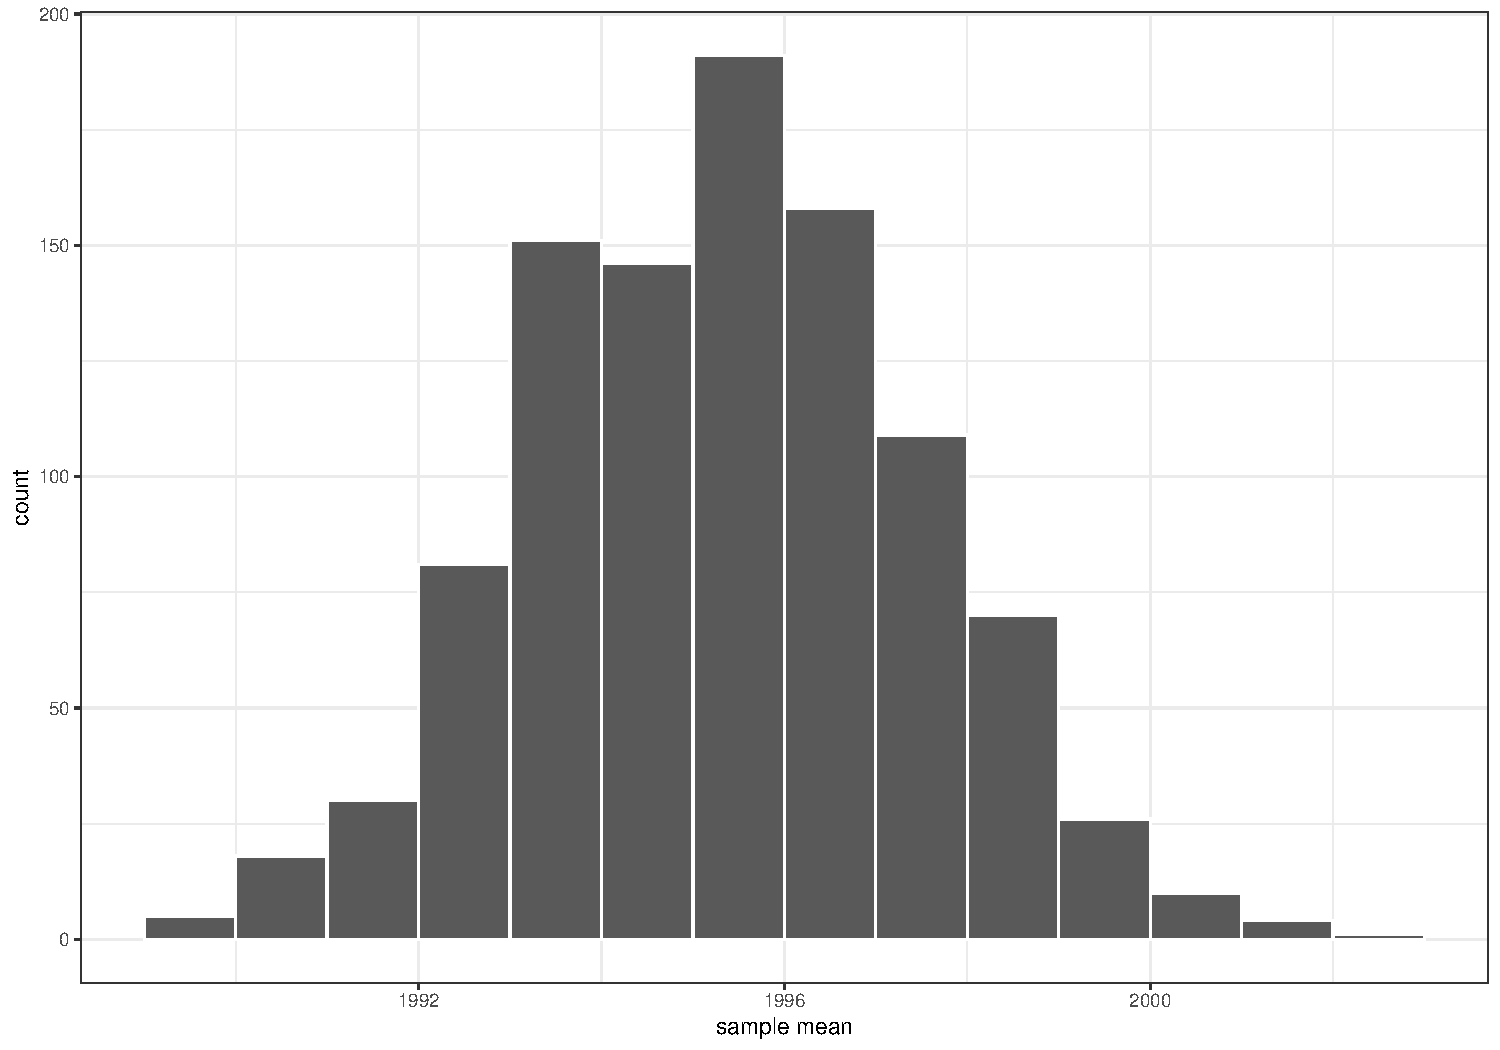
\includegraphics[width=0.6\linewidth,height=0.4\textheight]{Week10_Lect_files/figure-beamer/unnamed-chunk-14-1} \end{center}
\normalsize
\end{frame}

\begin{frame}[fragile]{Percentile method example: Pennies Activity}
\protect\hypertarget{percentile-method-example-pennies-activity-1}{}
Using \texttt{rep\_sample\_n} from the \texttt{infer} package.

\begin{Shaded}
\begin{Highlighting}[]
\FunctionTok{quantile}\NormalTok{(virtual\_resampled\_means}\SpecialCharTok{$}\NormalTok{mean\_year, }
         \AttributeTok{prob =} \FunctionTok{c}\NormalTok{(}\FloatTok{0.025}\NormalTok{, }\FloatTok{0.975}\NormalTok{))}
\end{Highlighting}
\end{Shaded}

\begin{verbatim}
    2.5%    97.5% 
1991.099 1999.460 
\end{verbatim}
\end{frame}

\begin{frame}[fragile]{Percentile method example: Pennies Activity}
\protect\hypertarget{percentile-method-example-pennies-activity-2}{}
Using the \texttt{infer} pipeline

\tiny

\begin{Shaded}
\begin{Highlighting}[]
\FunctionTok{set.seed}\NormalTok{(}\DecValTok{10}\NormalTok{)}
\NormalTok{bootstrap\_distribution }\OtherTok{\textless{}{-}}\NormalTok{ pennies\_sample }\SpecialCharTok{\%\textgreater{}\%} 
  \FunctionTok{specify}\NormalTok{(}\AttributeTok{response =}\NormalTok{ year) }\SpecialCharTok{\%\textgreater{}\%} 
  \FunctionTok{generate}\NormalTok{(}\AttributeTok{reps =} \DecValTok{1000}\NormalTok{, }\AttributeTok{type =} \StringTok{"bootstrap"}\NormalTok{) }\SpecialCharTok{\%\textgreater{}\%} 
  \FunctionTok{calculate}\NormalTok{(}\AttributeTok{stat =} \StringTok{"mean"}\NormalTok{)}
\FunctionTok{visualize}\NormalTok{(bootstrap\_distribution)}
\end{Highlighting}
\end{Shaded}

\begin{center}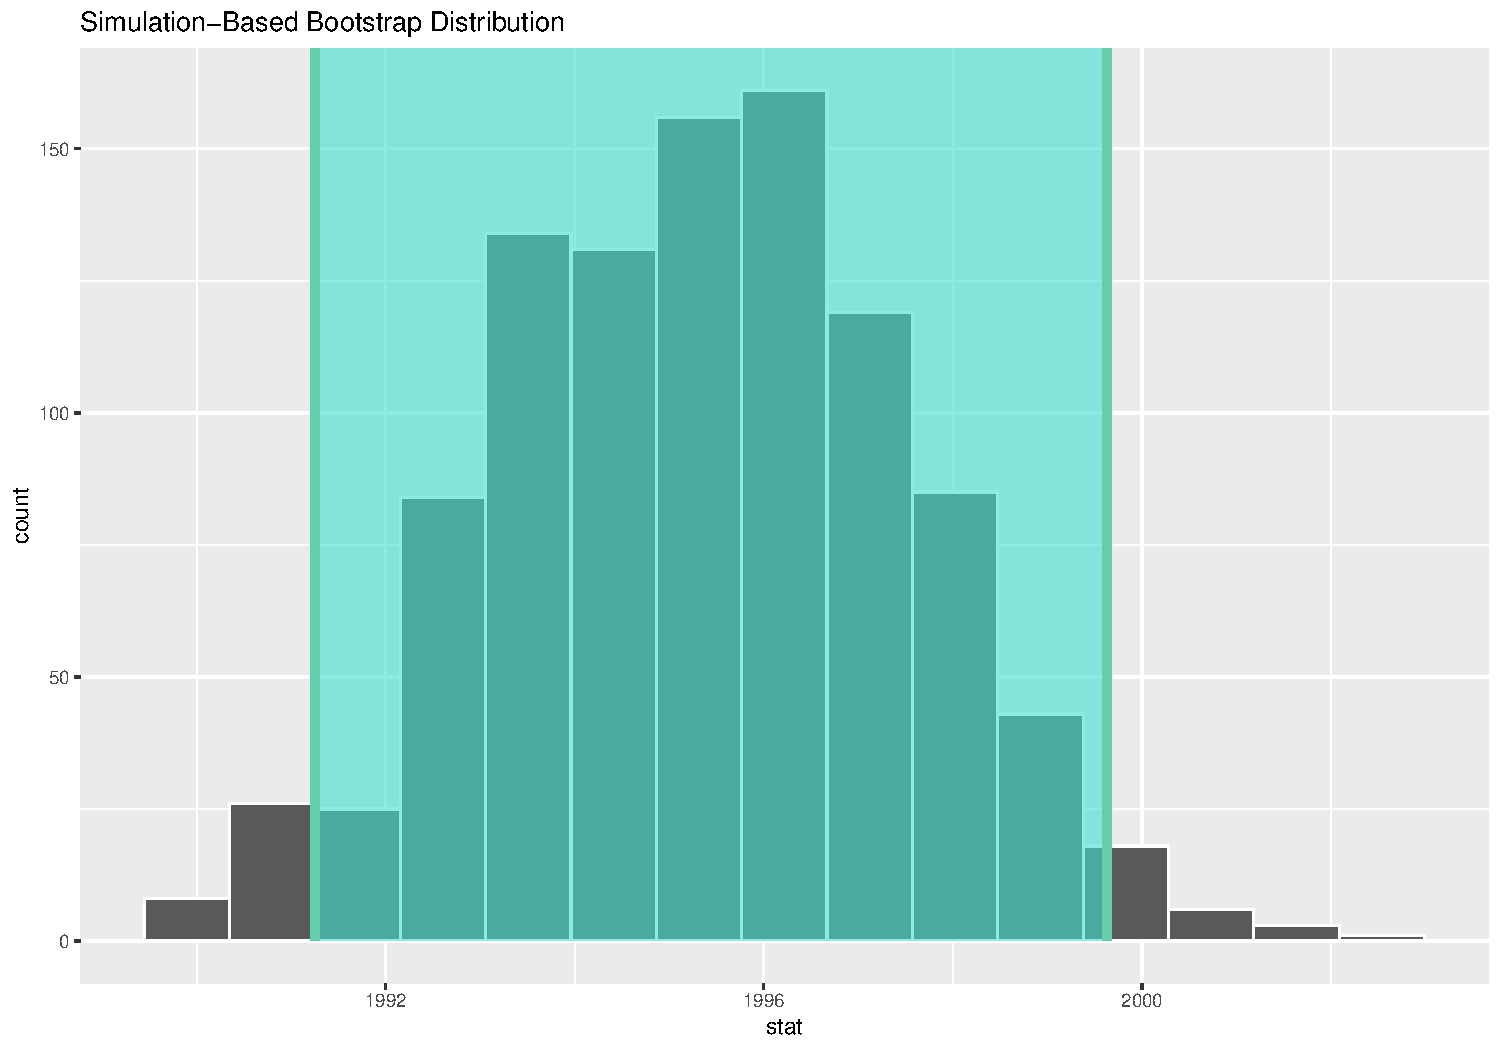
\includegraphics[width=0.7\linewidth,height=0.5\textheight]{Week10_Lect_files/figure-beamer/unnamed-chunk-16-1} \end{center}
\normalsize
\end{frame}

\begin{frame}[fragile]{Percentile method example: Pennies Activity}
\protect\hypertarget{percentile-method-example-pennies-activity-3}{}
Using the \texttt{infer} pipeline

\tiny

\begin{Shaded}
\begin{Highlighting}[]
\NormalTok{percentile\_ci }\OtherTok{\textless{}{-}}\NormalTok{ bootstrap\_distribution }\SpecialCharTok{\%\textgreater{}\%} 
  \FunctionTok{get\_confidence\_interval}\NormalTok{(}\AttributeTok{level =} \FloatTok{0.95}\NormalTok{, }\AttributeTok{type =} \StringTok{"percentile"}\NormalTok{)}
\NormalTok{percentile\_ci}
\end{Highlighting}
\end{Shaded}

\begin{verbatim}
# A tibble: 1 x 2
  lower_ci upper_ci
     <dbl>    <dbl>
1    1991.    1999.
\end{verbatim}

\begin{Shaded}
\begin{Highlighting}[]
\FunctionTok{visualize}\NormalTok{(bootstrap\_distribution) }\SpecialCharTok{+} 
  \FunctionTok{shade\_confidence\_interval}\NormalTok{(}\AttributeTok{endpoints =}\NormalTok{ percentile\_ci)}
\end{Highlighting}
\end{Shaded}

\begin{center}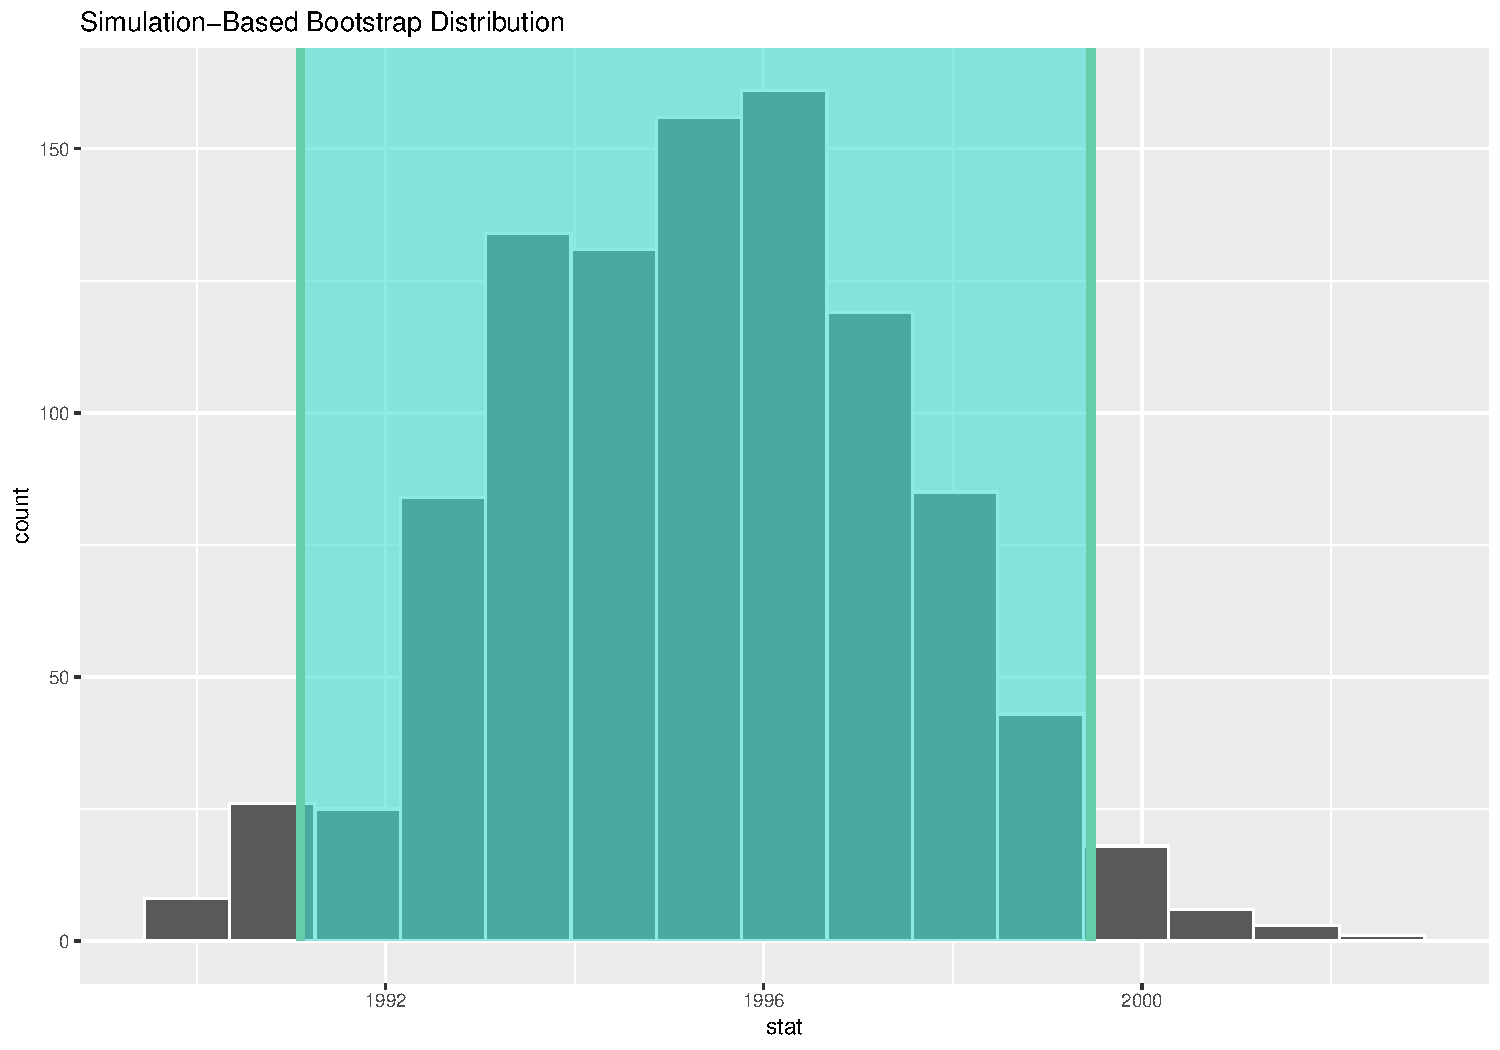
\includegraphics[width=0.7\linewidth,height=0.4\textheight]{Week10_Lect_files/figure-beamer/unnamed-chunk-17-1} \end{center}
\normalsize
\end{frame}

\begin{frame}[fragile]{Standard error example: Pennies Activity}
\protect\hypertarget{standard-error-example-pennies-activity}{}
Using the \texttt{infer} pipeline

\tiny

\begin{Shaded}
\begin{Highlighting}[]
\NormalTok{x\_bar }\OtherTok{\textless{}{-}}\NormalTok{ pennies\_sample }\SpecialCharTok{\%\textgreater{}\%} \FunctionTok{summarize}\NormalTok{(}\AttributeTok{mean\_year =} \FunctionTok{mean}\NormalTok{(year))}
\NormalTok{standard\_error\_ci }\OtherTok{\textless{}{-}}\NormalTok{ bootstrap\_distribution }\SpecialCharTok{\%\textgreater{}\%} 
  \FunctionTok{get\_confidence\_interval}\NormalTok{(}\AttributeTok{type =} \StringTok{"se"}\NormalTok{, }\AttributeTok{point\_estimate =}\NormalTok{ x\_bar, }\AttributeTok{level =} \FloatTok{0.95}\NormalTok{)}
\NormalTok{standard\_error\_ci}
\end{Highlighting}
\end{Shaded}

\begin{verbatim}
# A tibble: 1 x 2
  lower_ci upper_ci
     <dbl>    <dbl>
1    1991.    2000.
\end{verbatim}

\begin{Shaded}
\begin{Highlighting}[]
\FunctionTok{visualize}\NormalTok{(bootstrap\_distribution) }\SpecialCharTok{+} 
  \FunctionTok{shade\_confidence\_interval}\NormalTok{(}\AttributeTok{endpoints =}\NormalTok{ standard\_error\_ci)}
\end{Highlighting}
\end{Shaded}

\begin{center}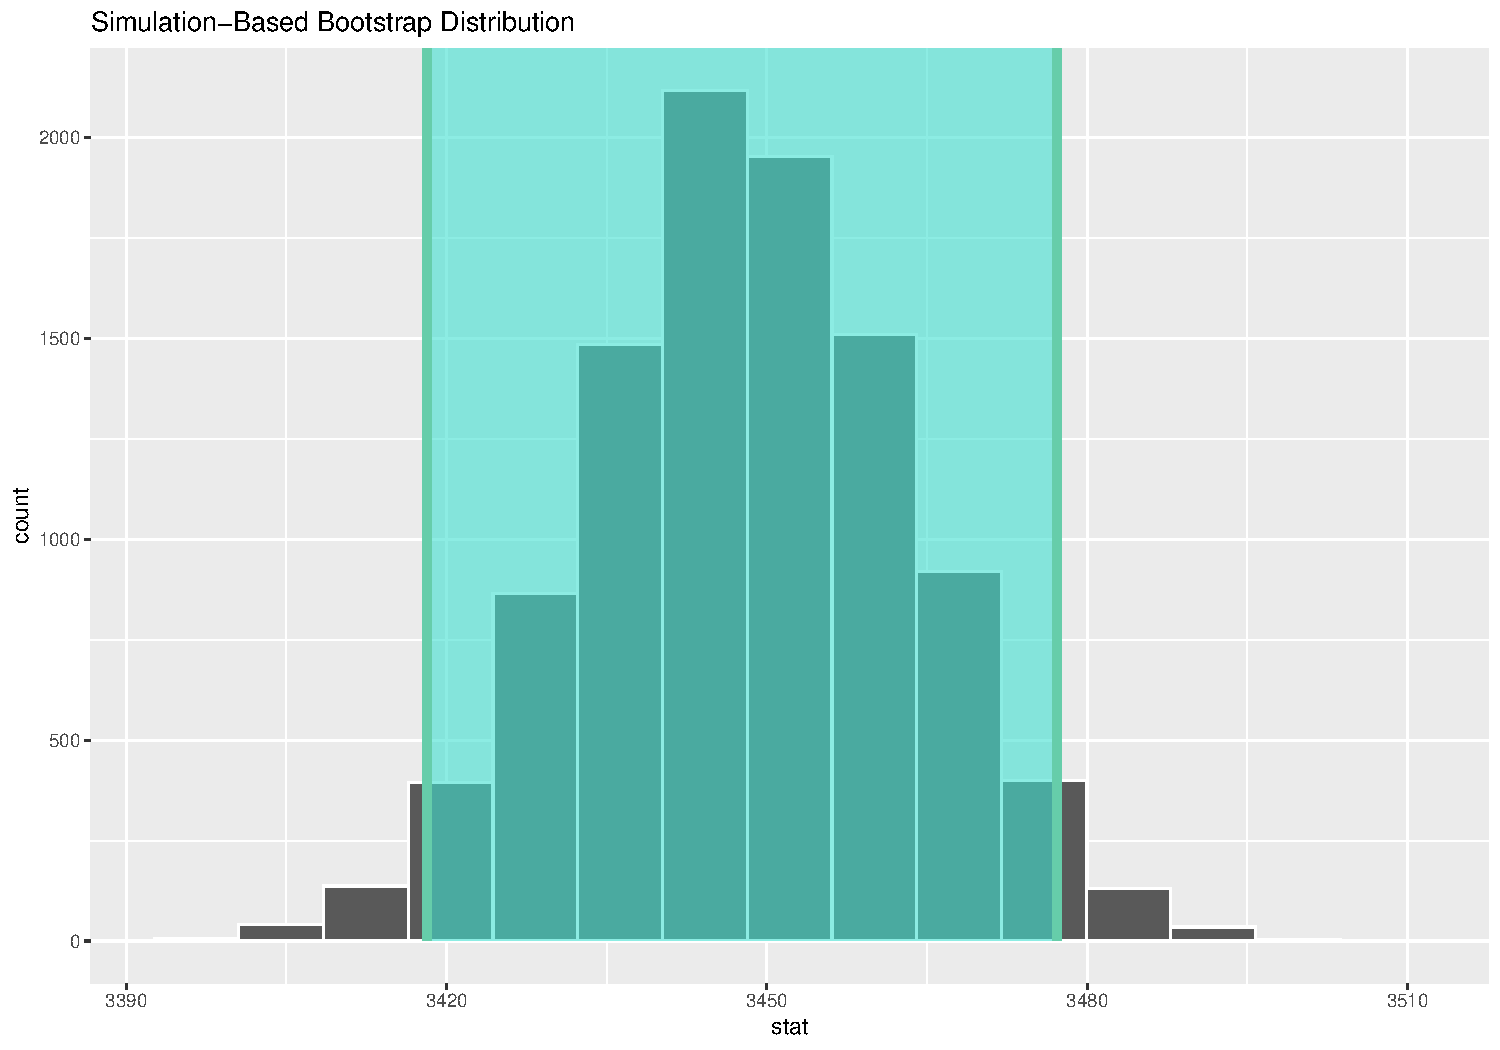
\includegraphics[width=0.7\linewidth,height=0.4\textheight]{Week10_Lect_files/figure-beamer/unnamed-chunk-18-1} \end{center}
\normalsize
\end{frame}

\begin{frame}[fragile]{Percentile method example: Birth weight of a
baby}
\protect\hypertarget{percentile-method-example-birth-weight-of-a-baby}{}
Using the \texttt{infer} pipeline

\tiny

\begin{Shaded}
\begin{Highlighting}[]
\FunctionTok{library}\NormalTok{(resampledata)}
\NormalTok{Babies }\OtherTok{\textless{}{-}}\NormalTok{ NCBirths2004}
\FunctionTok{set.seed}\NormalTok{(}\DecValTok{13}\NormalTok{)}
\NormalTok{bsd }\OtherTok{\textless{}{-}}\NormalTok{ Babies }\SpecialCharTok{\%\textgreater{}\%} 
  \FunctionTok{specify}\NormalTok{(}\AttributeTok{response =}\NormalTok{ Weight) }\SpecialCharTok{\%\textgreater{}\%} 
  \FunctionTok{generate}\NormalTok{(}\AttributeTok{reps =} \DecValTok{10}\SpecialCharTok{\^{}}\DecValTok{4}\NormalTok{, }\AttributeTok{type =} \StringTok{"bootstrap"}\NormalTok{) }\SpecialCharTok{\%\textgreater{}\%} 
  \FunctionTok{calculate}\NormalTok{(}\AttributeTok{stat =} \StringTok{"mean"}\NormalTok{)}
\FunctionTok{visualize}\NormalTok{(bsd)}
\end{Highlighting}
\end{Shaded}

\begin{center}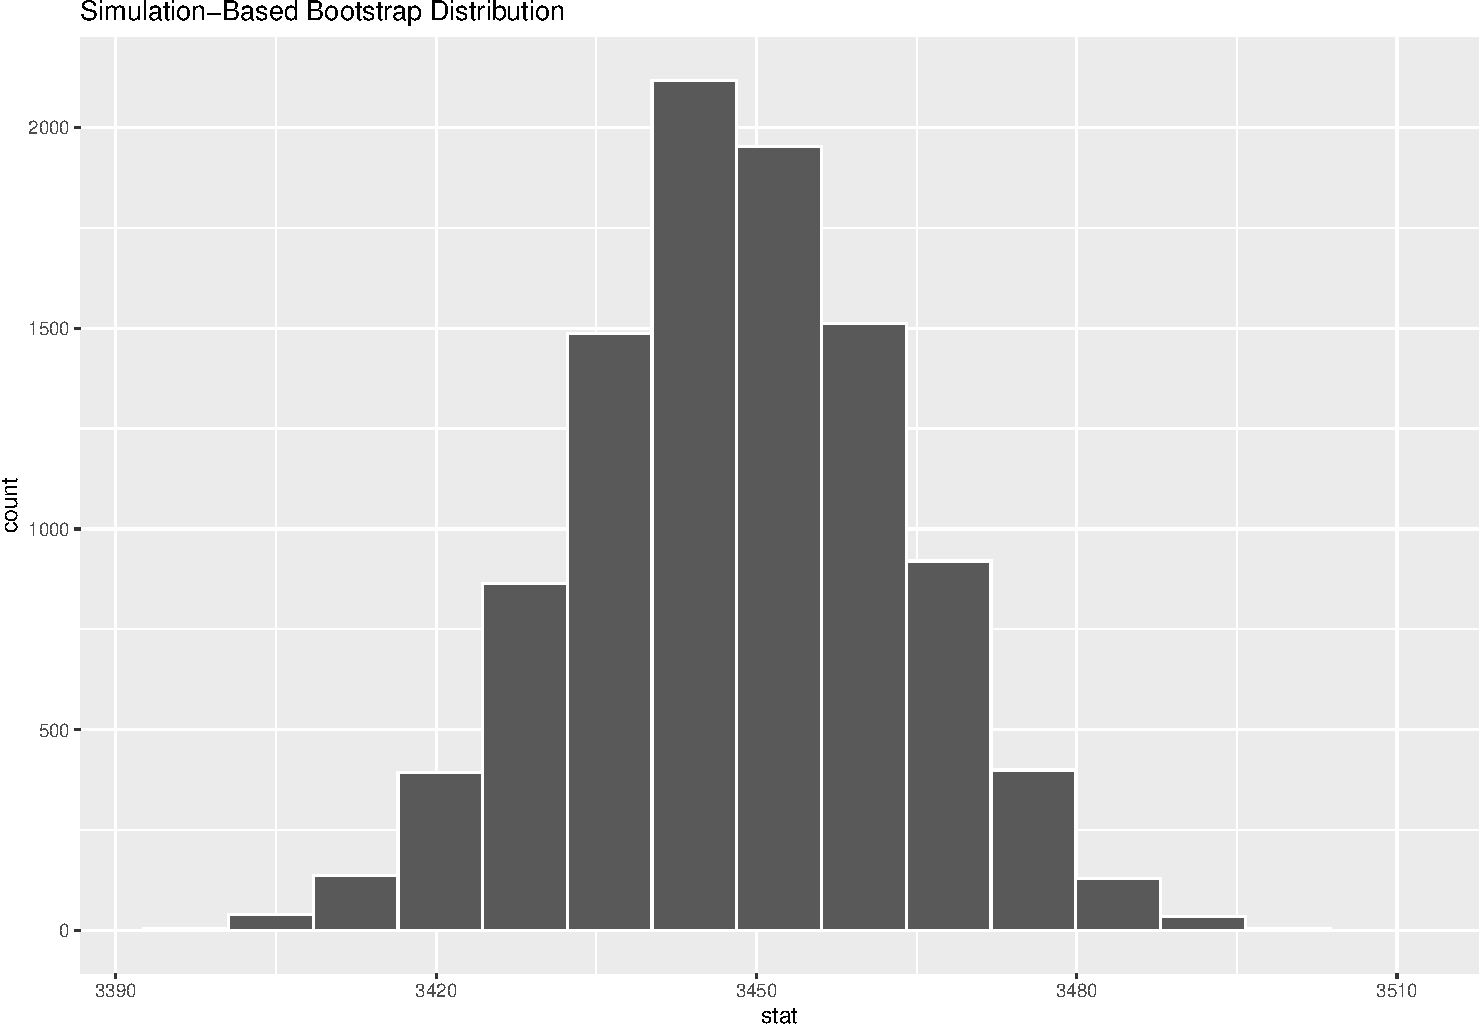
\includegraphics[width=0.7\linewidth,height=0.45\textheight]{Week10_Lect_files/figure-beamer/unnamed-chunk-19-1} \end{center}
\normalsize
\end{frame}

\begin{frame}[fragile]{Percentile method example: Birth weight of a
baby}
\protect\hypertarget{percentile-method-example-birth-weight-of-a-baby-1}{}
Using the \texttt{infer} pipeline

\tiny

\begin{Shaded}
\begin{Highlighting}[]
\NormalTok{percentile\_ci }\OtherTok{\textless{}{-}}\NormalTok{ bsd }\SpecialCharTok{\%\textgreater{}\%} 
  \FunctionTok{get\_confidence\_interval}\NormalTok{(}\AttributeTok{level =} \FloatTok{0.95}\NormalTok{, }\AttributeTok{type =} \StringTok{"percentile"}\NormalTok{)}
\NormalTok{percentile\_ci}
\end{Highlighting}
\end{Shaded}

\begin{verbatim}
# A tibble: 1 x 2
  lower_ci upper_ci
     <dbl>    <dbl>
1    3418.    3477.
\end{verbatim}

\begin{Shaded}
\begin{Highlighting}[]
\FunctionTok{visualize}\NormalTok{(bsd) }\SpecialCharTok{+} 
  \FunctionTok{shade\_confidence\_interval}\NormalTok{(}\AttributeTok{endpoints =}\NormalTok{ percentile\_ci)}
\end{Highlighting}
\end{Shaded}

\begin{center}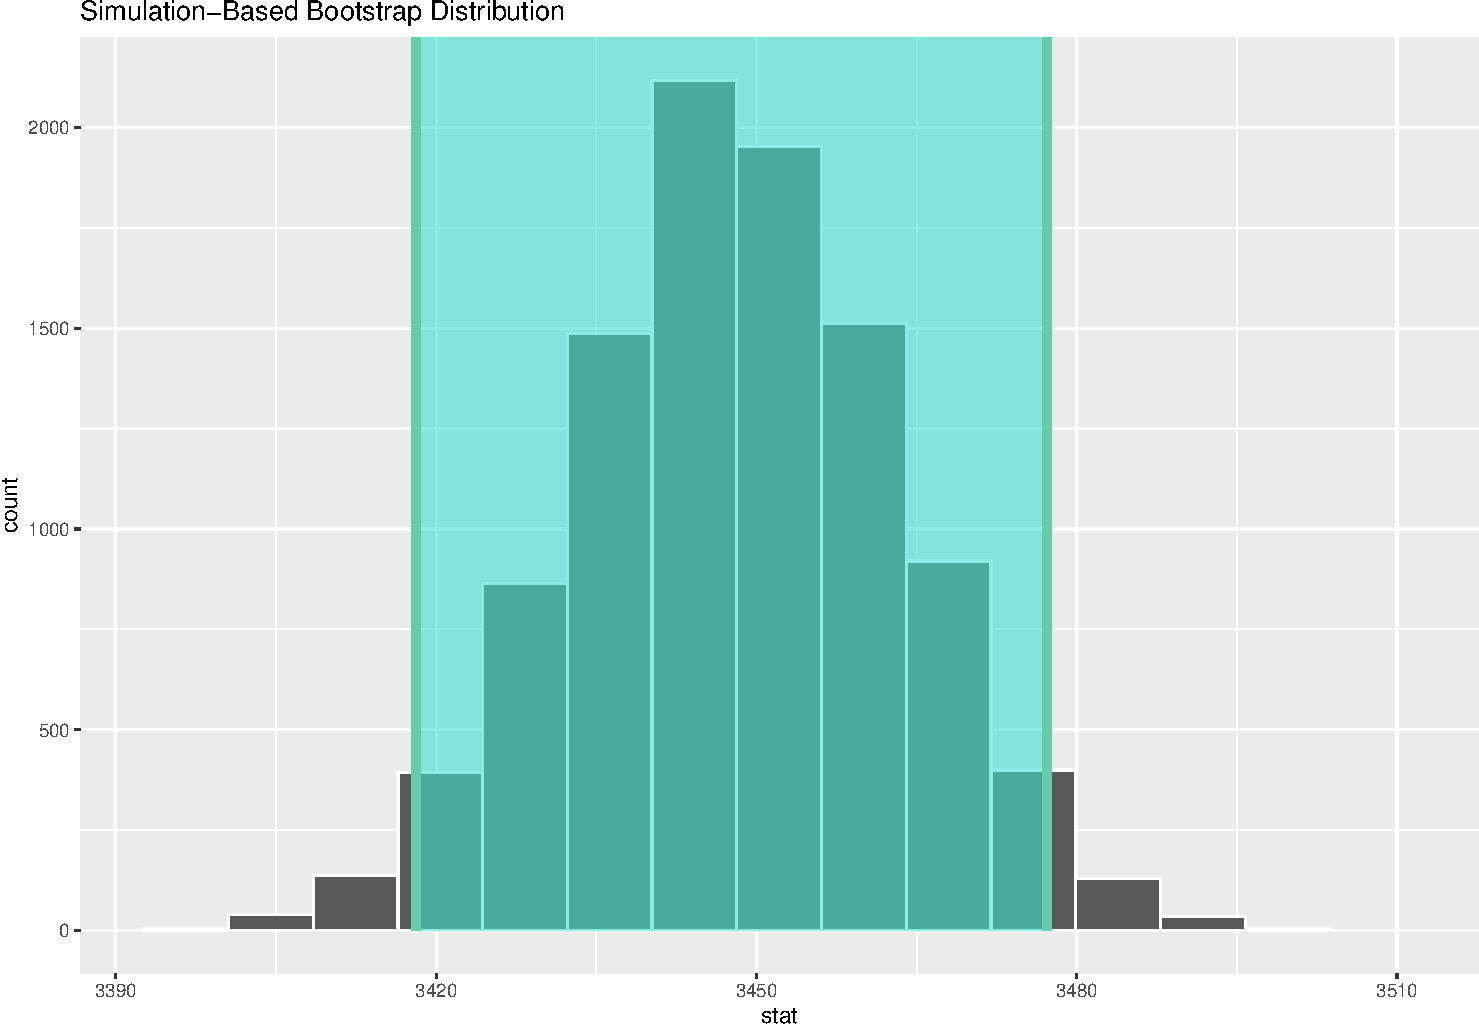
\includegraphics[width=0.7\linewidth,height=0.45\textheight]{Week10_Lect_files/figure-beamer/unnamed-chunk-20-1} \end{center}
\normalsize
\end{frame}

\begin{frame}[fragile]{Standard error example: Birth weight of a baby}
\protect\hypertarget{standard-error-example-birth-weight-of-a-baby}{}
Using the \texttt{infer} pipeline

\tiny

\begin{Shaded}
\begin{Highlighting}[]
\NormalTok{x\_bar\_babies }\OtherTok{\textless{}{-}}\NormalTok{ Babies }\SpecialCharTok{\%\textgreater{}\%} \FunctionTok{summarize}\NormalTok{(}\AttributeTok{Mean =} \FunctionTok{mean}\NormalTok{(Weight))}
\NormalTok{standard\_error\_ci }\OtherTok{\textless{}{-}}\NormalTok{ bsd }\SpecialCharTok{\%\textgreater{}\%} 
  \FunctionTok{get\_confidence\_interval}\NormalTok{(}\AttributeTok{type =} \StringTok{"se"}\NormalTok{, }\AttributeTok{point\_estimate =}\NormalTok{ x\_bar\_babies, }\AttributeTok{level =} \FloatTok{0.95}\NormalTok{)}
\NormalTok{standard\_error\_ci}
\end{Highlighting}
\end{Shaded}

\begin{verbatim}
# A tibble: 1 x 2
  lower_ci upper_ci
     <dbl>    <dbl>
1    3419.    3478.
\end{verbatim}

\begin{Shaded}
\begin{Highlighting}[]
\FunctionTok{visualize}\NormalTok{(bsd) }\SpecialCharTok{+} 
  \FunctionTok{shade\_confidence\_interval}\NormalTok{(}\AttributeTok{endpoints =}\NormalTok{ standard\_error\_ci)}
\end{Highlighting}
\end{Shaded}

\begin{center}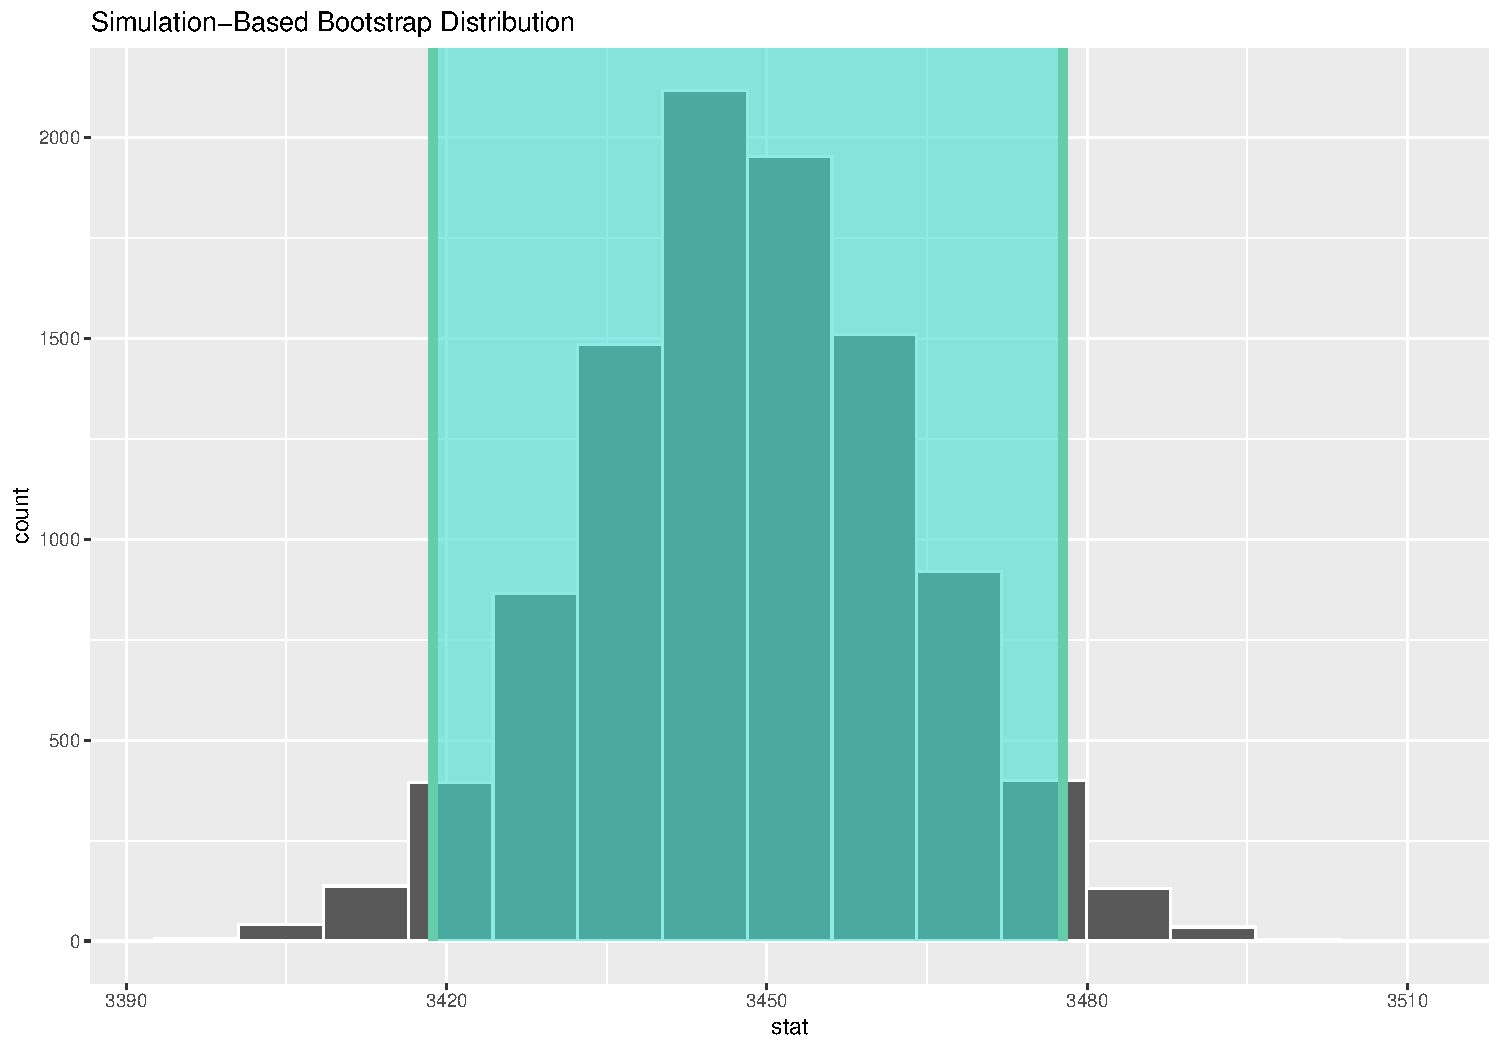
\includegraphics[width=0.7\linewidth,height=0.4\textheight]{Week10_Lect_files/figure-beamer/unnamed-chunk-21-1} \end{center}
\normalsize
\end{frame}

\hypertarget{interpreting-confidence-intervals}{%
\section{Interpreting confidence
intervals}\label{interpreting-confidence-intervals}}

\begin{frame}{Interpreting confidence intervals}
\protect\hypertarget{interpreting-confidence-intervals-1}{}
\begin{itemize}
\item
  Now that we've shown you how to construct confidence intervals using a
  sample drawn from a population, let's now focus on how to interpret
  their effectiveness.
\item
  The effectiveness of a confidence interval is judged by whether or not
  it contains the true value of the population parameter.
\item
  Going back to our fishing analogy, this is like asking, ``Did our net
  capture the fish?''.

  \begin{itemize}
  \tightlist
  \item
    So, for example, does our percentile-based confidence interval of
    (1991.4, 1999.5605) ``capture'' the true mean year \(\mu\) of all US
    pennies?
  \item
    Alas, we'll never know, because we don't know what the true value of
    \(\mu\) is.
  \item
    After all, we're sampling to estimate it!
  \end{itemize}
\end{itemize}
\end{frame}

\begin{frame}[fragile]{Interpreting confidence intervals}
\protect\hypertarget{interpreting-confidence-intervals-2}{}
\begin{itemize}
\item
  In order to interpret a confidence interval's effectiveness, we need
  to know what the value of the population parameter is.

  \begin{itemize}
  \tightlist
  \item
    That way we can say whether or not a confidence interval
    ``captured'' this value.
  \end{itemize}
\item
  Let's revisit our sampling bowl example. What proportion of the bowl's
  2400 balls are red? Let's compute this:
\end{itemize}

\begin{Shaded}
\begin{Highlighting}[]
\NormalTok{bowl }\SpecialCharTok{\%\textgreater{}\%} \FunctionTok{summarize}\NormalTok{(}\AttributeTok{p\_red =} \FunctionTok{mean}\NormalTok{(color }\SpecialCharTok{==} \StringTok{"red"}\NormalTok{))}
\end{Highlighting}
\end{Shaded}

\begin{verbatim}
# A tibble: 1 x 1
  p_red
  <dbl>
1 0.375
\end{verbatim}

In this case we know that the population proportion \(p\) is 0.375. In
other words, we know that \(37.5\%\) of the bowl's balls are red.
\end{frame}

\begin{frame}[fragile]{Interpreting confidence intervals}
\protect\hypertarget{interpreting-confidence-intervals-3}{}
\begin{itemize}
\item
  Recall that we had 33 groups of friends each take samples of size 50
  from the bowl and then compute the sample proportion of red balls
  \(\hat{p}\).

  \begin{itemize}
  \tightlist
  \item
    Let's use the \texttt{bowl\_sample\_1} data frame in the
    \texttt{moderndive} package
  \end{itemize}
\end{itemize}

\small

\begin{Shaded}
\begin{Highlighting}[]
\FunctionTok{head}\NormalTok{(bowl\_sample\_1, }\AttributeTok{n =} \DecValTok{3}\NormalTok{)}
\end{Highlighting}
\end{Shaded}

\begin{verbatim}
# A tibble: 3 x 1
  color
  <chr>
1 white
2 white
3 red  
\end{verbatim}

\begin{Shaded}
\begin{Highlighting}[]
\NormalTok{bowl\_sample\_1 }\SpecialCharTok{\%\textgreater{}\%} 
  \FunctionTok{summarize}\NormalTok{(}\AttributeTok{p\_hat =} \FunctionTok{mean}\NormalTok{(color }\SpecialCharTok{==} \StringTok{"red"}\NormalTok{))}
\end{Highlighting}
\end{Shaded}

\begin{verbatim}
# A tibble: 1 x 1
  p_hat
  <dbl>
1  0.42
\end{verbatim}

\normalsize

\begin{itemize}
\item
  They observed 21 red balls out of 50 and thus their sample proportion
  \(\hat{p}=21/50 = 0.42 = 42\%\).

  \begin{itemize}
  \tightlist
  \item
    Think of this as the ``spear'' from our fishing analogy.
  \end{itemize}
\end{itemize}
\end{frame}

\begin{frame}[fragile]{Percentile method example: sampling bowl example}
\protect\hypertarget{percentile-method-example-sampling-bowl-example}{}
Using the \texttt{infer} pipeline

\begin{Shaded}
\begin{Highlighting}[]
\FunctionTok{set.seed}\NormalTok{(}\DecValTok{10}\NormalTok{)}
\NormalTok{sample\_1\_bootstrap }\OtherTok{\textless{}{-}}\NormalTok{ bowl\_sample\_1 }\SpecialCharTok{\%\textgreater{}\%} 
  \FunctionTok{specify}\NormalTok{(}\AttributeTok{response =}\NormalTok{ color, }\AttributeTok{success =} \StringTok{"red"}\NormalTok{) }\SpecialCharTok{\%\textgreater{}\%} 
  \FunctionTok{generate}\NormalTok{(}\AttributeTok{reps =} \DecValTok{1000}\NormalTok{, }\AttributeTok{type =} \StringTok{"bootstrap"}\NormalTok{) }\SpecialCharTok{\%\textgreater{}\%} 
  \FunctionTok{calculate}\NormalTok{(}\AttributeTok{stat =} \StringTok{"prop"}\NormalTok{)}
\NormalTok{percentile\_ci\_1 }\OtherTok{\textless{}{-}}\NormalTok{ sample\_1\_bootstrap }\SpecialCharTok{\%\textgreater{}\%} 
  \FunctionTok{get\_confidence\_interval}\NormalTok{(}\AttributeTok{level =} \FloatTok{0.95}\NormalTok{, }\AttributeTok{type =} \StringTok{"percentile"}\NormalTok{)}
\NormalTok{percentile\_ci\_1}
\end{Highlighting}
\end{Shaded}

\begin{verbatim}
# A tibble: 1 x 2
  lower_ci upper_ci
     <dbl>    <dbl>
1      0.3     0.56
\end{verbatim}
\end{frame}

\begin{frame}[fragile]{Percentile method example: sampling bowl example}
\protect\hypertarget{percentile-method-example-sampling-bowl-example-1}{}
Using the \texttt{infer} pipeline

\tiny

\begin{Shaded}
\begin{Highlighting}[]
\NormalTok{sample\_1\_bootstrap }\SpecialCharTok{\%\textgreater{}\%} 
  \FunctionTok{visualize}\NormalTok{(}\AttributeTok{bins =} \DecValTok{15}\NormalTok{) }\SpecialCharTok{+} 
  \FunctionTok{shade\_confidence\_interval}\NormalTok{(}\AttributeTok{endpoints =}\NormalTok{ percentile\_ci\_1) }\SpecialCharTok{+}
  \FunctionTok{geom\_vline}\NormalTok{(}\AttributeTok{xintercept =} \FloatTok{0.42}\NormalTok{, }\AttributeTok{linetype =} \StringTok{"dashed"}\NormalTok{)}
\end{Highlighting}
\end{Shaded}

\begin{center}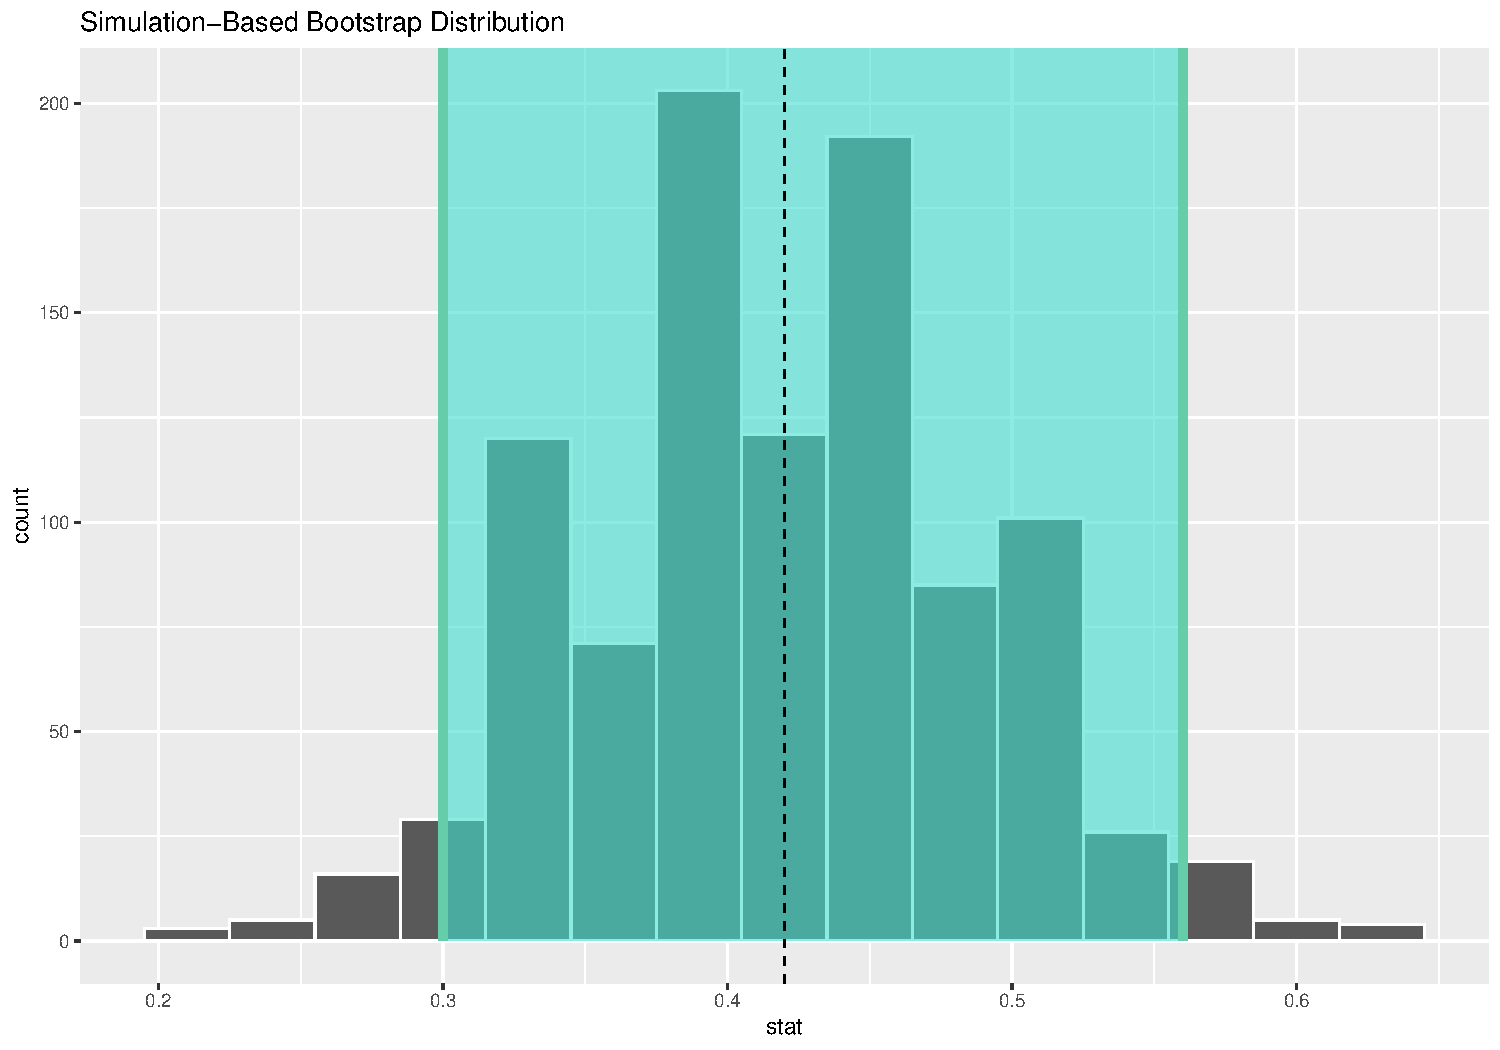
\includegraphics[width=0.7\linewidth,height=0.45\textheight]{Week10_Lect_files/figure-beamer/unnamed-chunk-25-1} \end{center}
\normalsize

In this case the \(95\%\) confidence interval for \(p\), (0.3, 0.56),
contains the true value of 0.375.
\end{frame}

\begin{frame}{Interpreting confidence intervals: Sampling bowl example}
\protect\hypertarget{interpreting-confidence-intervals-sampling-bowl-example}{}
\begin{itemize}
\item
  However, will every \(95\%\) confidence interval for \(p\) capture
  this value?
\item
  Let's now repeat this process 100 more times: we take 100 virtual
  samples from the bowl and construct 100 \(95\%\) confidence intervals.
\end{itemize}

\tiny

\begin{center}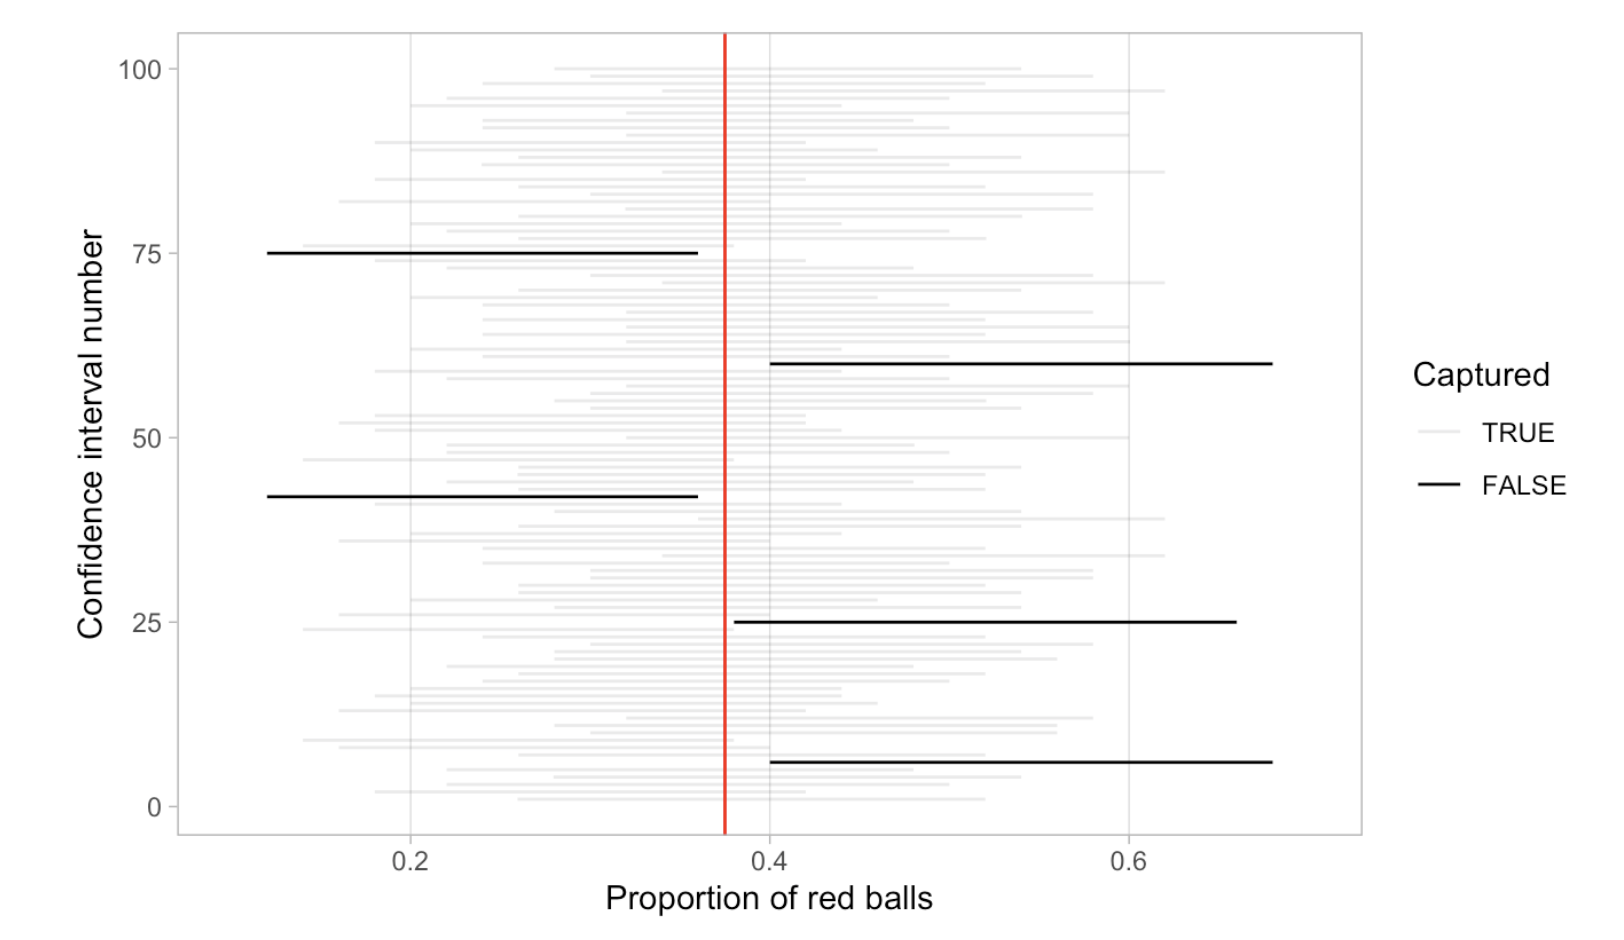
\includegraphics[width=0.6\linewidth,height=0.4\textheight]{week10_11} \end{center}
\normalsize

\begin{itemize}
\item
  Of the 100 \(95\%\) confidence intervals, 95 of them captured the true
  value \(p=0.375\), whereas 5 of them didn't.

  \begin{itemize}
  \tightlist
  \item
    This is where the ``\(95\%\) confidence level'' comes into play.
  \end{itemize}
\end{itemize}
\end{frame}

\begin{frame}{Interpreting confidence intervals: Sampling bowl example}
\protect\hypertarget{interpreting-confidence-intervals-sampling-bowl-example-1}{}
\begin{itemize}
\tightlist
\item
  Below is a graph for 100 \(80\%\) confidence intervals.
\end{itemize}

\tiny

\begin{center}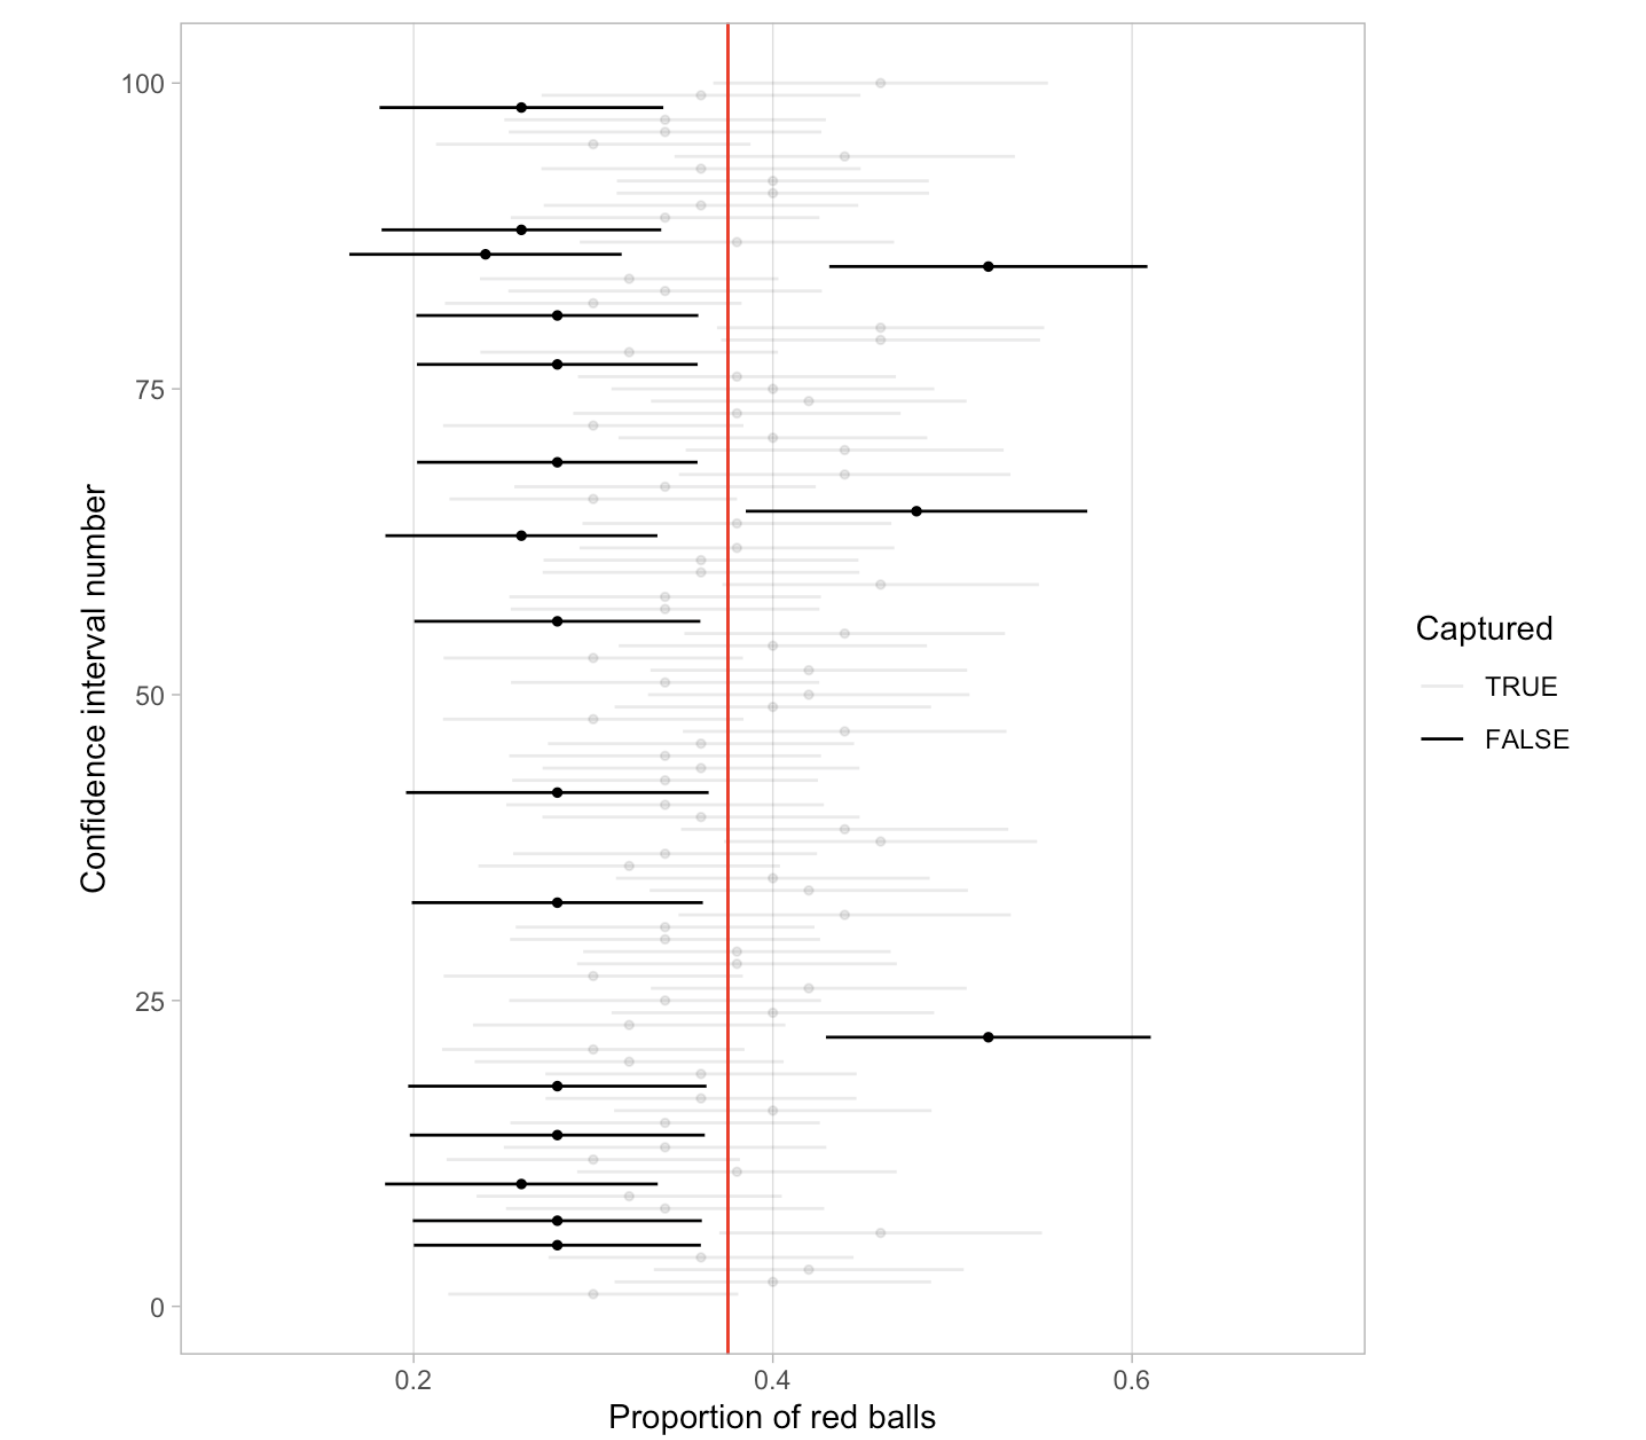
\includegraphics[width=0.6\linewidth,height=0.5\textheight]{week10_12} \end{center}
\normalsize

\begin{itemize}
\tightlist
\item
  Of the 100 \(80\%\) confidence intervals, 82 of them captured the true
  value \(p=0.375\), whereas 18 of them didn't.
\end{itemize}
\end{frame}

\begin{frame}{Interpreting confidence intervals}
\protect\hypertarget{interpreting-confidence-intervals-4}{}
The precise and mathematically correct interpretation of a \(95\%\)
confidence interval is a little long-winded:

\begin{tcolorbox}
Precise interpretation: If we repeated our sampling procedure a large number of times, we expect about $95\%$ of the resulting confidence intervals to capture the value of the population parameter.
\end{tcolorbox}

The shorthand summary of the precise interpretation:

\begin{tcolorbox}
Short-hand interpretation: We are $95\%$ “confident” that a $95\%$ confidence interval captures the value of the population parameter.
\end{tcolorbox}
\end{frame}

\begin{frame}{Width of confidence intervals}
\protect\hypertarget{width-of-confidence-intervals}{}
Let's go over some factors that determine their width.

\begin{enumerate}
\item
  Impact of confidence level.
\item
  Impact of sample size.
\end{enumerate}
\end{frame}

\hypertarget{two-sample-boostrap}{%
\section{Two Sample Boostrap}\label{two-sample-boostrap}}

\begin{frame}{Two Sample Boostrap}
\protect\hypertarget{two-sample-boostrap-1}{}
We now turn to the problem of comparing two samples.

\begin{itemize}
\item
  In general, bootstrapping should mimic how the data were obtained.

  \begin{itemize}
  \tightlist
  \item
    So the data correspond to independent samples from two populations,
    we should draw the samples that way.
  \end{itemize}
\item
  Then we proceed to compute the same statistic comparing the samples as
  per the original data, for example, difference in means or ratio of
  proportions.
\end{itemize}
\end{frame}

\begin{frame}{Two Sample Boostrap}
\protect\hypertarget{two-sample-boostrap-2}{}
Given independent samples of sizes \(m\) and \(n\) from two populations,

\begin{enumerate}
\item
  Draw a resample of size \(m\) with replacement from the first sample
  and a separate resample of size \(n\) for the second sample. Compute a
  statistic that compares the two groups, such as the difference between
  the two sample means.
\item
  Repeat this resampling process many times say 10,000.
\item
  Construct the bootstrap distribution of the statistic. Inspect its
  spread, bias, and shape.
\end{enumerate}
\end{frame}

\begin{frame}[fragile]{TV example}
\protect\hypertarget{tv-example}{}
\begin{tcolorbox}
A high school student was curious about the total number of minutes devoted to commercials during any given half-hour time period on basic and extended cable TV channels.
\end{tcolorbox}

Lets use the \texttt{TV} dataset from the \texttt{resampledata} package.
\small

\begin{Shaded}
\begin{Highlighting}[]
\FunctionTok{library}\NormalTok{(resampledata)}
\FunctionTok{library}\NormalTok{(tidyverse)}
\FunctionTok{library}\NormalTok{(moderndive)}
\FunctionTok{library}\NormalTok{(infer)}
\FunctionTok{head}\NormalTok{(TV)}
\end{Highlighting}
\end{Shaded}

\begin{verbatim}
  ID Times Cable
1  1   7.0 Basic
2  2  10.0 Basic
3  3  10.6 Basic
4  4  10.2 Basic
5  5   8.6 Basic
6  6   7.6 Basic
\end{verbatim}

\normalsize
\end{frame}

\begin{frame}[fragile]{TV example}
\protect\hypertarget{tv-example-1}{}
\small

\begin{Shaded}
\begin{Highlighting}[]
\NormalTok{ct }\OtherTok{\textless{}{-}} \FunctionTok{tapply}\NormalTok{(TV}\SpecialCharTok{$}\NormalTok{Times, TV}\SpecialCharTok{$}\NormalTok{Cable, mean)}
\NormalTok{ct}
\end{Highlighting}
\end{Shaded}

\begin{verbatim}
   Basic Extended 
    9.21     6.87 
\end{verbatim}

\begin{Shaded}
\begin{Highlighting}[]
\CommentTok{\# Tidy approach}
\NormalTok{TV }\SpecialCharTok{\%\textgreater{}\%}
  \FunctionTok{group\_by}\NormalTok{(Cable) }\SpecialCharTok{\%\textgreater{}\%}
  \FunctionTok{summarize}\NormalTok{(}\AttributeTok{Means =} \FunctionTok{mean}\NormalTok{(Times), }\AttributeTok{n =} \FunctionTok{n}\NormalTok{())}
\end{Highlighting}
\end{Shaded}

\begin{verbatim}
# A tibble: 2 x 3
  Cable    Means     n
  <fct>    <dbl> <int>
1 Basic     9.21    10
2 Extended  6.87    10
\end{verbatim}

\normalsize

\begin{itemize}
\item
  The means of the basic and extended channel commercial times are 9.21
  and 6.87 min.
\item
  Is this difference of 2.34 min. statistically significant?
\end{itemize}
\end{frame}

\begin{frame}{TV example}
\protect\hypertarget{tv-example-2}{}
\begin{itemize}
\item
  The original data are simple random samples of size 10 from two
  populations.

  \begin{itemize}
  \tightlist
  \item
    We draw a bootstrap sample from the basic channel data and
    independently draw a bootstrap sample from the extended channel
    data,
  \item
    compute the means for each sample, and take the difference.
  \end{itemize}
\end{itemize}
\end{frame}

\begin{frame}[fragile]{TV example}
\protect\hypertarget{tv-example-3}{}
\tiny

\begin{Shaded}
\begin{Highlighting}[]
\NormalTok{times.Basic }\OtherTok{\textless{}{-}} \FunctionTok{subset}\NormalTok{(TV, }\AttributeTok{select =}\NormalTok{ Times, }
                      \AttributeTok{subset =}\NormalTok{ Cable }\SpecialCharTok{==} \StringTok{"Basic"}\NormalTok{, }\AttributeTok{drop =} \ConstantTok{TRUE}\NormalTok{)}
\NormalTok{times.Ext }\OtherTok{\textless{}{-}} \FunctionTok{subset}\NormalTok{(TV, }\AttributeTok{select =}\NormalTok{ Times, }
                    \AttributeTok{subset =}\NormalTok{ Cable }\SpecialCharTok{==} \StringTok{"Extended"}\NormalTok{, }\AttributeTok{drop =} \ConstantTok{TRUE}\NormalTok{)}
\NormalTok{B }\OtherTok{\textless{}{-}} \DecValTok{10}\SpecialCharTok{\^{}}\DecValTok{4}
\NormalTok{times.diff.mean }\OtherTok{\textless{}{-}} \FunctionTok{numeric}\NormalTok{(B)}
\FunctionTok{set.seed}\NormalTok{(}\DecValTok{5}\NormalTok{)}
\ControlFlowTok{for}\NormalTok{ (i }\ControlFlowTok{in} \DecValTok{1}\SpecialCharTok{:}\NormalTok{B)\{}
\NormalTok{  Basic.sample }\OtherTok{\textless{}{-}} \FunctionTok{sample}\NormalTok{(times.Basic, }
                  \AttributeTok{size =} \FunctionTok{sum}\NormalTok{(}\SpecialCharTok{!}\FunctionTok{is.na}\NormalTok{(times.Basic)), }\AttributeTok{replace =} \ConstantTok{TRUE}\NormalTok{)}
\NormalTok{  Ext.sample }\OtherTok{\textless{}{-}} \FunctionTok{sample}\NormalTok{(times.Ext,}
                  \AttributeTok{size =} \FunctionTok{sum}\NormalTok{(}\SpecialCharTok{!}\FunctionTok{is.na}\NormalTok{(times.Ext)), }\AttributeTok{replace =} \ConstantTok{TRUE}\NormalTok{)}
\NormalTok{  times.diff.mean[i] }\OtherTok{\textless{}{-}} \FunctionTok{mean}\NormalTok{(Basic.sample) }\SpecialCharTok{{-}} \FunctionTok{mean}\NormalTok{(Ext.sample)}
\NormalTok{\}}
\NormalTok{opar }\OtherTok{\textless{}{-}} \FunctionTok{par}\NormalTok{(}\AttributeTok{no.readonly =} \ConstantTok{TRUE}\NormalTok{)}
\FunctionTok{par}\NormalTok{(}\AttributeTok{mfrow=}\FunctionTok{c}\NormalTok{(}\DecValTok{1}\NormalTok{, }\DecValTok{2}\NormalTok{))}
\NormalTok{CI }\OtherTok{\textless{}{-}} \FunctionTok{quantile}\NormalTok{(times.diff.mean, }\AttributeTok{prob =} \FunctionTok{c}\NormalTok{(}\FloatTok{0.025}\NormalTok{, }\FloatTok{0.975}\NormalTok{))}
\NormalTok{CI}
\end{Highlighting}
\end{Shaded}

\begin{verbatim}
 2.5% 97.5% 
 0.90  3.86 
\end{verbatim}

\normalsize
\end{frame}

\begin{frame}[fragile]{TV example}
\protect\hypertarget{tv-example-4}{}
\tiny

\begin{Shaded}
\begin{Highlighting}[]
\FunctionTok{par}\NormalTok{(}\AttributeTok{mfrow =} \FunctionTok{c}\NormalTok{(}\DecValTok{1}\NormalTok{, }\DecValTok{2}\NormalTok{))}
\FunctionTok{hist}\NormalTok{(times.diff.mean, }\AttributeTok{breaks =} \StringTok{"Scott"}\NormalTok{, }\AttributeTok{freq=}\ConstantTok{FALSE}\NormalTok{, }
     \AttributeTok{main =} \StringTok{"Bootstrap Distribution }\SpecialCharTok{\textbackslash{}n}\StringTok{ (Figure a)"}\NormalTok{, }
     \AttributeTok{xlab =} \FunctionTok{substitute}\NormalTok{(}\FunctionTok{paste}\NormalTok{(}\FunctionTok{bar}\NormalTok{(x)[}\DecValTok{1}\NormalTok{],}\StringTok{"*"}\NormalTok{, }\SpecialCharTok{{-}} \FunctionTok{bar}\NormalTok{(x)[}\DecValTok{2}\NormalTok{],}\StringTok{"*"}\NormalTok{)), }
     \AttributeTok{col =} \StringTok{"lightblue"}\NormalTok{)}
\FunctionTok{abline}\NormalTok{(}\AttributeTok{v =} \FunctionTok{c}\NormalTok{(}\DecValTok{0}\NormalTok{, CI), }\AttributeTok{col =} \FunctionTok{c}\NormalTok{(}\StringTok{"blue"}\NormalTok{, }\StringTok{"red"}\NormalTok{, }\StringTok{"red"}\NormalTok{), }\AttributeTok{lwd =} \DecValTok{2}\NormalTok{, }
       \AttributeTok{lty =} \FunctionTok{c}\NormalTok{(}\StringTok{"solid"}\NormalTok{, }\StringTok{"dashed"}\NormalTok{, }\StringTok{"dashed"}\NormalTok{))}
\FunctionTok{qqnorm}\NormalTok{(times.diff.mean, }\AttributeTok{main =} \StringTok{"Normal Q{-}Q Plot }\SpecialCharTok{\textbackslash{}n}\StringTok{ (Figure b)"}\NormalTok{)}
\FunctionTok{qqline}\NormalTok{(times.diff.mean, }\AttributeTok{col =} \StringTok{"red"}\NormalTok{)}
\end{Highlighting}
\end{Shaded}

\begin{center}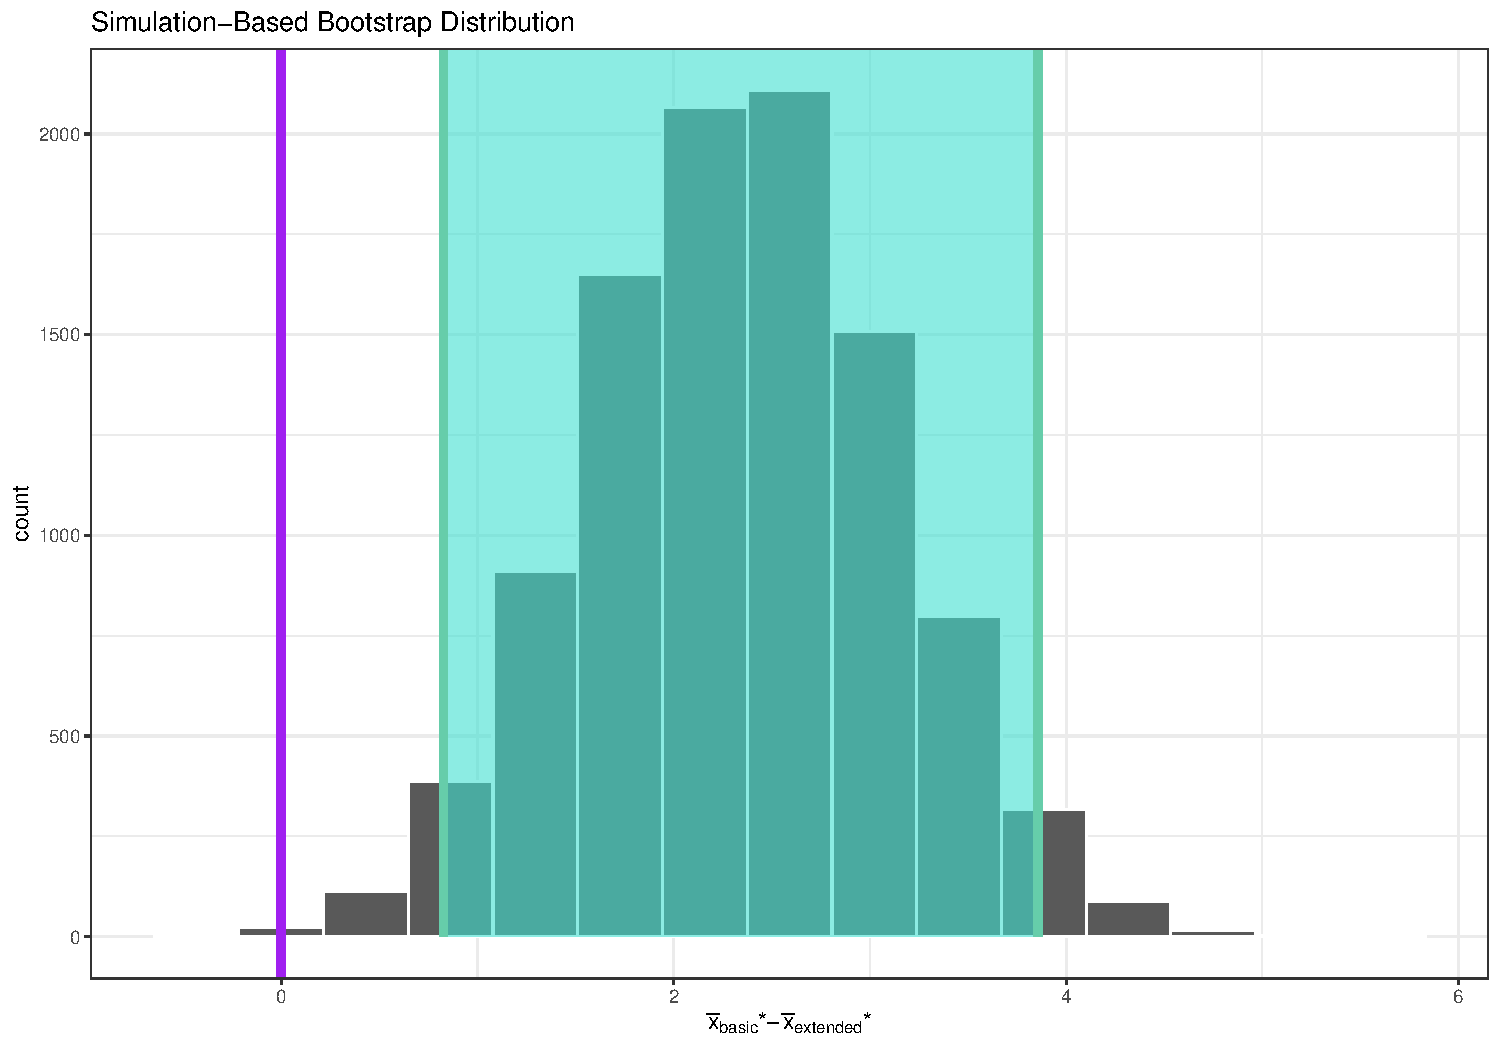
\includegraphics[width=0.7\linewidth,height=0.43\textheight]{Week10_Lect_files/figure-beamer/unnamed-chunk-31-1} \end{center}

\begin{Shaded}
\begin{Highlighting}[]
\FunctionTok{sd}\NormalTok{(times.diff.mean) }\OtherTok{{-}\textgreater{}}\NormalTok{ SEbdm}
\NormalTok{SEbdm}
\end{Highlighting}
\end{Shaded}

\begin{verbatim}
[1] 0.7552861
\end{verbatim}

\normalsize
\end{frame}

\begin{frame}{TV example}
\protect\hypertarget{tv-example-5}{}
\begin{itemize}
\item
  Figure a shows the bootstrap distribution of the difference of sample
  means.

  \begin{itemize}
  \tightlist
  \item
    As in the single sample case, we see that the bootstrap distribution
    is approximately normal and centered at the original statistics (the
    difference in sample means).
  \item
    We also get a quick idea of how much the difference in sample means
    varies due to random sampling.
  \item
    We may quantify this variation by computing the bootstrap standard
    error, which is 0.7552861. Again, the bootstrap standard error is
    the standard error of the sampling distribution.
  \end{itemize}
\item
  The right panel of Figure b shows a normal-quantile plot for the
  bootstrap distribution: the distribution is very close to normal.
\item
  The \(95\%\) bootstrap percentile confidence interval for the
  difference in means (basic- extended) is (0.9, 3.86).

  \begin{itemize}
  \tightlist
  \item
    Thus, we are \(95\%\) confident that commercial times on basic
    channels are, on average, between 0.9 and 3.86 min.
  \item
    longer than on extended channels (per half-hour time periods).
  \end{itemize}
\end{itemize}
\end{frame}

\begin{frame}[fragile]{TV example}
\protect\hypertarget{tv-example-6}{}
Using the \texttt{infer} pipeline

\tiny

\begin{Shaded}
\begin{Highlighting}[]
\FunctionTok{set.seed}\NormalTok{(}\DecValTok{5}\NormalTok{)}
\NormalTok{TV }\SpecialCharTok{\%\textgreater{}\%} 
  \FunctionTok{specify}\NormalTok{(Times }\SpecialCharTok{\textasciitilde{}}\NormalTok{ Cable) }\SpecialCharTok{\%\textgreater{}\%} 
  \FunctionTok{generate}\NormalTok{(}\AttributeTok{reps =} \DecValTok{10}\SpecialCharTok{\^{}}\DecValTok{4} \SpecialCharTok{{-}} \DecValTok{1}\NormalTok{, }\AttributeTok{type =} \StringTok{"bootstrap"}\NormalTok{) }\SpecialCharTok{\%\textgreater{}\%} 
  \FunctionTok{calculate}\NormalTok{(}\AttributeTok{stat =} \StringTok{"diff in means"}\NormalTok{, }\AttributeTok{order =} \FunctionTok{c}\NormalTok{(}\StringTok{"Basic"}\NormalTok{, }\StringTok{"Extended"}\NormalTok{)) }\OtherTok{{-}\textgreater{}}\NormalTok{ bootdist}
\FunctionTok{visualize}\NormalTok{(bootdist) }\SpecialCharTok{+} \FunctionTok{theme\_bw}\NormalTok{() }\SpecialCharTok{+}
  \FunctionTok{labs}\NormalTok{(}\AttributeTok{x =} \FunctionTok{substitute}\NormalTok{(}\FunctionTok{paste}\NormalTok{(}\FunctionTok{bar}\NormalTok{(x)[basic],}\StringTok{"*"}\NormalTok{, }\SpecialCharTok{{-}} \FunctionTok{bar}\NormalTok{(x)[extended],}\StringTok{"*"}\NormalTok{)))}
\end{Highlighting}
\end{Shaded}

\begin{center}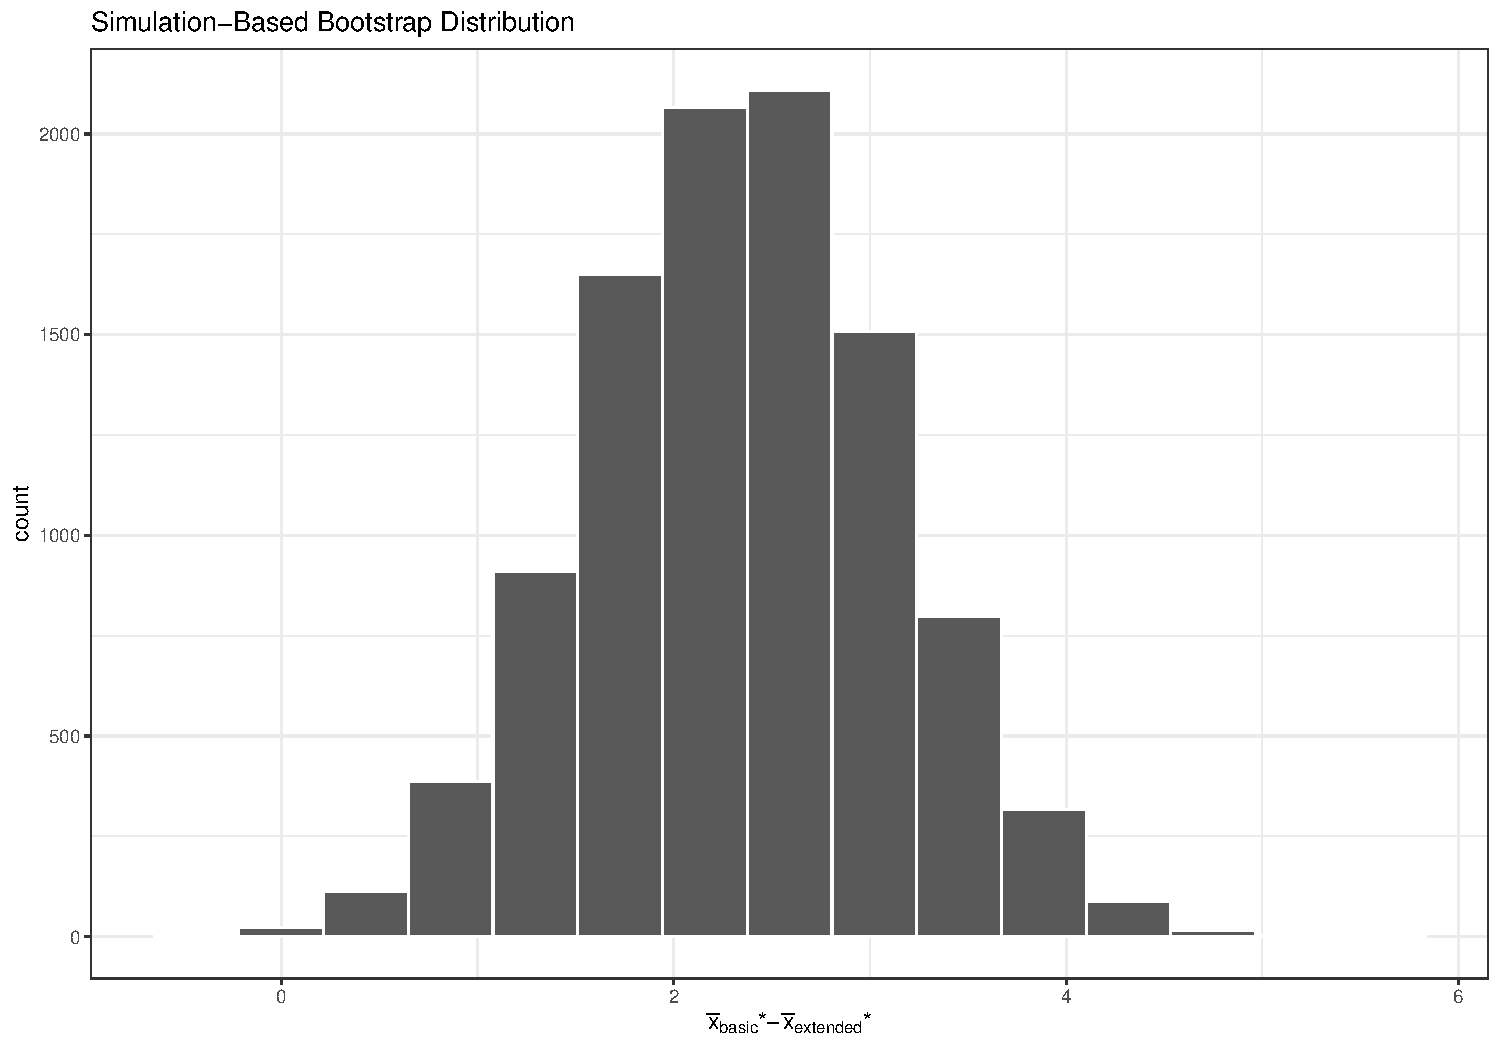
\includegraphics[width=0.7\linewidth,height=0.45\textheight]{Week10_Lect_files/figure-beamer/unnamed-chunk-32-1} \end{center}
\normalsize
\end{frame}

\begin{frame}[fragile]{TV example}
\protect\hypertarget{tv-example-7}{}
Using the \texttt{infer} pipeline

\tiny

\begin{Shaded}
\begin{Highlighting}[]
\FunctionTok{get\_confidence\_interval}\NormalTok{(bootdist, }\AttributeTok{level =} \FloatTok{0.95}\NormalTok{) }\OtherTok{{-}\textgreater{}}\NormalTok{ CI2}
\NormalTok{CI2}
\end{Highlighting}
\end{Shaded}

\begin{verbatim}
# A tibble: 1 x 2
  lower_ci upper_ci
     <dbl>    <dbl>
1    0.827     3.85
\end{verbatim}

\begin{Shaded}
\begin{Highlighting}[]
\DocumentationTok{\#\#\#}
\FunctionTok{visualize}\NormalTok{(bootdist) }\SpecialCharTok{+} \FunctionTok{theme\_bw}\NormalTok{() }\SpecialCharTok{+}
  \FunctionTok{labs}\NormalTok{(}\AttributeTok{x =} \FunctionTok{substitute}\NormalTok{(}\FunctionTok{paste}\NormalTok{(}\FunctionTok{bar}\NormalTok{(x)[basic],}\StringTok{"*"}\NormalTok{, }\SpecialCharTok{{-}} \FunctionTok{bar}\NormalTok{(x)[extended],}\StringTok{"*"}\NormalTok{))) }\SpecialCharTok{+} 
  \FunctionTok{shade\_confidence\_interval}\NormalTok{(}\AttributeTok{endpoints =}\NormalTok{ CI2) }\SpecialCharTok{+} 
  \FunctionTok{geom\_vline}\NormalTok{(}\AttributeTok{xintercept =} \DecValTok{0}\NormalTok{, }\AttributeTok{color =} \StringTok{"purple"}\NormalTok{, }\AttributeTok{size =} \DecValTok{2}\NormalTok{)}
\end{Highlighting}
\end{Shaded}

\begin{center}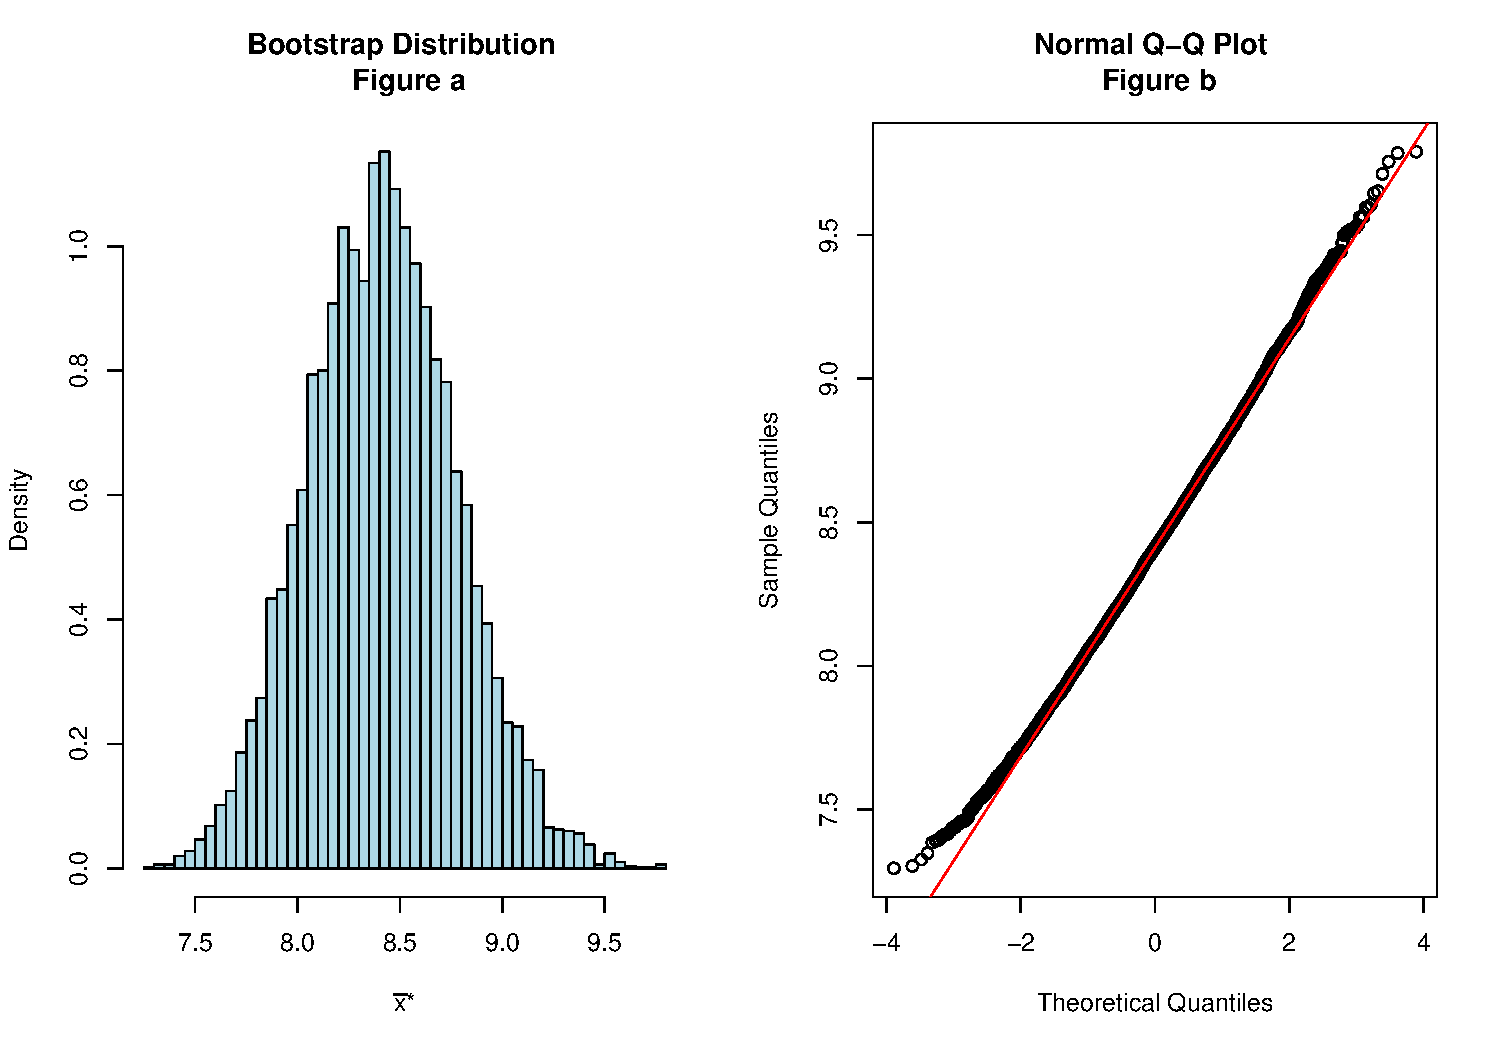
\includegraphics[width=0.6\linewidth,height=0.38\textheight]{Week10_Lect_files/figure-beamer/unnamed-chunk-33-1} \end{center}
\normalsize
\end{frame}

\begin{frame}{Verizon example}
\protect\hypertarget{verizon-example}{}
\begin{tcolorbox}
Verizon is the primary local telephone company (incumbent local exchange carrier, ILEC) for a large area of the eastern United States. As such it is responsible for providing repair service for the customers of other telephone companies known as competing local exchange carriers (CLECs) in this region. Verizon is subject to fines if the repair times (the time it takes to fix a problem) for CLEC customers are substantially worse than those for Verizon customers. The data set Verizon contains a random sample of repair times for 1664 ILEC and 23 CLEC customers.
\end{tcolorbox}
\end{frame}

\begin{frame}[fragile]{Verizon example}
\protect\hypertarget{verizon-example-1}{}
\normalsize

\begin{Shaded}
\begin{Highlighting}[]
\NormalTok{Phone }\OtherTok{\textless{}{-}}\NormalTok{ Verizon}
\NormalTok{rt }\OtherTok{\textless{}{-}} \FunctionTok{tapply}\NormalTok{(Phone}\SpecialCharTok{$}\NormalTok{Time, Phone}\SpecialCharTok{$}\NormalTok{Group, mean)}
\NormalTok{rt}
\end{Highlighting}
\end{Shaded}

\begin{verbatim}
     CLEC      ILEC 
16.509130  8.411611 
\end{verbatim}

\begin{Shaded}
\begin{Highlighting}[]
\CommentTok{\# Tidy approach}
\NormalTok{Phone }\SpecialCharTok{\%\textgreater{}\%} 
  \FunctionTok{group\_by}\NormalTok{(Group) }\SpecialCharTok{\%\textgreater{}\%} 
  \FunctionTok{summarize}\NormalTok{(}\AttributeTok{Mean =} \FunctionTok{mean}\NormalTok{(Time), }\AttributeTok{n =} \FunctionTok{n}\NormalTok{(), }\AttributeTok{SD =} \FunctionTok{sd}\NormalTok{(Time))}
\end{Highlighting}
\end{Shaded}

\begin{verbatim}
# A tibble: 2 x 4
  Group  Mean     n    SD
  <fct> <dbl> <int> <dbl>
1 CLEC  16.5     23  19.5
2 ILEC   8.41  1664  14.7
\end{verbatim}

\normalsize
\end{frame}

\begin{frame}[fragile]{Verizon example}
\protect\hypertarget{verizon-example-2}{}
\tiny

\begin{Shaded}
\begin{Highlighting}[]
\FunctionTok{par}\NormalTok{(}\AttributeTok{mfrow =} \FunctionTok{c}\NormalTok{(}\DecValTok{1}\NormalTok{, }\DecValTok{2}\NormalTok{))}
\NormalTok{times.ILEC }\OtherTok{\textless{}{-}} \FunctionTok{subset}\NormalTok{(Phone, }\AttributeTok{select =}\NormalTok{ Time, }\AttributeTok{subset =}\NormalTok{ Group }\SpecialCharTok{==} \StringTok{"ILEC"}\NormalTok{, }\AttributeTok{drop =} \ConstantTok{TRUE}\NormalTok{)}
\NormalTok{B }\OtherTok{\textless{}{-}} \DecValTok{10}\SpecialCharTok{\^{}}\DecValTok{4}
\NormalTok{ILECmean }\OtherTok{\textless{}{-}} \FunctionTok{numeric}\NormalTok{(B)}
\FunctionTok{set.seed}\NormalTok{(}\DecValTok{3}\NormalTok{)}
\ControlFlowTok{for}\NormalTok{ (i }\ControlFlowTok{in} \DecValTok{1}\SpecialCharTok{:}\NormalTok{B)\{}
\NormalTok{ ILECmean[i] }\OtherTok{\textless{}{-}} \FunctionTok{mean}\NormalTok{(}\FunctionTok{sample}\NormalTok{(times.ILEC, }\AttributeTok{size =} \FunctionTok{length}\NormalTok{(times.ILEC), }\AttributeTok{replace =} \ConstantTok{TRUE}\NormalTok{)) }
\NormalTok{\}}
\NormalTok{opar }\OtherTok{\textless{}{-}} \FunctionTok{par}\NormalTok{(}\AttributeTok{no.readonly =} \ConstantTok{TRUE}\NormalTok{)}
\FunctionTok{par}\NormalTok{(}\AttributeTok{mfrow=}\FunctionTok{c}\NormalTok{(}\DecValTok{1}\NormalTok{, }\DecValTok{2}\NormalTok{))}
\FunctionTok{hist}\NormalTok{(ILECmean, }\AttributeTok{breaks =} \StringTok{"Scott"}\NormalTok{, }\AttributeTok{col =} \StringTok{"lightblue"}\NormalTok{, }
     \AttributeTok{main =} \StringTok{"Bootstrap Distribution }\SpecialCharTok{\textbackslash{}n}\StringTok{ Figure a"}\NormalTok{, }
     \AttributeTok{freq=} \ConstantTok{FALSE}\NormalTok{, }\AttributeTok{xlab =} \FunctionTok{substitute}\NormalTok{(}\FunctionTok{paste}\NormalTok{(}\FunctionTok{bar}\NormalTok{(x),}\StringTok{"*"}\NormalTok{)))}
\FunctionTok{qqnorm}\NormalTok{(ILECmean, }\AttributeTok{main =} \StringTok{"Normal Q{-}Q Plot }\SpecialCharTok{\textbackslash{}n}\StringTok{ Figure b"}\NormalTok{)}
\FunctionTok{qqline}\NormalTok{(ILECmean, }\AttributeTok{col =} \StringTok{"red"}\NormalTok{)}
\end{Highlighting}
\end{Shaded}

\begin{center}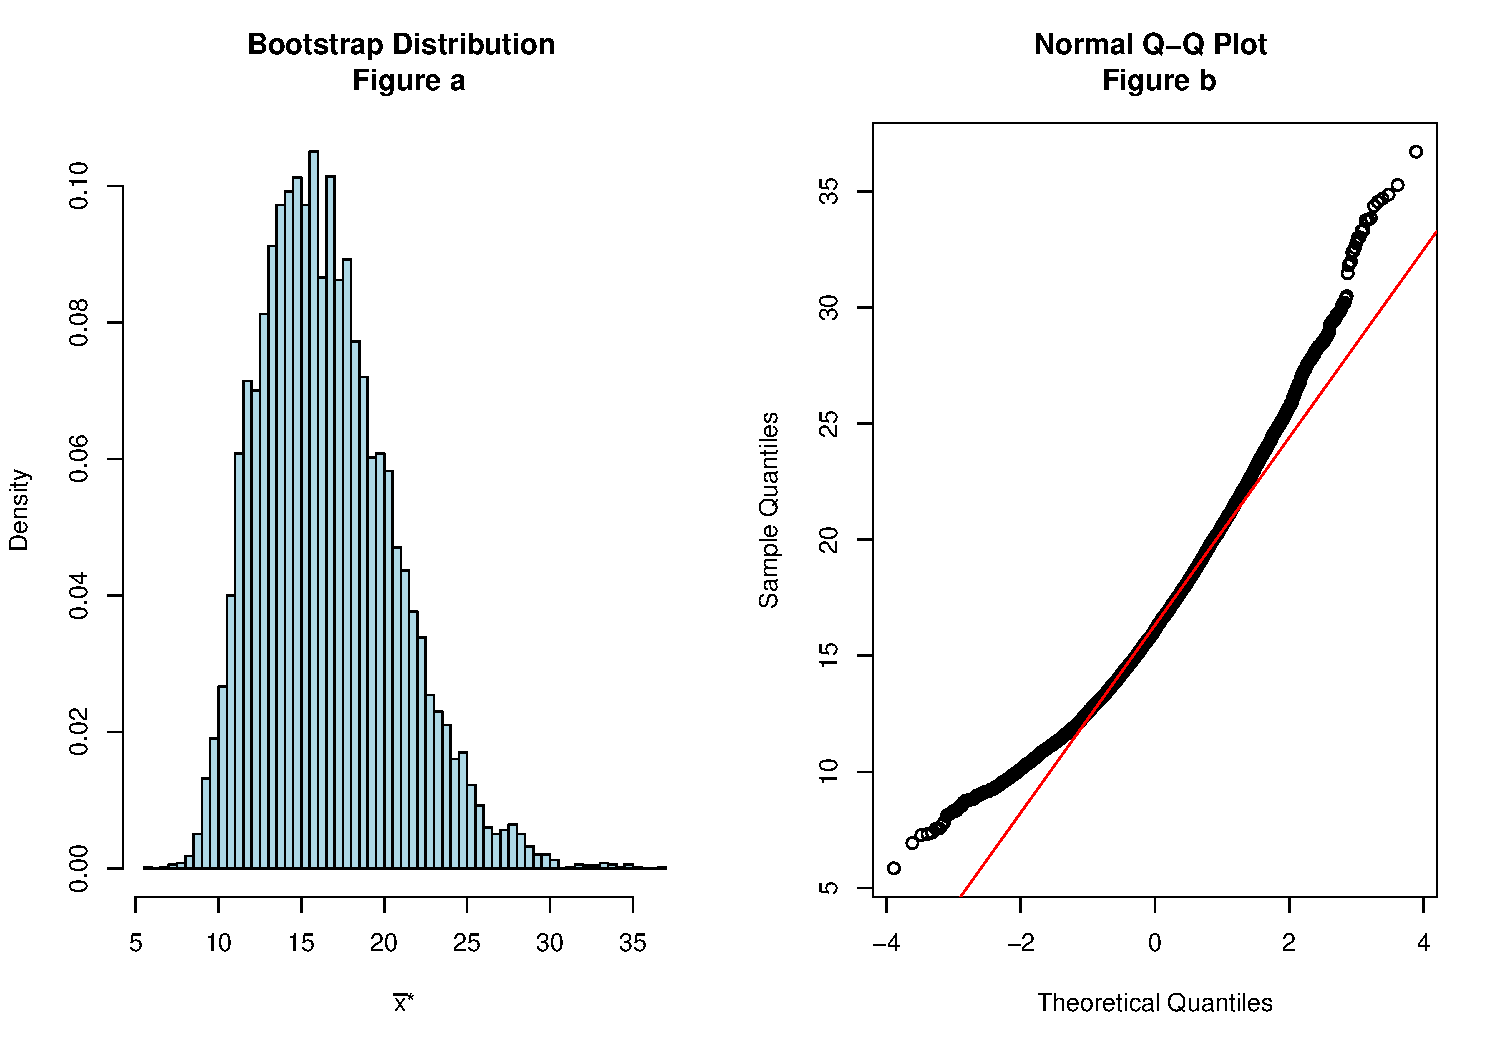
\includegraphics[width=0.6\linewidth,height=0.4\textheight]{Week10_Lect_files/figure-beamer/unnamed-chunk-35-1} \end{center}
\normalsize
\end{frame}

\begin{frame}[fragile]{Verizon example}
\protect\hypertarget{verizon-example-3}{}
\begin{itemize}
\item
  The bootstrap distribution for the larger ILEC data set (\(n=1664\))
  is shown in Figure a.

  \begin{itemize}
  \tightlist
  \item
    The distribution is centered around the sample mean of 8.4151654,
  \item
    has a relatively narrow spread primarily due to the large sample
    size,
  \item
    with the bootstrap standard error of 0.361873 and
  \item
    a \(95\%\) bootstrap percentile interval of (7.725662, 9.1467858).
  \item
    The distribution is roughly symmetric, with little skewness.
  \end{itemize}
\end{itemize}

\small

\begin{Shaded}
\begin{Highlighting}[]
\FunctionTok{sd}\NormalTok{(ILECmean)}
\end{Highlighting}
\end{Shaded}

\begin{verbatim}
[1] 0.361873
\end{verbatim}

\begin{Shaded}
\begin{Highlighting}[]
\NormalTok{CI }\OtherTok{\textless{}{-}} \FunctionTok{quantile}\NormalTok{(ILECmean, }\AttributeTok{prob =} \FunctionTok{c}\NormalTok{(}\FloatTok{0.025}\NormalTok{, }\FloatTok{0.975}\NormalTok{))}
\NormalTok{CI}
\end{Highlighting}
\end{Shaded}

\begin{verbatim}
    2.5%    97.5% 
7.725662 9.146786 
\end{verbatim}

\normalsize
\end{frame}

\begin{frame}[fragile]{Verizon example}
\protect\hypertarget{verizon-example-4}{}
The bootstrap distribution for the smaller CLEC data set (n=23)

\tiny

\begin{Shaded}
\begin{Highlighting}[]
\FunctionTok{par}\NormalTok{(}\AttributeTok{mfrow =} \FunctionTok{c}\NormalTok{(}\DecValTok{1}\NormalTok{, }\DecValTok{2}\NormalTok{))}
\NormalTok{times.CLEC }\OtherTok{\textless{}{-}} \FunctionTok{subset}\NormalTok{(Phone, }\AttributeTok{select =}\NormalTok{ Time, }\AttributeTok{subset =}\NormalTok{ Group }\SpecialCharTok{==} \StringTok{"CLEC"}\NormalTok{, }\AttributeTok{drop =} \ConstantTok{TRUE}\NormalTok{)}
\NormalTok{B }\OtherTok{\textless{}{-}} \DecValTok{10}\SpecialCharTok{\^{}}\DecValTok{4}
\NormalTok{CLECmean }\OtherTok{\textless{}{-}} \FunctionTok{numeric}\NormalTok{(B)}
\FunctionTok{set.seed}\NormalTok{(}\DecValTok{2}\NormalTok{)}
\ControlFlowTok{for}\NormalTok{ (i }\ControlFlowTok{in} \DecValTok{1}\SpecialCharTok{:}\NormalTok{B)\{}
\NormalTok{ CLECmean[i] }\OtherTok{\textless{}{-}} \FunctionTok{mean}\NormalTok{(}\FunctionTok{sample}\NormalTok{(times.CLEC, }\AttributeTok{size =} \FunctionTok{length}\NormalTok{(times.CLEC), }\AttributeTok{replace =} \ConstantTok{TRUE}\NormalTok{)) }
\NormalTok{\}}
\NormalTok{opar }\OtherTok{\textless{}{-}} \FunctionTok{par}\NormalTok{(}\AttributeTok{no.readonly =} \ConstantTok{TRUE}\NormalTok{)}
\FunctionTok{par}\NormalTok{(}\AttributeTok{mfrow=}\FunctionTok{c}\NormalTok{(}\DecValTok{1}\NormalTok{, }\DecValTok{2}\NormalTok{))}
\FunctionTok{hist}\NormalTok{(CLECmean, }\AttributeTok{breaks =} \StringTok{"Scott"}\NormalTok{, }\AttributeTok{col =} \StringTok{"lightblue"}\NormalTok{, }
     \AttributeTok{main =} \StringTok{"Bootstrap Distribution }\SpecialCharTok{\textbackslash{}n}\StringTok{ Figure a"}\NormalTok{, }
     \AttributeTok{freq=} \ConstantTok{FALSE}\NormalTok{, }\AttributeTok{xlab =} \FunctionTok{substitute}\NormalTok{(}\FunctionTok{paste}\NormalTok{(}\FunctionTok{bar}\NormalTok{(x),}\StringTok{"*"}\NormalTok{)))}
\FunctionTok{qqnorm}\NormalTok{(CLECmean, }\AttributeTok{main =} \StringTok{"Normal Q{-}Q Plot }\SpecialCharTok{\textbackslash{}n}\StringTok{ Figure b"}\NormalTok{)}
\FunctionTok{qqline}\NormalTok{(CLECmean, }\AttributeTok{col =} \StringTok{"red"}\NormalTok{)}
\end{Highlighting}
\end{Shaded}

\begin{center}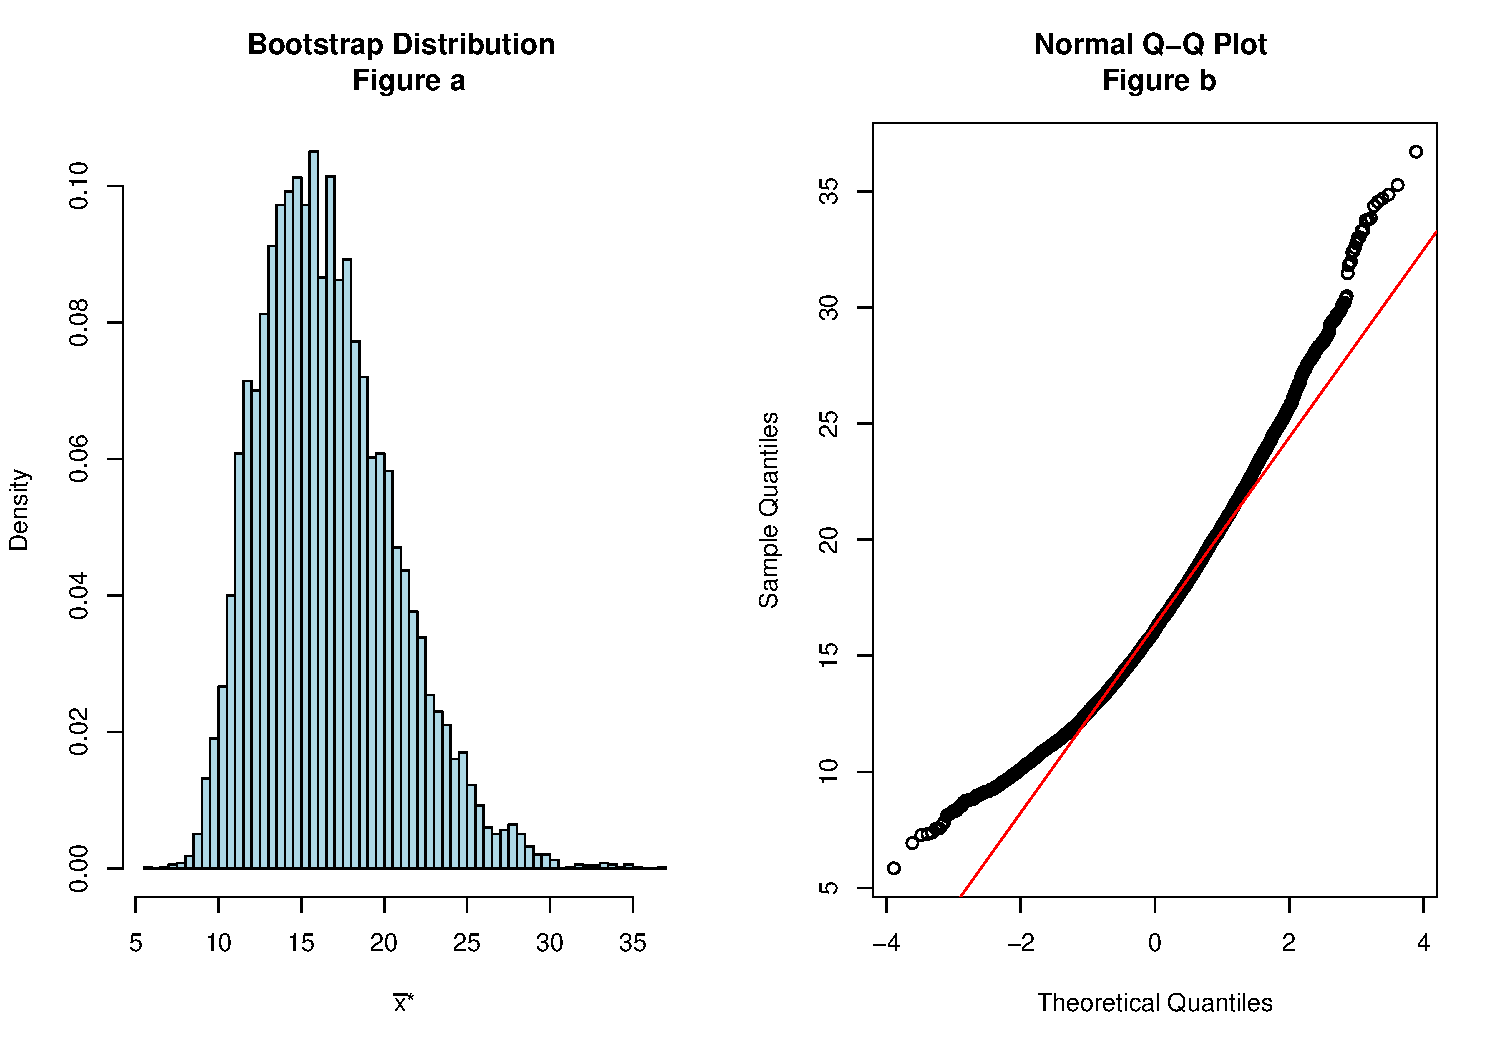
\includegraphics[width=0.6\linewidth,height=0.35\textheight]{Week10_Lect_files/figure-beamer/unnamed-chunk-37-1} \end{center}
\normalsize
\end{frame}

\begin{frame}[fragile]{Verizon example}
\protect\hypertarget{verizon-example-5}{}
\begin{itemize}
\tightlist
\item
  The bootstrap distribution for the smaller CLEC data set (n=23) is
  shown in Figure a.
\end{itemize}

\small

\begin{Shaded}
\begin{Highlighting}[]
\FunctionTok{c}\NormalTok{(}\FunctionTok{sd}\NormalTok{(CLECmean), }\FunctionTok{mean}\NormalTok{(CLECmean))}
\end{Highlighting}
\end{Shaded}

\begin{verbatim}
[1]  4.022913 16.572639
\end{verbatim}

\begin{Shaded}
\begin{Highlighting}[]
\NormalTok{CIC }\OtherTok{\textless{}{-}} \FunctionTok{quantile}\NormalTok{(CLECmean, }\AttributeTok{prob =} \FunctionTok{c}\NormalTok{(}\FloatTok{0.025}\NormalTok{, }\FloatTok{0.975}\NormalTok{))}
\NormalTok{CIC}
\end{Highlighting}
\end{Shaded}

\begin{verbatim}
    2.5%    97.5% 
10.19477 25.48828 
\end{verbatim}

\normalsize

\begin{itemize}
\tightlist
\item
  The distribution is centered around the sample mean of 16.5726391, has
  a much larger spread due to the small sample size, with the bootstrap
  standard error of 4.022913 and a \(95\%\) bootstrap percentile
  interval of (10.1947717, 25.4882826).
\item
  The distribution is very skewed.
\end{itemize}
\end{frame}

\begin{frame}[fragile]{Verizon example}
\protect\hypertarget{verizon-example-6}{}
Distribution of the difference:

\small

\begin{Shaded}
\begin{Highlighting}[]
\NormalTok{B }\OtherTok{\textless{}{-}} \DecValTok{10}\SpecialCharTok{\^{}}\DecValTok{4}
\NormalTok{diffmeans }\OtherTok{\textless{}{-}} \FunctionTok{numeric}\NormalTok{(B)}
\FunctionTok{set.seed}\NormalTok{(}\DecValTok{1}\NormalTok{)}
\ControlFlowTok{for}\NormalTok{ (i }\ControlFlowTok{in} \DecValTok{1}\SpecialCharTok{:}\NormalTok{B)\{}
\NormalTok{  ILEC.sample }\OtherTok{\textless{}{-}} \FunctionTok{sample}\NormalTok{(times.ILEC, }\AttributeTok{size =} \FunctionTok{length}\NormalTok{(times.ILEC), }
                        \AttributeTok{replace =} \ConstantTok{TRUE}\NormalTok{)}
\NormalTok{  CLEC.sample }\OtherTok{\textless{}{-}} \FunctionTok{sample}\NormalTok{(times.CLEC, }\AttributeTok{size =} \FunctionTok{length}\NormalTok{(times.CLEC), }
                        \AttributeTok{replace =} \ConstantTok{TRUE}\NormalTok{)}
\NormalTok{  diffmeans[i] }\OtherTok{\textless{}{-}} \FunctionTok{mean}\NormalTok{(ILEC.sample) }\SpecialCharTok{{-}} \FunctionTok{mean}\NormalTok{(CLEC.sample)}
\NormalTok{\}}
\NormalTok{CIdiff }\OtherTok{\textless{}{-}} \FunctionTok{quantile}\NormalTok{(diffmeans, }\AttributeTok{prob =} \FunctionTok{c}\NormalTok{(}\FloatTok{0.025}\NormalTok{, }\FloatTok{0.975}\NormalTok{))}
\NormalTok{CIdiff}
\end{Highlighting}
\end{Shaded}

\begin{verbatim}
      2.5%      97.5% 
-17.181759  -1.671277 
\end{verbatim}

\normalsize
\end{frame}

\begin{frame}[fragile]{Verizon example}
\protect\hypertarget{verizon-example-7}{}
Distribution of the difference:

\tiny

\begin{Shaded}
\begin{Highlighting}[]
\FunctionTok{par}\NormalTok{(}\AttributeTok{mfrow=}\FunctionTok{c}\NormalTok{(}\DecValTok{1}\NormalTok{, }\DecValTok{2}\NormalTok{))}
\FunctionTok{hist}\NormalTok{(diffmeans, }\AttributeTok{breaks =} \StringTok{"Scott"}\NormalTok{, }\AttributeTok{col =} \StringTok{"lightblue"}\NormalTok{, }
     \AttributeTok{main =} \StringTok{"Bootstrap Distribution }\SpecialCharTok{\textbackslash{}n}\StringTok{ Figure a"}\NormalTok{, }
     \AttributeTok{freq=} \ConstantTok{FALSE}\NormalTok{, }\AttributeTok{xlab =} \FunctionTok{substitute}\NormalTok{(}\FunctionTok{paste}\NormalTok{(}\FunctionTok{bar}\NormalTok{(x)[ILEC],}\StringTok{"*"}\NormalTok{, }\SpecialCharTok{{-}} \FunctionTok{bar}\NormalTok{(x)[CLEC],}\StringTok{"*"}\NormalTok{)))}
\FunctionTok{abline}\NormalTok{(}\AttributeTok{v =} \FunctionTok{c}\NormalTok{(CIdiff, }\DecValTok{0}\NormalTok{), }\AttributeTok{col =} \FunctionTok{c}\NormalTok{(}\StringTok{"blue"}\NormalTok{, }\StringTok{"blue"}\NormalTok{, }\StringTok{"red"}\NormalTok{), }\AttributeTok{lwd =} \DecValTok{2}\NormalTok{, }
       \AttributeTok{lty =} \FunctionTok{c}\NormalTok{(}\StringTok{"dashed"}\NormalTok{, }\StringTok{"dashed"}\NormalTok{, }\StringTok{"solid"}\NormalTok{))}
\FunctionTok{qqnorm}\NormalTok{(diffmeans, }\AttributeTok{main =} \StringTok{"Normal Q{-}Q Plot }\SpecialCharTok{\textbackslash{}n}\StringTok{ Figure b"}\NormalTok{)}
\FunctionTok{qqline}\NormalTok{(diffmeans, }\AttributeTok{col =} \StringTok{"red"}\NormalTok{)}
\end{Highlighting}
\end{Shaded}

\begin{center}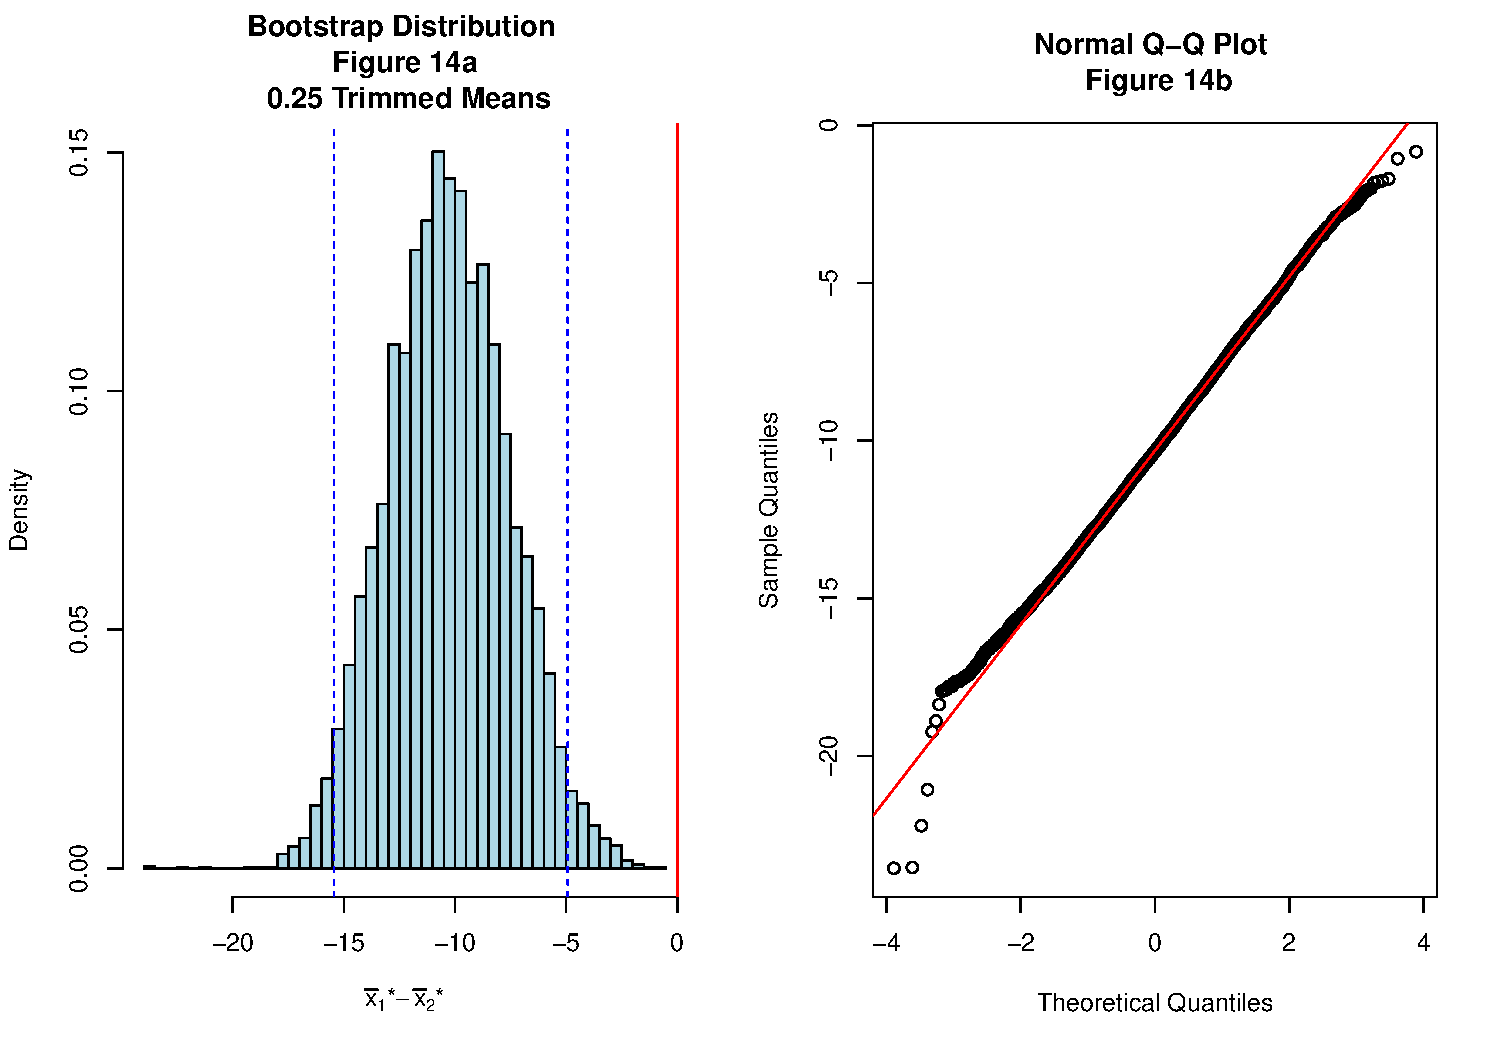
\includegraphics[width=0.6\linewidth,height=0.4\textheight]{Week10_Lect_files/figure-beamer/unnamed-chunk-40-1} \end{center}

\begin{Shaded}
\begin{Highlighting}[]
\FunctionTok{c}\NormalTok{(}\FunctionTok{mean}\NormalTok{(diffmeans), }\FunctionTok{sd}\NormalTok{(diffmeans))}
\end{Highlighting}
\end{Shaded}

\begin{verbatim}
[1] -8.076052  4.016385
\end{verbatim}

\normalsize
\end{frame}

\begin{frame}{Verizon example}
\protect\hypertarget{verizon-example-8}{}
\begin{itemize}
\item
  The bootstrap distribution for the difference in means is shown in
  Figure a.

  \begin{itemize}
  \tightlist
  \item
    Note the strong skewness in the distribution.
  \item
    The mean of the bootstrap distribution is -8.0760517 with a standard
    error of 4.016385.
  \item
    A \(95\%\) bootstrap percentile confidence interval for the
    difference in means (ILEC-CLEC) is given by (-17.1817594,
    -1.6712775).
  \item
    and so we would say that with \(95\%\) confidence, the repair times
    for ILEC customers are, on average, 1.6712775 to 17.1817594 hours
    shorter than the repair times for CLEC customers.
  \end{itemize}
\end{itemize}
\end{frame}

\begin{frame}{Other Statistics}
\protect\hypertarget{other-statistics}{}
\begin{itemize}
\item
  When bootstrapping, we are not limited to simple statistics like the
  simple mean.

  \begin{itemize}
  \tightlist
  \item
    Once we have drawn a bootstrap sample, we can calculate any
    statistic for that sample.
  \item
    means, medians, trimmed means, correlation coefficients, and so on.
  \item
    For example, instead of the sample mean, we can use more robust
    statistics that are less sensitive to extreme observations.
  \item
    It allows statistical inferences such as confidence intervals to be
    calculated even for statistics for which there are no easy formulas.
  \end{itemize}
\item
  Bootstrapping offers hope of reforming statistical practice:

  \begin{itemize}
  \tightlist
  \item
    away from simple but non-robust estimators like a sample mean or
    least-squares regression, in favor of robust alternatives.
  \end{itemize}
\end{itemize}
\end{frame}

\begin{frame}[fragile]{Verizon example}
\protect\hypertarget{verizon-example-9}{}
\begin{itemize}
\item
  Figure below shows the bootstrap distribution for the difference in
  trimmed means, in this case \(25\%\) trimmed means, also known as the
  mid-mean, the mean of the middle \(50\%\) of observations.
\item
  Compared to the bootstrap difference in ordinary means, this
  distribution has a much smaller spread.
\end{itemize}

\tiny

\begin{Shaded}
\begin{Highlighting}[]
\NormalTok{B }\OtherTok{\textless{}{-}} \DecValTok{10}\SpecialCharTok{\^{}}\DecValTok{4}
\NormalTok{diffmeans}\FloatTok{.25} \OtherTok{\textless{}{-}} \FunctionTok{numeric}\NormalTok{(B)}
\FunctionTok{set.seed}\NormalTok{(}\DecValTok{3}\NormalTok{)}
\ControlFlowTok{for}\NormalTok{ (i }\ControlFlowTok{in} \DecValTok{1}\SpecialCharTok{:}\NormalTok{B)\{}
\NormalTok{  ILEC.sample }\OtherTok{\textless{}{-}} \FunctionTok{sample}\NormalTok{(times.ILEC, }\AttributeTok{size =} \FunctionTok{length}\NormalTok{(times.ILEC), }\AttributeTok{replace =} \ConstantTok{TRUE}\NormalTok{)}
\NormalTok{  CLEC.sample }\OtherTok{\textless{}{-}} \FunctionTok{sample}\NormalTok{(times.CLEC, }\AttributeTok{size =} \FunctionTok{length}\NormalTok{(times.CLEC), }\AttributeTok{replace =} \ConstantTok{TRUE}\NormalTok{)}
\NormalTok{  diffmeans}\FloatTok{.25}\NormalTok{[i] }\OtherTok{\textless{}{-}} \FunctionTok{mean}\NormalTok{(ILEC.sample, }\AttributeTok{trim =}\NormalTok{ .}\DecValTok{25}\NormalTok{) }\SpecialCharTok{{-}} \FunctionTok{mean}\NormalTok{(CLEC.sample, }\AttributeTok{trim =}\NormalTok{ .}\DecValTok{25}\NormalTok{)}
\NormalTok{\}}
\NormalTok{CIdiff}\FloatTok{.25} \OtherTok{\textless{}{-}} \FunctionTok{quantile}\NormalTok{(diffmeans}\FloatTok{.25}\NormalTok{, }\AttributeTok{prob =} \FunctionTok{c}\NormalTok{(}\FloatTok{0.025}\NormalTok{, }\FloatTok{0.975}\NormalTok{))}
\NormalTok{CIdiff}\FloatTok{.25}
\end{Highlighting}
\end{Shaded}

\begin{verbatim}
      2.5%      97.5% 
-15.444192  -4.930067 
\end{verbatim}

\normalsize
\end{frame}

\begin{frame}[fragile]{Verizon example}
\protect\hypertarget{verizon-example-10}{}
\tiny

\begin{Shaded}
\begin{Highlighting}[]
\FunctionTok{par}\NormalTok{(}\AttributeTok{mfrow=}\FunctionTok{c}\NormalTok{(}\DecValTok{1}\NormalTok{, }\DecValTok{2}\NormalTok{))}
\FunctionTok{hist}\NormalTok{(diffmeans}\FloatTok{.25}\NormalTok{, }\AttributeTok{breaks =} \StringTok{"Scott"}\NormalTok{, }\AttributeTok{col =} \StringTok{"lightblue"}\NormalTok{, }
     \AttributeTok{main =} \StringTok{"Bootstrap Distribution }\SpecialCharTok{\textbackslash{}n}\StringTok{ Figure 14a }\SpecialCharTok{\textbackslash{}n}\StringTok{ 0.25 Trimmed Means"}\NormalTok{, }
     \AttributeTok{freq=} \ConstantTok{FALSE}\NormalTok{, }\AttributeTok{xlab =} \FunctionTok{substitute}\NormalTok{(}\FunctionTok{paste}\NormalTok{(}\FunctionTok{bar}\NormalTok{(x)[}\DecValTok{1}\NormalTok{],}\StringTok{"*"}\NormalTok{, }\SpecialCharTok{{-}} \FunctionTok{bar}\NormalTok{(x)[}\DecValTok{2}\NormalTok{],}\StringTok{"*"}\NormalTok{)))}
\FunctionTok{abline}\NormalTok{(}\AttributeTok{v =} \FunctionTok{c}\NormalTok{(CIdiff}\FloatTok{.25}\NormalTok{, }\DecValTok{0}\NormalTok{), }\AttributeTok{col =} \FunctionTok{c}\NormalTok{(}\StringTok{"blue"}\NormalTok{, }\StringTok{"blue"}\NormalTok{, }\StringTok{"red"}\NormalTok{), }
       \AttributeTok{lty =} \FunctionTok{c}\NormalTok{(}\StringTok{"dashed"}\NormalTok{, }\StringTok{"dashed"}\NormalTok{, }\StringTok{"solid"}\NormalTok{))}
\FunctionTok{qqnorm}\NormalTok{(diffmeans}\FloatTok{.25}\NormalTok{, }\AttributeTok{main =} \StringTok{"Normal Q{-}Q Plot }\SpecialCharTok{\textbackslash{}n}\StringTok{ Figure 14b"}\NormalTok{)}
\FunctionTok{qqline}\NormalTok{(diffmeans}\FloatTok{.25}\NormalTok{, }\AttributeTok{col =} \StringTok{"red"}\NormalTok{)}
\end{Highlighting}
\end{Shaded}

\begin{center}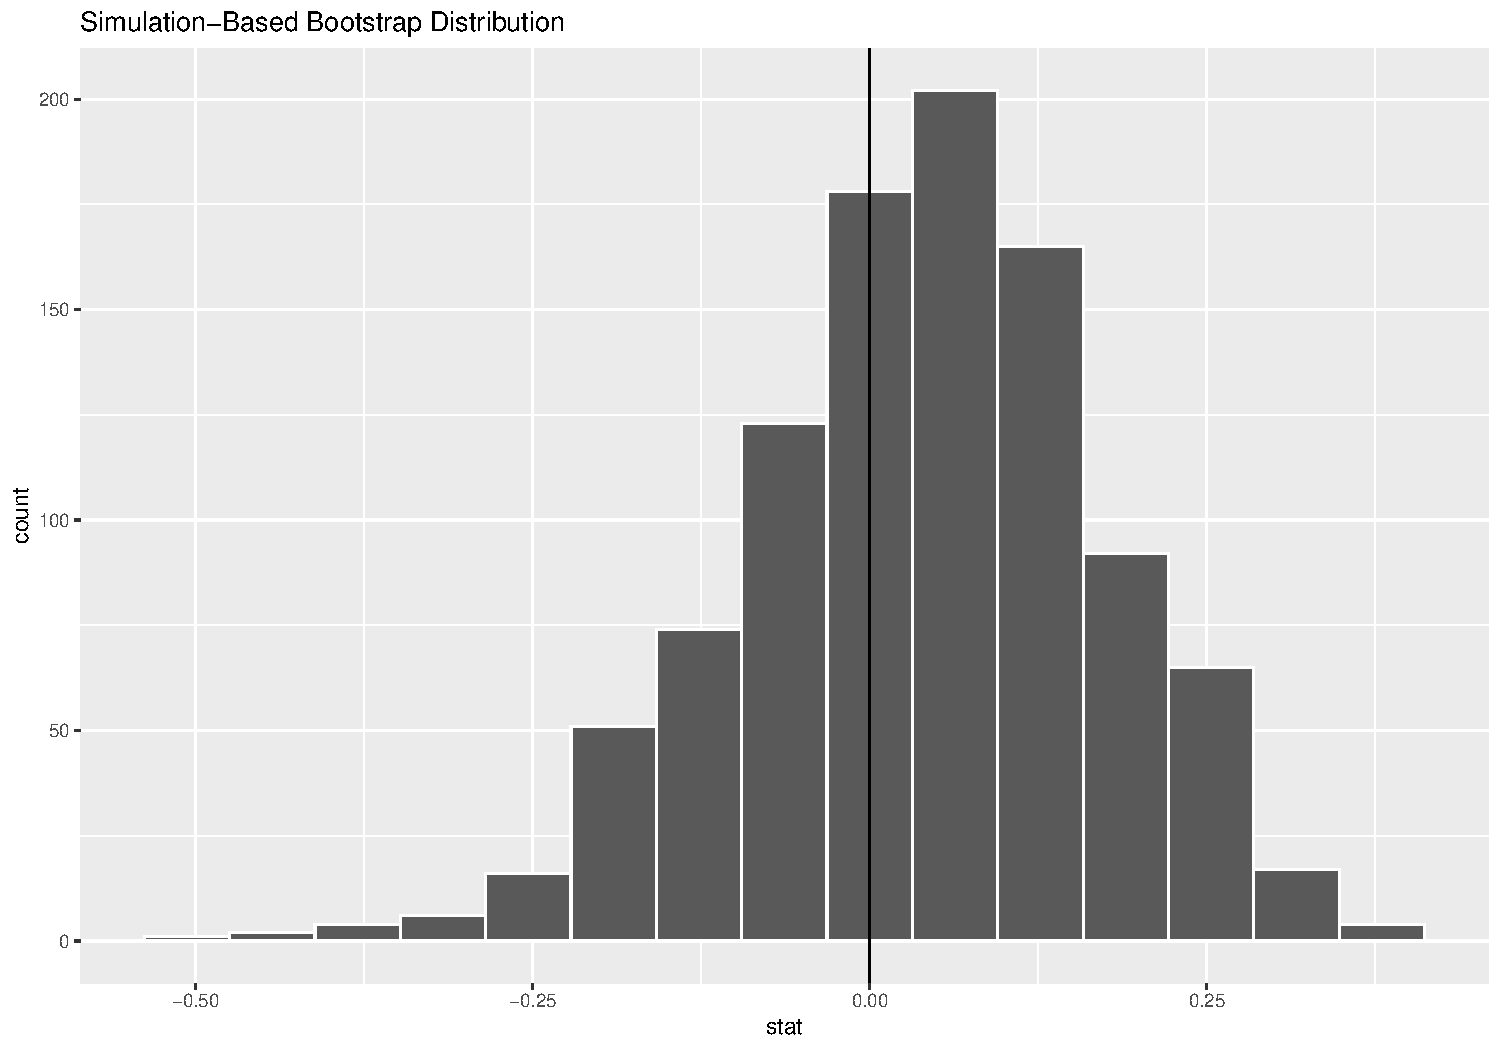
\includegraphics[width=0.6\linewidth,height=0.4\textheight]{Week10_Lect_files/figure-beamer/unnamed-chunk-42-1} \end{center}

\begin{Shaded}
\begin{Highlighting}[]
\FunctionTok{sd}\NormalTok{(diffmeans}\FloatTok{.25}\NormalTok{)}
\end{Highlighting}
\end{Shaded}

\begin{verbatim}
[1] 2.718305
\end{verbatim}

\normalsize
\end{frame}

\begin{frame}[fragile]{Mythbusters example}
\protect\hypertarget{mythbusters-example}{}
\begin{tcolorbox}
Fifty adult participants who thought they were being considered for an appearance on the show were interviewed by a show recruiter. In the interview, the recruiter either yawned or did not. Participants then sat by themselves in a large van and were asked to wait. While in the van, the Mythbusters team watched the participants using a hidden camera to see if they yawned. 
\end{tcolorbox}

\begin{itemize}
\item
  The data frame containing the results of their experiment is available
  in the \texttt{mythbusters\_yawn} data frame included in the
  \texttt{moderndive} package:

  \begin{itemize}
  \tightlist
  \item
    the ``control'' group participants who were not exposed to yawning.
  \item
    the ``seed'' group participants who were exposed to yawning.
  \end{itemize}
\end{itemize}
\end{frame}

\begin{frame}[fragile]{Mythbusters example}
\protect\hypertarget{mythbusters-example-1}{}
\small

\begin{Shaded}
\begin{Highlighting}[]
\FunctionTok{library}\NormalTok{(moderndive)}
\FunctionTok{library}\NormalTok{(tidyverse)}
\FunctionTok{library}\NormalTok{(infer)}
\NormalTok{mythbusters\_yawn }\SpecialCharTok{\%\textgreater{}\%} 
  \FunctionTok{group\_by}\NormalTok{(group, yawn) }\SpecialCharTok{\%\textgreater{}\%} 
  \FunctionTok{summarize}\NormalTok{(}\AttributeTok{count =} \FunctionTok{n}\NormalTok{())}
\end{Highlighting}
\end{Shaded}

\begin{verbatim}
# A tibble: 4 x 3
# Groups:   group [2]
  group   yawn  count
  <chr>   <chr> <int>
1 control no       12
2 control yes       4
3 seed    no       24
4 seed    yes      10
\end{verbatim}

\normalsize
\end{frame}

\begin{frame}[fragile]{Mythbusters example}
\protect\hypertarget{mythbusters-example-2}{}
Here, we are interested in \(p_{seed}-p_{control}\). Let's use
\texttt{infer} pipeline to obtain the bootstrap distribution.

\tiny

\begin{Shaded}
\begin{Highlighting}[]
\FunctionTok{set.seed}\NormalTok{(}\DecValTok{10}\NormalTok{)}
\NormalTok{bootstrap\_distribution\_yawning }\OtherTok{\textless{}{-}}\NormalTok{ mythbusters\_yawn }\SpecialCharTok{\%\textgreater{}\%} 
  \FunctionTok{specify}\NormalTok{(}\AttributeTok{formula =}\NormalTok{ yawn }\SpecialCharTok{\textasciitilde{}}\NormalTok{ group, }\AttributeTok{success =} \StringTok{"yes"}\NormalTok{) }\SpecialCharTok{\%\textgreater{}\%} 
  \FunctionTok{generate}\NormalTok{(}\AttributeTok{reps =} \DecValTok{1000}\NormalTok{, }\AttributeTok{type =} \StringTok{"bootstrap"}\NormalTok{) }\SpecialCharTok{\%\textgreater{}\%} 
  \FunctionTok{calculate}\NormalTok{(}\AttributeTok{stat =} \StringTok{"diff in props"}\NormalTok{, }\AttributeTok{order =} \FunctionTok{c}\NormalTok{(}\StringTok{"seed"}\NormalTok{, }\StringTok{"control"}\NormalTok{))}
\FunctionTok{visualize}\NormalTok{(bootstrap\_distribution\_yawning) }\SpecialCharTok{+}
  \FunctionTok{geom\_vline}\NormalTok{(}\AttributeTok{xintercept =} \DecValTok{0}\NormalTok{)}
\end{Highlighting}
\end{Shaded}

\begin{center}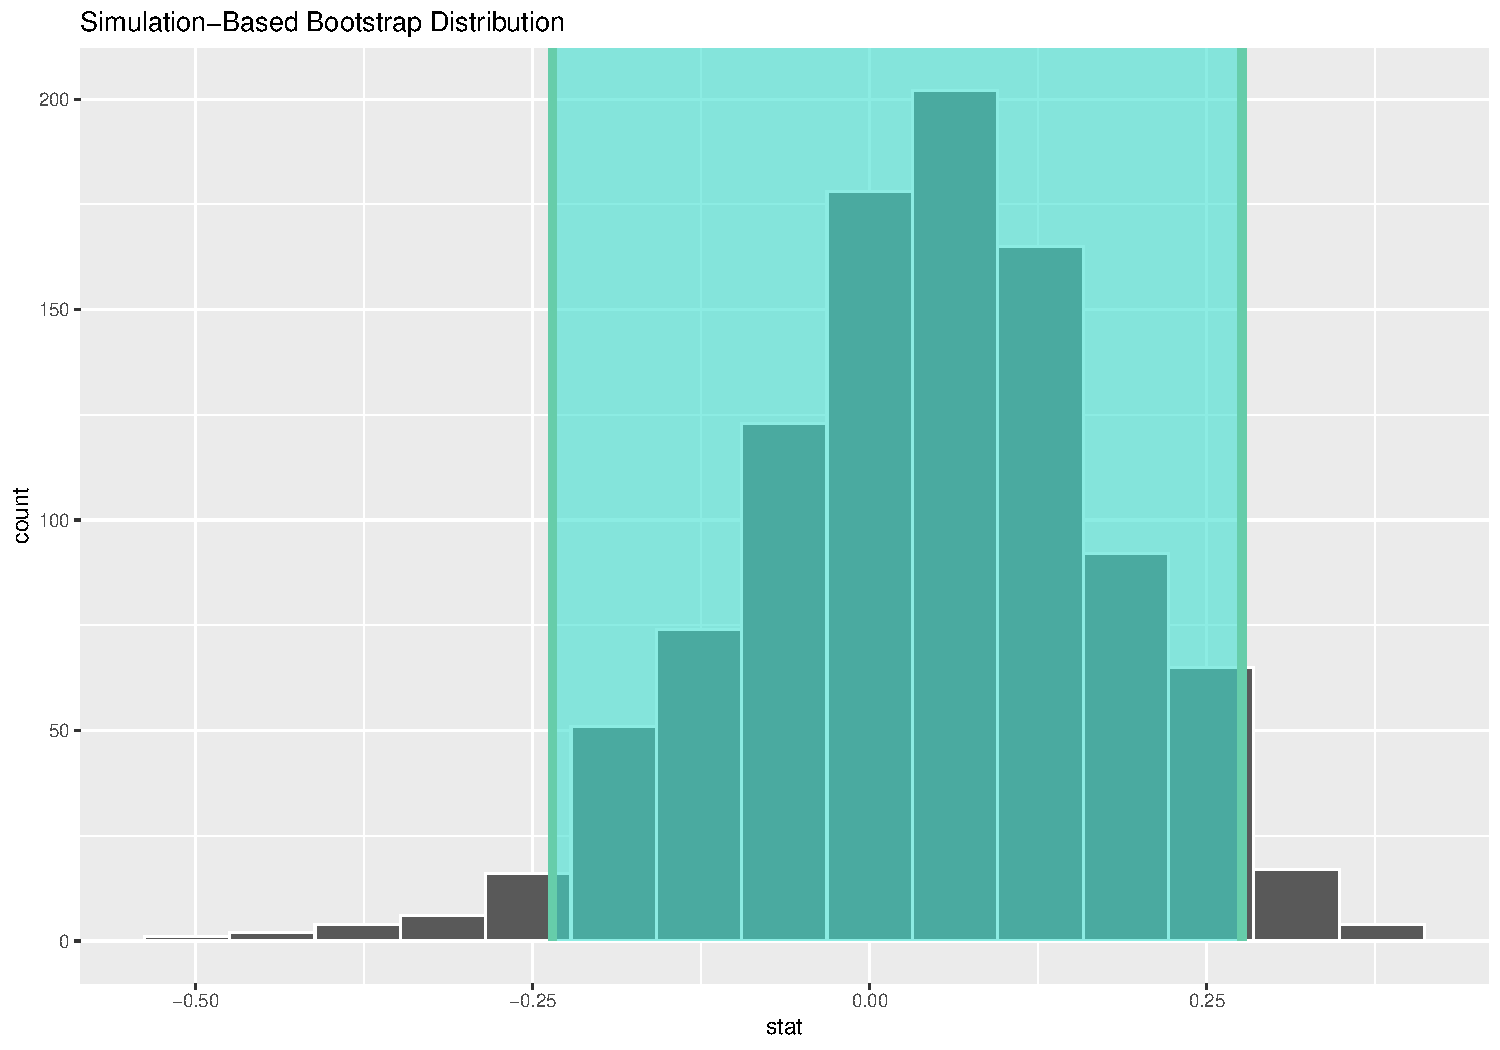
\includegraphics[width=0.6\linewidth,height=0.4\textheight]{Week10_Lect_files/figure-beamer/unnamed-chunk-44-1} \end{center}
\normalsize
\end{frame}

\begin{frame}[fragile]{Mythbusters example}
\protect\hypertarget{mythbusters-example-3}{}
Compute a \(95\%\) confidence interval for \(p_{seed}-p_{control}\)
using the percentile method.

\tiny

\begin{Shaded}
\begin{Highlighting}[]
\NormalTok{percentile\_ci}\OtherTok{\textless{}{-}}\NormalTok{bootstrap\_distribution\_yawning }\SpecialCharTok{\%\textgreater{}\%} 
  \FunctionTok{get\_confidence\_interval}\NormalTok{(}\AttributeTok{type =} \StringTok{"percentile"}\NormalTok{, }\AttributeTok{level =} \FloatTok{0.95}\NormalTok{)}
\NormalTok{percentile\_ci}
\end{Highlighting}
\end{Shaded}

\begin{verbatim}
# A tibble: 1 x 2
  lower_ci upper_ci
     <dbl>    <dbl>
1   -0.235    0.276
\end{verbatim}

\begin{Shaded}
\begin{Highlighting}[]
\NormalTok{obs\_diff\_in\_props }\OtherTok{\textless{}{-}}\NormalTok{ mythbusters\_yawn }\SpecialCharTok{\%\textgreater{}\%} 
  \FunctionTok{specify}\NormalTok{(}\AttributeTok{formula =}\NormalTok{ yawn }\SpecialCharTok{\textasciitilde{}}\NormalTok{ group, }\AttributeTok{success =} \StringTok{"yes"}\NormalTok{) }\SpecialCharTok{\%\textgreater{}\%} 
  \FunctionTok{calculate}\NormalTok{(}\AttributeTok{stat =} \StringTok{"diff in props"}\NormalTok{, }\AttributeTok{order =} \FunctionTok{c}\NormalTok{(}\StringTok{"seed"}\NormalTok{, }\StringTok{"control"}\NormalTok{))}
\NormalTok{obs\_diff\_in\_props}
\end{Highlighting}
\end{Shaded}

\begin{verbatim}
Response: yawn (factor)
Explanatory: group (factor)
# A tibble: 1 x 1
    stat
   <dbl>
1 0.0441
\end{verbatim}

\begin{Shaded}
\begin{Highlighting}[]
\NormalTok{myth\_ci\_se }\OtherTok{\textless{}{-}}\NormalTok{ bootstrap\_distribution\_yawning }\SpecialCharTok{\%\textgreater{}\%} 
  \FunctionTok{get\_confidence\_interval}\NormalTok{(}\AttributeTok{type =} \StringTok{"se"}\NormalTok{, }\AttributeTok{point\_estimate =}\NormalTok{ obs\_diff\_in\_props,}\AttributeTok{level =} \FloatTok{0.95}\NormalTok{)}
\NormalTok{myth\_ci\_se}
\end{Highlighting}
\end{Shaded}

\begin{verbatim}
# A tibble: 1 x 2
  lower_ci upper_ci
     <dbl>    <dbl>
1   -0.217    0.305
\end{verbatim}

\normalsize
\end{frame}

\begin{frame}[fragile]{Mythbusters example}
\protect\hypertarget{mythbusters-example-4}{}
Compute a \(95\%\) confidence interval for \(p_{seed}-p_{control}\)
using the standard error method.

\normalsize

\begin{Shaded}
\begin{Highlighting}[]
\NormalTok{myth\_ci\_se }\OtherTok{\textless{}{-}}\NormalTok{ bootstrap\_distribution\_yawning }\SpecialCharTok{\%\textgreater{}\%} 
  \FunctionTok{get\_confidence\_interval}\NormalTok{(}\AttributeTok{type =} \StringTok{"se"}\NormalTok{, }
                          \AttributeTok{point\_estimate =}\NormalTok{ obs\_diff\_in\_props,}
                          \AttributeTok{level =} \FloatTok{0.95}\NormalTok{)}
\NormalTok{myth\_ci\_se}
\end{Highlighting}
\end{Shaded}

\begin{verbatim}
# A tibble: 1 x 2
  lower_ci upper_ci
     <dbl>    <dbl>
1   -0.217    0.305
\end{verbatim}

\normalsize
\end{frame}

\begin{frame}[fragile]{Mythbusters example}
\protect\hypertarget{mythbusters-example-5}{}
\tiny

\begin{Shaded}
\begin{Highlighting}[]
\FunctionTok{visualize}\NormalTok{(bootstrap\_distribution\_yawning) }\SpecialCharTok{+}
\FunctionTok{shade\_confidence\_interval}\NormalTok{(}\AttributeTok{endpoints =}\NormalTok{ percentile\_ci)}
\end{Highlighting}
\end{Shaded}

\begin{center}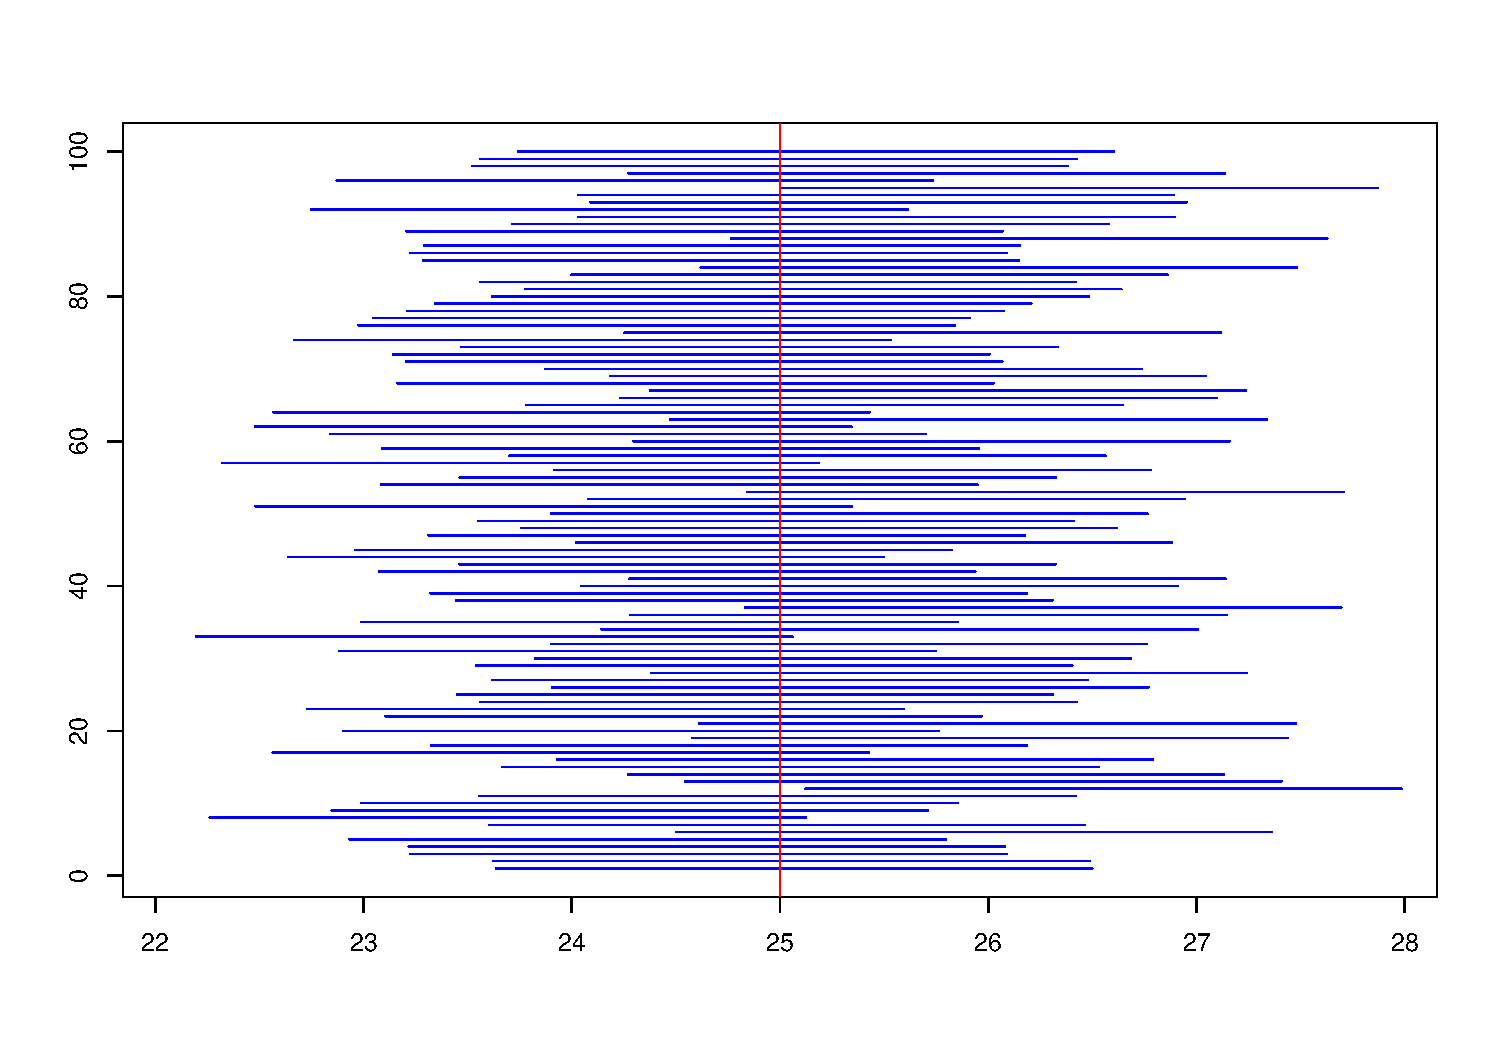
\includegraphics[width=0.6\linewidth,height=0.4\textheight]{Week10_Lect_files/figure-beamer/unnamed-chunk-47-1} \end{center}
\normalsize

\begin{itemize}
\item
  We're \(95\%\) ``confident'' that the true difference in proportions
  \(p_{seed}-p_{control}\) is between (-0.235, 0.276).

  \begin{itemize}
  \tightlist
  \item
    Since the interval includes 0, we cannot conclusively say if either
    proportion is larger.
  \item
    This would suggest that there is no associated effect of being
    exposed to a yawning recruiter on whether you yawn yourself.
  \end{itemize}
\end{itemize}
\end{frame}

\hypertarget{theory-based-confidence-intervals}{%
\section{Theory-based confidence
intervals}\label{theory-based-confidence-intervals}}

\begin{frame}{Theory-based confidence intervals}
\protect\hypertarget{theory-based-confidence-intervals-1}{}
\begin{itemize}
\item
  So far, we've constructed confidence intervals using two methods:

  \begin{itemize}
  \tightlist
  \item
    the percentile method and the standard error method.
  \end{itemize}
\item
  We can only use the standard-error method if the bootstrap
  distribution is bell-shaped (i.e., normally distributed).
\item
  If the sampling distribution is normally shaped, there is another
  method for constructing confidence intervals that does not involve
  using your computer.

  \begin{itemize}
  \tightlist
  \item
    You can use a theory-based method involving mathematical formulas!
  \end{itemize}
\end{itemize}
\end{frame}

\begin{frame}{Confidence intervals for a Mean, \(\sigma\) known}
\protect\hypertarget{confidence-intervals-for-a-mean-sigma-known}{}
\begin{tcolorbox}
The Centers for Disease Control maintains growth charts for infants and children (http://cdc.gov/growthcharts/zscore.html). For 13-year-old girls, the mean weight is 101 pounds with a standard deviation of 24.6 pounds. We assume the weights are normally distributed. The public health officials in Sodor are interested in the weights of the teens in their town: they suspect that the mean weight of their girls might be different from the mean weight in the growth chart but are willing to assume that the variation is the same. If they survey a random sample of 150 thirteen-year-old girls and find their mean weight – an estimate of the population mean weight – is 95 pounds, how accurate will this estimate be?
\end{tcolorbox}
\end{frame}

\begin{frame}{Confidence intervals for a Mean, \(\sigma\) known}
\protect\hypertarget{confidence-intervals-for-a-mean-sigma-known-1}{}
We assume the 150 sample values are from a normal distribution,
\(N(\mu, 24.6)\).

\begin{itemize}
\item
  Then the sampling distribution of mean weights is
  \[N\left(\mu,\frac{24.6}{\sqrt{150}}\right)\]
\item
  Let \(\bar{X}\) denote the mean of the 150 weights, so standardizing
  gives \[Z=\frac{\bar{X}-\mu}{\frac{24.6}{\sqrt{150}}}\sim N(0,1)\]
\end{itemize}
\end{frame}

\begin{frame}{Confidence intervals for a Mean, \(\sigma\) known}
\protect\hypertarget{confidence-intervals-for-a-mean-sigma-known-2}{}
\begin{itemize}
\tightlist
\item
  For a standard normal random variable \(Z\), we have:
  \[1-\alpha=P(z_{\alpha/2}<Z<z_{1-\alpha/2})\] Then:
  \[0.95=P\left(z_{0.025}<\frac{\bar{X}-\mu}{\frac{24.6}{\sqrt{150}}}<z_{0.975}\right)\]
  \[0.95=P\left(\bar{X}+z_{0.025}\times\frac{24.6}{\sqrt{150}}<\mu<\bar{X}+z_{0.975}\times\frac{24.6}{\sqrt{150}}\right)\]
  \[0.95=P\left(\bar{X}-1.96\times\frac{24.6}{\sqrt{150}}<\mu<\bar{X}+1.96\times\frac{24.6}{\sqrt{150}}\right)\]
  \[0.95=P(\bar{X}-3.937<\mu<\bar{X}+3.937)\]
\end{itemize}

This means that, the random interval \(\bar{X}-3.937<\mu<\bar{X}+3.937\)
has a probability of 0.95 of containing the mean \(\mu\).
\end{frame}

\begin{frame}{Confidence intervals for a Mean, \(\sigma\) known}
\protect\hypertarget{confidence-intervals-for-a-mean-sigma-known-3}{}
\begin{itemize}
\tightlist
\item
  Now, the random variable \(\bar{X}\) is replaced by the (observed)
  sample mean weight of \(\bar{x}=95\), we obtain: \[\begin{array}{ll}
  (\bar{X}-3.937<\mu<\bar{X}+3.937)=(95-3.937<\mu<95+3.937)\\
  =(91.1, 98.9)\end{array}\]
\end{itemize}

Which is no longer a random interval.

\begin{itemize}
\tightlist
\item
  We interpret this interval by stating that we are \(95\%\) confident
  that the population mean weight of 13-year-old girls in Sodor is
  between 91.9 and 98.9 pounds.
\end{itemize}
\end{frame}

\begin{frame}{Confidence intervals for a Mean, \(\sigma\) known}
\protect\hypertarget{confidence-intervals-for-a-mean-sigma-known-4}{}
More generally, for a sample of size \(n\) drawn from a normal
distribution with unknown \(\mu\), and known \(\sigma\), a
\((1-\alpha)\times 100\%\) confidence interval for the mean of \(\mu\)
is:

\[CI_{1-\alpha}(\mu)=\left(\bar{X}-z_{1-\alpha/2}\frac{\sigma}{\sqrt{n}},\bar{X}+z_{1-\alpha/2}\frac{\sigma}{\sqrt{n}}\right)\]

If we draw thousands of random samples from a normal distribution with
parameters \(\mu\), \(\sigma\) and compute the \(95\%\) confidence
interval for each sample, then about \(95\%\) of the intervals would
contain \(\mu\).
\end{frame}

\begin{frame}[fragile]{Confidence intervals for a Mean, \(\sigma\)
known}
\protect\hypertarget{confidence-intervals-for-a-mean-sigma-known-5}{}
\normalsize

\begin{Shaded}
\begin{Highlighting}[]
\FunctionTok{set.seed}\NormalTok{(}\DecValTok{13}\NormalTok{)}
\NormalTok{counter }\OtherTok{\textless{}{-}} \DecValTok{0} \CommentTok{\# set counter to 0}
\NormalTok{mu }\OtherTok{\textless{}{-}} \DecValTok{25}
\NormalTok{sigma }\OtherTok{\textless{}{-}} \DecValTok{4}
\NormalTok{n }\OtherTok{\textless{}{-}} \DecValTok{30}
\NormalTok{sims }\OtherTok{\textless{}{-}} \DecValTok{10}\SpecialCharTok{\^{}}\DecValTok{4}
\FunctionTok{plot}\NormalTok{(}\AttributeTok{x =} \FunctionTok{c}\NormalTok{(mu }\SpecialCharTok{{-}} \DecValTok{4}\SpecialCharTok{*}\NormalTok{sigma}\SpecialCharTok{/}\FunctionTok{sqrt}\NormalTok{(n), mu }\SpecialCharTok{+} \DecValTok{4}\SpecialCharTok{*}\NormalTok{sigma}\SpecialCharTok{/}\FunctionTok{sqrt}\NormalTok{(n)), }
     \AttributeTok{y =} \FunctionTok{c}\NormalTok{(}\DecValTok{1}\NormalTok{, }\DecValTok{100}\NormalTok{), }\AttributeTok{type =} \StringTok{"n"}\NormalTok{, }\AttributeTok{xlab =} \StringTok{""}\NormalTok{, }\AttributeTok{ylab =} \StringTok{""}\NormalTok{)}
\ControlFlowTok{for}\NormalTok{ (i }\ControlFlowTok{in} \DecValTok{1}\SpecialCharTok{:}\NormalTok{sims)\{}
\NormalTok{ x }\OtherTok{\textless{}{-}} \FunctionTok{rnorm}\NormalTok{(n, mu, sigma)}
\NormalTok{ L }\OtherTok{\textless{}{-}} \FunctionTok{mean}\NormalTok{(x) }\SpecialCharTok{{-}} \FunctionTok{qnorm}\NormalTok{(}\FloatTok{0.975}\NormalTok{)}\SpecialCharTok{*}\NormalTok{sigma}\SpecialCharTok{/}\FunctionTok{sqrt}\NormalTok{(n)}
\NormalTok{ U }\OtherTok{\textless{}{-}} \FunctionTok{mean}\NormalTok{(x) }\SpecialCharTok{{-}} \FunctionTok{qnorm}\NormalTok{(}\FloatTok{0.025}\NormalTok{)}\SpecialCharTok{*}\NormalTok{sigma}\SpecialCharTok{/}\FunctionTok{sqrt}\NormalTok{(n)}
 \ControlFlowTok{if}\NormalTok{(L }\SpecialCharTok{\textless{}}\NormalTok{ mu }\SpecialCharTok{\&\&}\NormalTok{ mu }\SpecialCharTok{\textless{}}\NormalTok{ U)\{counter }\OtherTok{\textless{}{-}}\NormalTok{ counter }\SpecialCharTok{+} \DecValTok{1}\NormalTok{\}}
 \ControlFlowTok{if}\NormalTok{(i }\SpecialCharTok{\textless{}=} \DecValTok{100}\NormalTok{)\{}
 \FunctionTok{segments}\NormalTok{(L, i, U, i, }\AttributeTok{col =} \StringTok{"blue"}\NormalTok{)}
\NormalTok{ \}}
\NormalTok{\}}
\FunctionTok{abline}\NormalTok{(}\AttributeTok{v =}\NormalTok{ mu, }\AttributeTok{col =} \StringTok{"red"}\NormalTok{)}
\end{Highlighting}
\end{Shaded}

\normalsize
\end{frame}

\begin{frame}[fragile]{Confidence intervals for a Mean, \(\sigma\)
known}
\protect\hypertarget{confidence-intervals-for-a-mean-sigma-known-6}{}
\begin{center}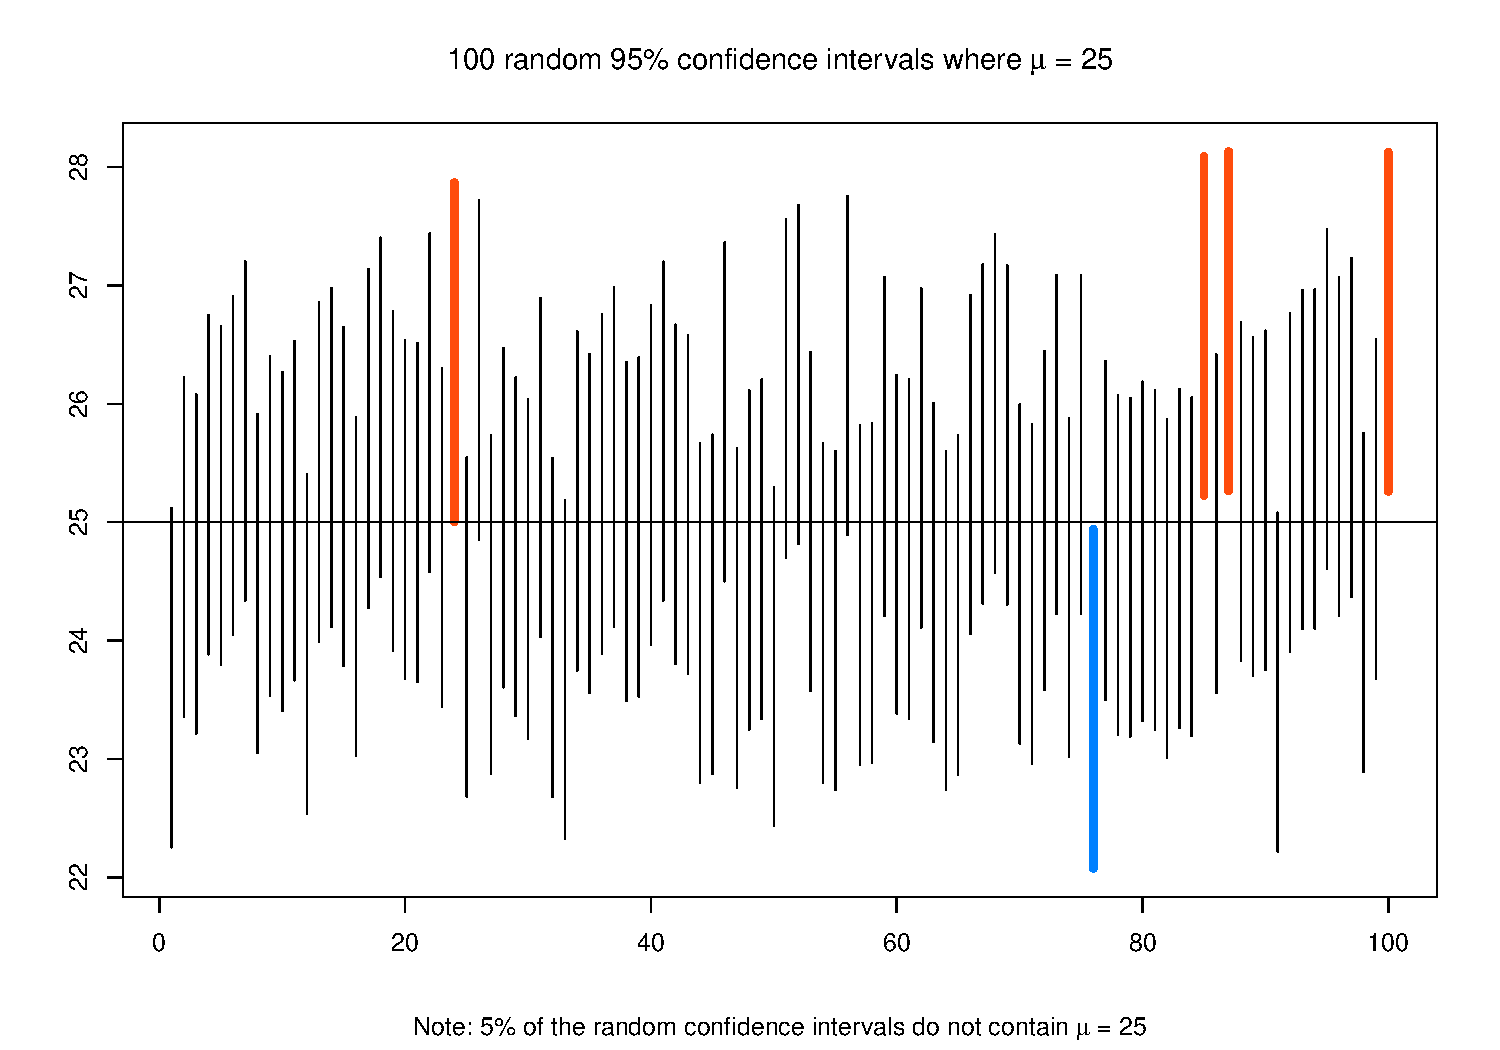
\includegraphics[width=0.6\linewidth,height=0.7\textheight]{Week10_Lect_files/figure-beamer/unnamed-chunk-49-1} \end{center}
\normalsize

\tiny

\begin{Shaded}
\begin{Highlighting}[]
\NormalTok{ACL }\OtherTok{\textless{}{-}}\NormalTok{ counter}\SpecialCharTok{/}\NormalTok{sims}\SpecialCharTok{*}\DecValTok{100}
\NormalTok{ACL}
\end{Highlighting}
\end{Shaded}

\begin{verbatim}
[1] 95.08
\end{verbatim}

\normalsize
\end{frame}

\begin{frame}[fragile]{Confidence intervals for a Mean, \(\sigma\)
known}
\protect\hypertarget{confidence-intervals-for-a-mean-sigma-known-7}{}
\normalsize

\begin{Shaded}
\begin{Highlighting}[]
\FunctionTok{library}\NormalTok{(PASWR2)}
\FunctionTok{set.seed}\NormalTok{(}\DecValTok{11}\NormalTok{)}
\FunctionTok{cisim}\NormalTok{(}\AttributeTok{samples =} \DecValTok{100}\NormalTok{, }\AttributeTok{n =} \DecValTok{30}\NormalTok{, }\AttributeTok{parameter =} \DecValTok{25}\NormalTok{, }\AttributeTok{sigma =} \DecValTok{4}\NormalTok{, }
      \AttributeTok{type =} \StringTok{"Mean"}\NormalTok{)}
\end{Highlighting}
\end{Shaded}

\begin{center}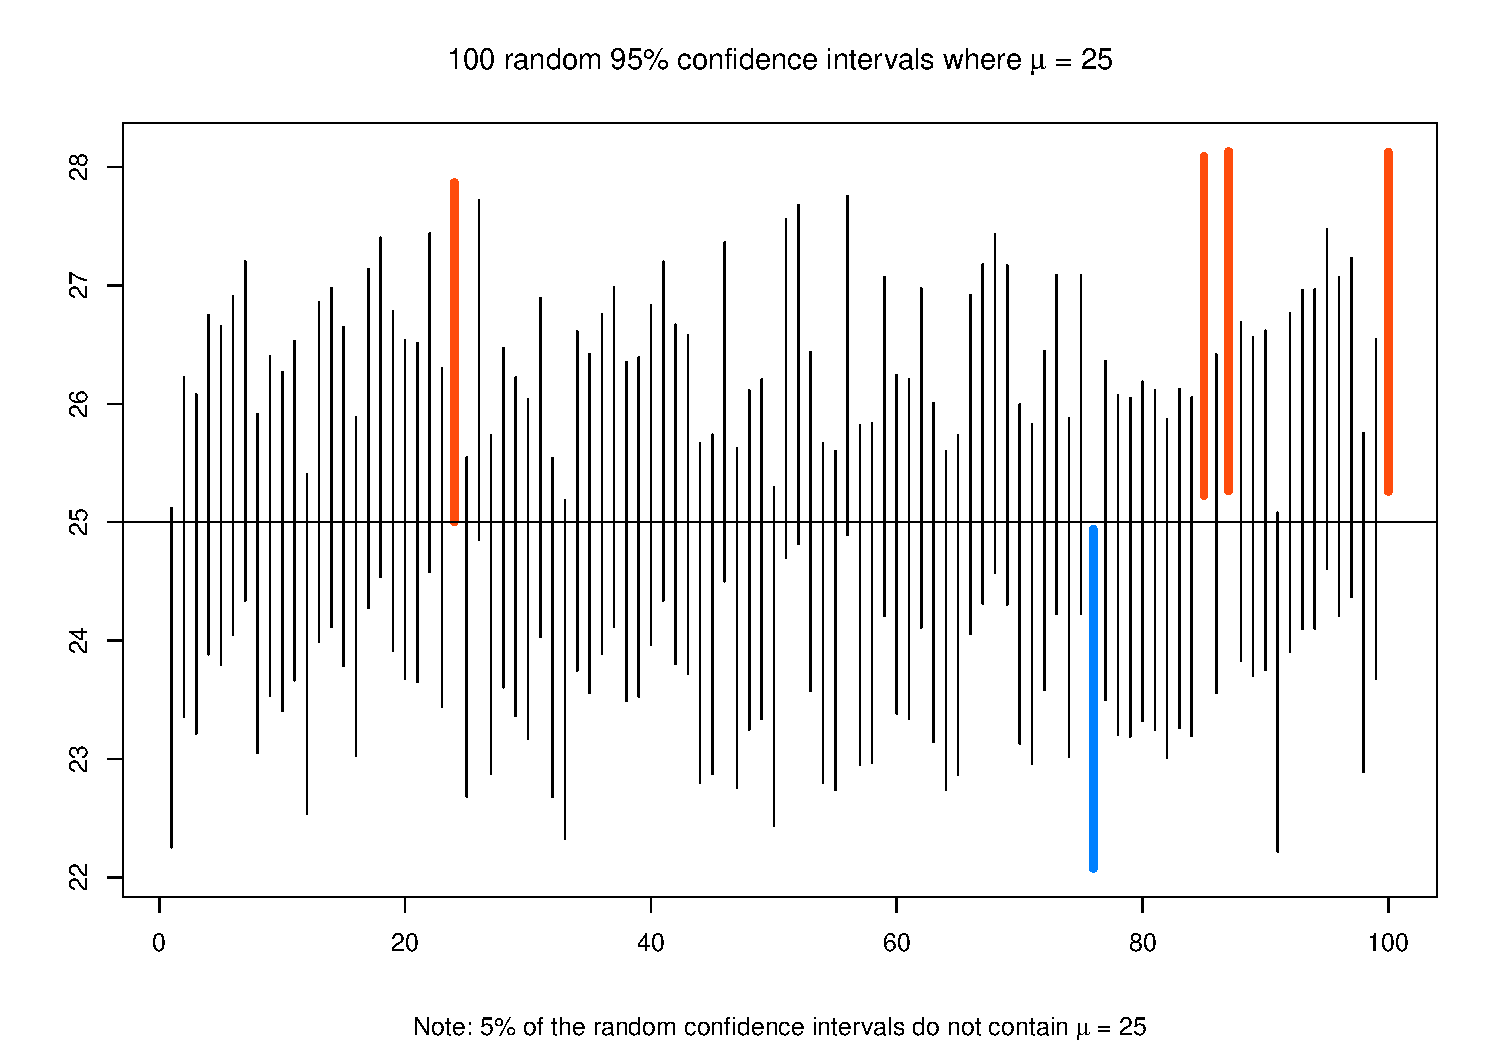
\includegraphics[width=0.6\linewidth,height=0.4\textheight]{Week10_Lect_files/figure-beamer/unnamed-chunk-51-1} \end{center}

\begin{verbatim}

5% of the random confidence intervals do not contain Mu = 25.
\end{verbatim}

\normalsize
\end{frame}

\begin{frame}{Example 2}
\protect\hypertarget{example-2}{}
\begin{tcolorbox}
An engineer test the gas mileage of a random sample of $n=30$ of his company cars ready to be sold. The $95\%$ confidence interval for the mean mileage of all the cars is $(29.5, 33.4)$ miles per gallon. Evaluate the following statements:
\begin{itemize}
\item We are $95\%$ confident that the gas mileage for cars in this company is between 29.5 and 33.4 mpg.

\item $95\%$ of all samples will give an average mileage between 29.5 and 33.4 mpg.

\item There is a $95\%$ chance that the true mean is between 29.5 and 33.4 mpg.
\end{itemize}
\end{tcolorbox}
\end{frame}

\begin{frame}{Example 2}
\protect\hypertarget{example-2-1}{}
\begin{tcolorbox}
Solution: 

\vspace{30mm}

\end{tcolorbox}
\end{frame}

\begin{frame}{Example 3}
\protect\hypertarget{example-3}{}
\begin{tcolorbox}
 Suppose the sample 3.4, 2.9, 2.8, 5.1, 6.3, 3.9 is drawn from the normal distribution with unknown $\mu$ and known $\sigma=2.5$. Find a $90\%$ confidence interval for $\mu$.
\end{tcolorbox}

\begin{tcolorbox}
Solution: 

\vspace{30mm}


\end{tcolorbox}
\end{frame}

\begin{frame}[fragile]{Example 3}
\protect\hypertarget{example-3-1}{}
\small

\begin{Shaded}
\begin{Highlighting}[]
\NormalTok{xs }\OtherTok{\textless{}{-}} \FunctionTok{c}\NormalTok{(}\FloatTok{3.4}\NormalTok{, }\FloatTok{2.9}\NormalTok{, }\FloatTok{2.8}\NormalTok{, }\FloatTok{5.1}\NormalTok{, }\FloatTok{6.3}\NormalTok{, }\FloatTok{3.9}\NormalTok{)}
\NormalTok{n }\OtherTok{\textless{}{-}} \FunctionTok{length}\NormalTok{(xs)}
\NormalTok{SIGMA }\OtherTok{\textless{}{-}} \FloatTok{2.5}
\NormalTok{alpha }\OtherTok{\textless{}{-}} \FloatTok{0.10}
\NormalTok{LL }\OtherTok{\textless{}{-}} \FunctionTok{mean}\NormalTok{(xs) }\SpecialCharTok{{-}} \FunctionTok{qnorm}\NormalTok{(}\DecValTok{1} \SpecialCharTok{{-}}\NormalTok{ alpha}\SpecialCharTok{/}\DecValTok{2}\NormalTok{)}\SpecialCharTok{*}\NormalTok{SIGMA}\SpecialCharTok{/}\FunctionTok{sqrt}\NormalTok{(n)}
\NormalTok{UL }\OtherTok{\textless{}{-}} \FunctionTok{mean}\NormalTok{(xs) }\SpecialCharTok{+} \FunctionTok{qnorm}\NormalTok{(}\DecValTok{1} \SpecialCharTok{{-}}\NormalTok{ alpha}\SpecialCharTok{/}\DecValTok{2}\NormalTok{)}\SpecialCharTok{*}\NormalTok{SIGMA}\SpecialCharTok{/}\FunctionTok{sqrt}\NormalTok{(n)}
\NormalTok{CI }\OtherTok{\textless{}{-}} \FunctionTok{c}\NormalTok{(LL, UL)}
\NormalTok{CI}
\end{Highlighting}
\end{Shaded}

\begin{verbatim}
[1] 2.387895 5.745438
\end{verbatim}

\begin{Shaded}
\begin{Highlighting}[]
\CommentTok{\# or use z.test() from PASWR2}
\FunctionTok{z.test}\NormalTok{(}\AttributeTok{x =}\NormalTok{ xs, }\AttributeTok{sigma.x =}\NormalTok{ SIGMA, }\AttributeTok{conf.level =} \FloatTok{0.90}\NormalTok{)}\SpecialCharTok{$}\NormalTok{conf}
\end{Highlighting}
\end{Shaded}

\begin{verbatim}
[1] 2.387895 5.745438
attr(,"conf.level")
[1] 0.9
\end{verbatim}

\normalsize

\begin{itemize}
\item
  The term \(z_{1-\alpha/2}\times \sigma/\sqrt{n}\) is called the margin
  of error (we abbreviate this as ME).

  \begin{itemize}
  \tightlist
  \item
    The margin of error for a symmetric confidence interval is the
    distance from the estimate to either end.
  \end{itemize}
\end{itemize}
\end{frame}

\begin{frame}{Example 4}
\protect\hypertarget{example-4}{}
\begin{tcolorbox}
Suppose researchers want to estimate the mean weight of girls in Sodor. They assume that the distribution of weights is normal with unknown mean $\mu$, but with known $\sigma=24.6$. How many girls should they sample if they want, with $95\%$ confidence, their margin of error to be at most 5 pounds?
\end{tcolorbox}

\begin{tcolorbox}


\vspace{30mm}

\end{tcolorbox}
\end{frame}

\begin{frame}[fragile]{Example 4}
\protect\hypertarget{example-4-1}{}
\normalsize

\begin{Shaded}
\begin{Highlighting}[]
\NormalTok{n }\OtherTok{\textless{}{-}} \FunctionTok{ceiling}\NormalTok{((}\FunctionTok{qnorm}\NormalTok{(.}\DecValTok{975}\NormalTok{)}\SpecialCharTok{*}\FloatTok{24.6}\SpecialCharTok{/}\DecValTok{5}\NormalTok{)}\SpecialCharTok{\^{}}\DecValTok{2}\NormalTok{)}
\NormalTok{n}
\end{Highlighting}
\end{Shaded}

\begin{verbatim}
[1] 93
\end{verbatim}

\begin{Shaded}
\begin{Highlighting}[]
\CommentTok{\# Using nsize from PASWR2}
\FunctionTok{nsize}\NormalTok{(}\AttributeTok{b =} \DecValTok{5}\NormalTok{, }\AttributeTok{sigma =} \FloatTok{24.6}\NormalTok{, }\AttributeTok{conf.level =} \FloatTok{0.95}\NormalTok{, }\AttributeTok{type =} \StringTok{"mu"}\NormalTok{)}
\end{Highlighting}
\end{Shaded}

\begin{verbatim}

The required sample size (n) to estimate the population 
mean with a 0.95 confidence interval so that the margin 
of error is no more than 5 is 93.
\end{verbatim}

\normalsize

\begin{itemize}
\item
  Note: To make the confidence interval narrower, analysts can either

  \begin{itemize}
  \tightlist
  \item
    increase the sample size \(n\) or
  \item
    decrease the size of the quantile \(z_{1-\alpha/2}\), which amounts
    to decreasing the confidence level.
  \end{itemize}
\end{itemize}
\end{frame}

\begin{frame}{Confidence intervals for a Mean, \(\sigma\) unknown}
\protect\hypertarget{confidence-intervals-for-a-mean-sigma-unknown}{}
In most real-life settings, a data analyst will not know the mean or the
standard deviation of the population of interest.

\begin{itemize}
\item
  How then would we get an interval estimate of the mean \(\mu\)?

  \begin{itemize}
  \tightlist
  \item
    we have used the sample mean \(\bar{X}\) as an estimate of \(\mu\).
  \item
    so it seems natural to consider the sample standard deviation \(S\)
    as an estimate of \(\sigma\).
  \end{itemize}
\item
  However, in deriving the confidence interval for \(\mu\), we used the
  fact that \(\frac{(\bar{X}-\mu)}{\sigma/\sqrt{n}}\) follows a standard
  normal distribution.
\item
  Does changing \(\sigma\) to \(S\), the sample standard deviation,
  change the distribution?

  \begin{itemize}
  \tightlist
  \item
    We will use simulation to investigate the distribution of
    \(\frac{(\bar{X}-\mu)}{\sigma/\sqrt{n}}\) for random samples drawn
    from a \(N(\mu, \sigma)\).
  \end{itemize}
\end{itemize}
\end{frame}

\begin{frame}[fragile]{Confidence intervals for a Mean, \(\sigma\)
unknown}
\protect\hypertarget{confidence-intervals-for-a-mean-sigma-unknown-1}{}
\tiny

\begin{Shaded}
\begin{Highlighting}[]
\FunctionTok{set.seed}\NormalTok{(}\DecValTok{1}\NormalTok{)}
\NormalTok{N }\OtherTok{\textless{}{-}} \DecValTok{10}\SpecialCharTok{\^{}}\DecValTok{4}
\NormalTok{TS }\OtherTok{\textless{}{-}} \FunctionTok{numeric}\NormalTok{(N)}
\NormalTok{n }\OtherTok{\textless{}{-}} \DecValTok{16}
\ControlFlowTok{for}\NormalTok{(i }\ControlFlowTok{in} \DecValTok{1}\SpecialCharTok{:}\NormalTok{N)\{}
\NormalTok{  x }\OtherTok{\textless{}{-}} \FunctionTok{rnorm}\NormalTok{(n, }\DecValTok{25}\NormalTok{, }\DecValTok{7}\NormalTok{)}
\NormalTok{  xbar }\OtherTok{\textless{}{-}} \FunctionTok{mean}\NormalTok{(x)}
\NormalTok{  s }\OtherTok{\textless{}{-}} \FunctionTok{sd}\NormalTok{(x)}
\NormalTok{  TS[i] }\OtherTok{\textless{}{-}}\NormalTok{ (xbar }\SpecialCharTok{{-}} \DecValTok{25}\NormalTok{)}\SpecialCharTok{/}\NormalTok{(s}\SpecialCharTok{/}\FunctionTok{sqrt}\NormalTok{(n))}
\NormalTok{\}}
\FunctionTok{par}\NormalTok{(}\AttributeTok{mfrow=}\FunctionTok{c}\NormalTok{(}\DecValTok{1}\NormalTok{, }\DecValTok{2}\NormalTok{))}
\FunctionTok{hist}\NormalTok{(TS, }\AttributeTok{breaks =} \StringTok{"Scott"}\NormalTok{, }\AttributeTok{freq =} \ConstantTok{FALSE}\NormalTok{, }\AttributeTok{col =} \StringTok{"pink"}\NormalTok{, }\AttributeTok{main =} \StringTok{""}\NormalTok{, }\AttributeTok{xlab =} \FunctionTok{expression}\NormalTok{(t))}
\FunctionTok{qqnorm}\NormalTok{(TS, }\AttributeTok{col =} \FunctionTok{rgb}\NormalTok{(}\DecValTok{1}\NormalTok{, }\DecValTok{0}\NormalTok{, }\DecValTok{0}\NormalTok{, .}\DecValTok{1}\NormalTok{))}
\FunctionTok{abline}\NormalTok{(}\AttributeTok{a =} \DecValTok{0}\NormalTok{, }\AttributeTok{b =} \DecValTok{1}\NormalTok{)}
\end{Highlighting}
\end{Shaded}

\begin{center}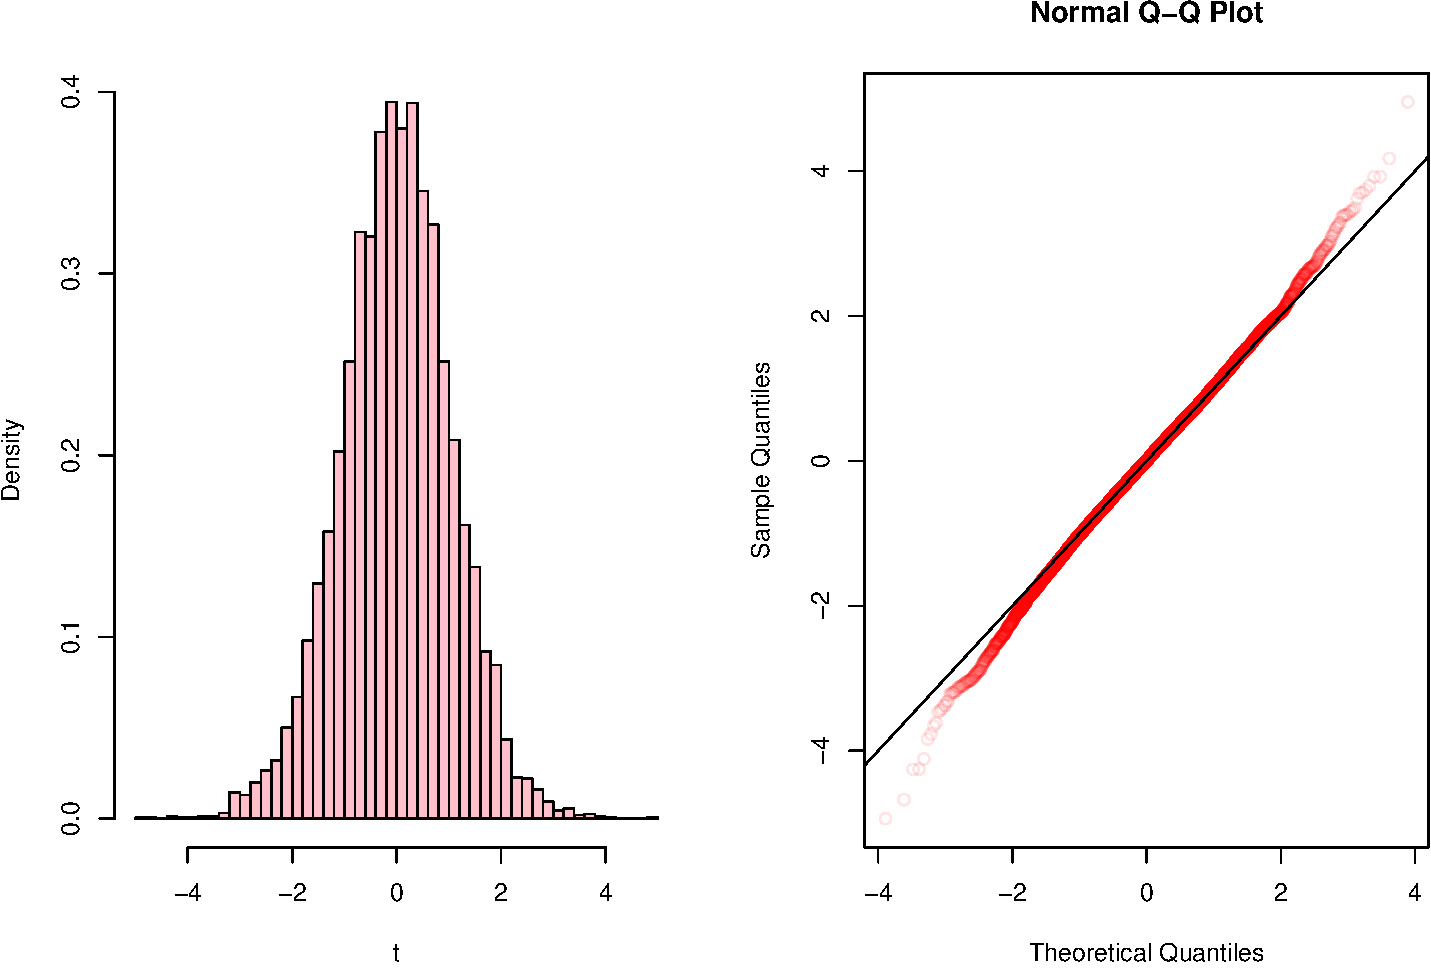
\includegraphics[width=0.6\linewidth,height=0.4\textheight]{Week10_Lect_files/figure-beamer/unnamed-chunk-54-1} \end{center}
\normalsize
\end{frame}

\begin{frame}[fragile]{Confidence intervals for a Mean, \(\sigma\)
unknown}
\protect\hypertarget{confidence-intervals-for-a-mean-sigma-unknown-2}{}
Consider qq plot for \(t_{24}\)

\tiny

\begin{Shaded}
\begin{Highlighting}[]
\CommentTok{\# Consider qq plot for t\_24}
\FunctionTok{ggplot}\NormalTok{(}\AttributeTok{data =} \FunctionTok{data.frame}\NormalTok{(}\AttributeTok{x =}\NormalTok{ TS), }\FunctionTok{aes}\NormalTok{(}\AttributeTok{sample =}\NormalTok{ x)) }\SpecialCharTok{+} 
  \FunctionTok{geom\_qq}\NormalTok{(}\AttributeTok{distribution =}\NormalTok{ stats}\SpecialCharTok{::}\NormalTok{qt, }\AttributeTok{dparams =} \FunctionTok{list}\NormalTok{(}\AttributeTok{df =} \DecValTok{24}\NormalTok{), }\AttributeTok{size =} \FloatTok{0.1}\NormalTok{, }\AttributeTok{color =} \StringTok{"blue"}\NormalTok{) }\SpecialCharTok{+} 
  \FunctionTok{geom\_abline}\NormalTok{(}\AttributeTok{intercept =} \DecValTok{0}\NormalTok{, }\AttributeTok{slope =} \DecValTok{1}\NormalTok{, }\AttributeTok{color =} \StringTok{"pink"}\NormalTok{) }\SpecialCharTok{+} 
  \FunctionTok{theme\_bw}\NormalTok{()}
\end{Highlighting}
\end{Shaded}

\begin{center}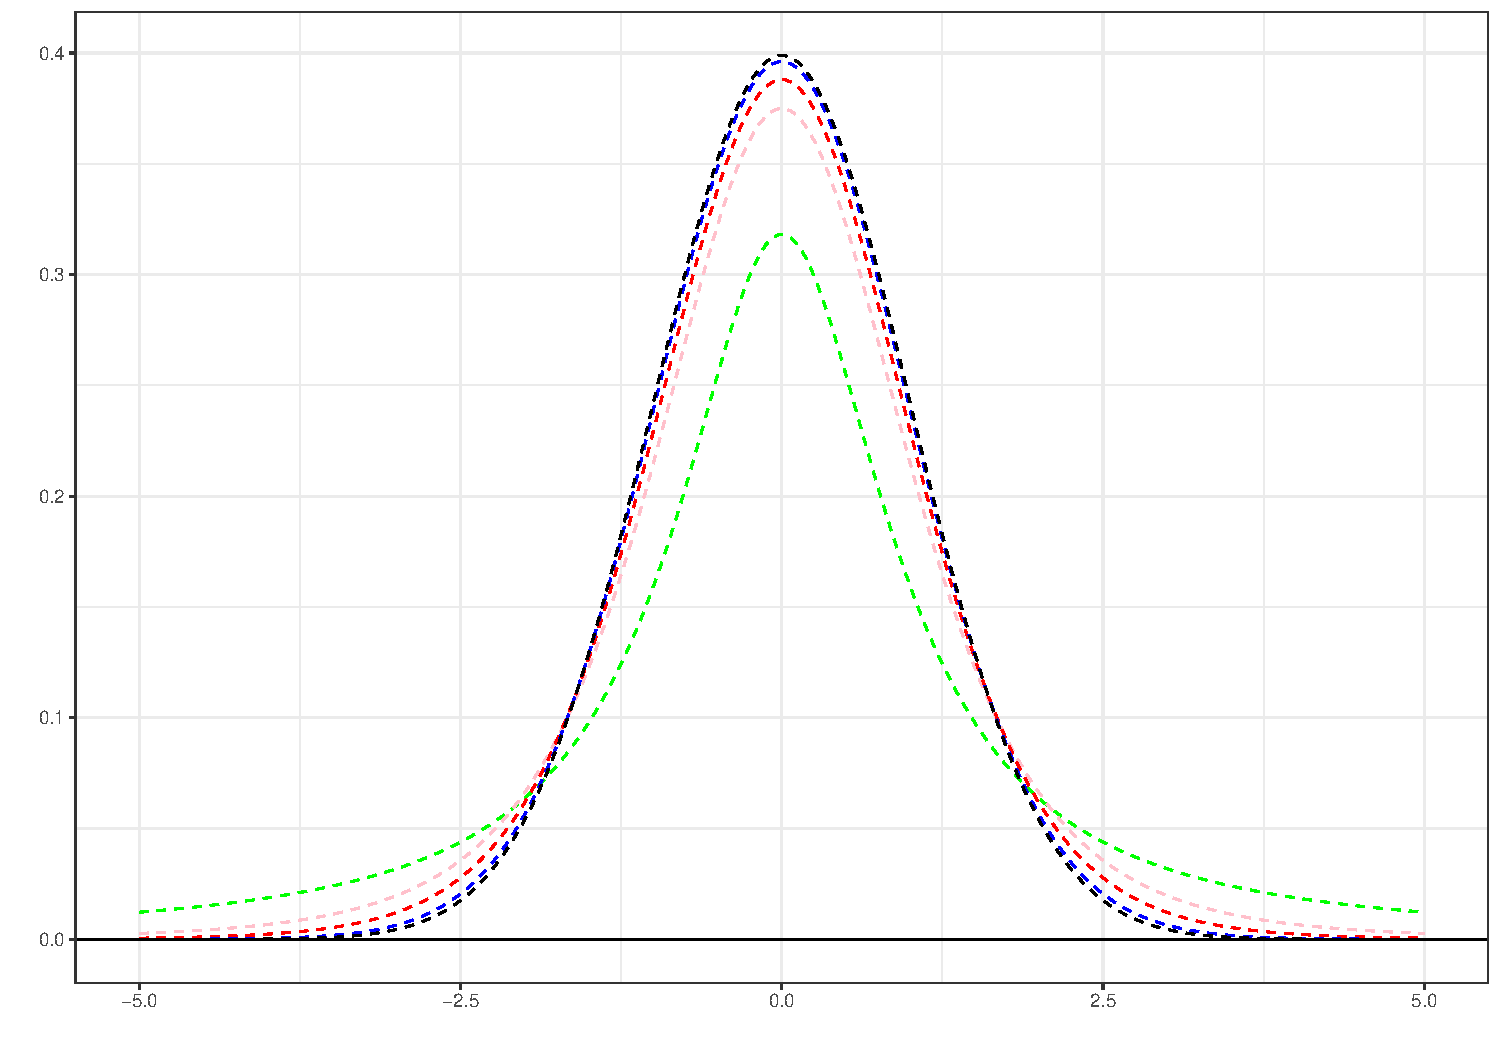
\includegraphics[width=0.6\linewidth,height=0.4\textheight]{Week10_Lect_files/figure-beamer/unnamed-chunk-55-1} \end{center}
\normalsize

\begin{itemize}
\tightlist
\item
  This distribution does have slightly longer tails than the normal
  distribution; you could never tell this from a histogram, but it is
  apparent in the normal quantile plot.
\end{itemize}
\end{frame}

\begin{frame}{Confidence intervals for a Mean, \(\sigma\) unknown}
\protect\hypertarget{confidence-intervals-for-a-mean-sigma-unknown-3}{}
\begin{itemize}
\item
  In effect, having to estimate \(\sigma\) using \(S\) adds variability.
\item
  It turns out that \[T=\frac{(\bar{X}-\mu)}{S/\sqrt{n}}\]
\end{itemize}

has a Students \(t\) distribution with \(n-1\) degrees of freedom.

\begin{itemize}
\item
  The density of a \(t\) distribution with \(k\) degrees of freedom is
  bell shaped and symmetric about 0, with heavier (longer) tails than
  that of the standard normal.

  \begin{itemize}
  \tightlist
  \item
    As \(k\) tends toward infinity, the density of the \(t\)
    distribution tends toward the density of the standard normal.
  \end{itemize}
\end{itemize}
\end{frame}

\begin{frame}[fragile]{Confidence intervals for a Mean, \(\sigma\)
unknown}
\protect\hypertarget{confidence-intervals-for-a-mean-sigma-unknown-4}{}
\tiny

\begin{Shaded}
\begin{Highlighting}[]
\FunctionTok{curve}\NormalTok{(}\FunctionTok{dnorm}\NormalTok{(x, }\DecValTok{0}\NormalTok{, }\DecValTok{1}\NormalTok{), }\SpecialCharTok{{-}}\DecValTok{4}\NormalTok{, }\DecValTok{4}\NormalTok{, }\AttributeTok{col =} \StringTok{"black"}\NormalTok{, }\AttributeTok{ylab =} \StringTok{""}\NormalTok{, }\AttributeTok{xlab =} \StringTok{""}\NormalTok{)}
\FunctionTok{curve}\NormalTok{(}\FunctionTok{dt}\NormalTok{(x, }\DecValTok{1}\NormalTok{), }\AttributeTok{add =} \ConstantTok{TRUE}\NormalTok{, }\AttributeTok{lty =} \DecValTok{2}\NormalTok{, }\AttributeTok{col =} \StringTok{"green"}\NormalTok{)}
\FunctionTok{curve}\NormalTok{(}\FunctionTok{dt}\NormalTok{(x, }\DecValTok{4}\NormalTok{), }\AttributeTok{add =} \ConstantTok{TRUE}\NormalTok{, }\AttributeTok{lty =} \DecValTok{3}\NormalTok{, }\AttributeTok{col =} \StringTok{"pink"}\NormalTok{)}
\FunctionTok{curve}\NormalTok{(}\FunctionTok{dt}\NormalTok{(x, }\DecValTok{9}\NormalTok{), }\AttributeTok{add =} \ConstantTok{TRUE}\NormalTok{, }\AttributeTok{lty =} \DecValTok{4}\NormalTok{, }\AttributeTok{col =} \StringTok{"red"}\NormalTok{)}
\FunctionTok{curve}\NormalTok{(}\FunctionTok{dt}\NormalTok{(x, }\DecValTok{36}\NormalTok{), }\AttributeTok{add =} \ConstantTok{TRUE}\NormalTok{, }\AttributeTok{lty =} \DecValTok{5}\NormalTok{, }\AttributeTok{col =} \StringTok{"blue"}\NormalTok{)}
\FunctionTok{abline}\NormalTok{(}\AttributeTok{h =} \DecValTok{0}\NormalTok{, }\AttributeTok{lwd=}\DecValTok{2}\NormalTok{)}
\FunctionTok{legend}\NormalTok{(}\StringTok{"topright"}\NormalTok{, }\AttributeTok{legend =} \FunctionTok{c}\NormalTok{(}\StringTok{"N(0, 1)"}\NormalTok{, }\StringTok{"t\_1"}\NormalTok{, }\StringTok{"t\_4"}\NormalTok{, }\StringTok{"t\_9"}\NormalTok{, }\StringTok{"t\_36"}\NormalTok{), }
       \AttributeTok{lty =} \FunctionTok{c}\NormalTok{(}\DecValTok{1}\NormalTok{, }\DecValTok{2}\NormalTok{, }\DecValTok{3}\NormalTok{, }\DecValTok{4}\NormalTok{, }\DecValTok{5}\NormalTok{), }\AttributeTok{col =}\FunctionTok{c}\NormalTok{(}\StringTok{"black"}\NormalTok{, }\StringTok{"green"}\NormalTok{, }\StringTok{"pink"}\NormalTok{, }\StringTok{"red"}\NormalTok{, }\StringTok{"blue"}\NormalTok{), }
       \AttributeTok{lwd =} \FloatTok{1.5}\NormalTok{)}
\end{Highlighting}
\end{Shaded}

\begin{center}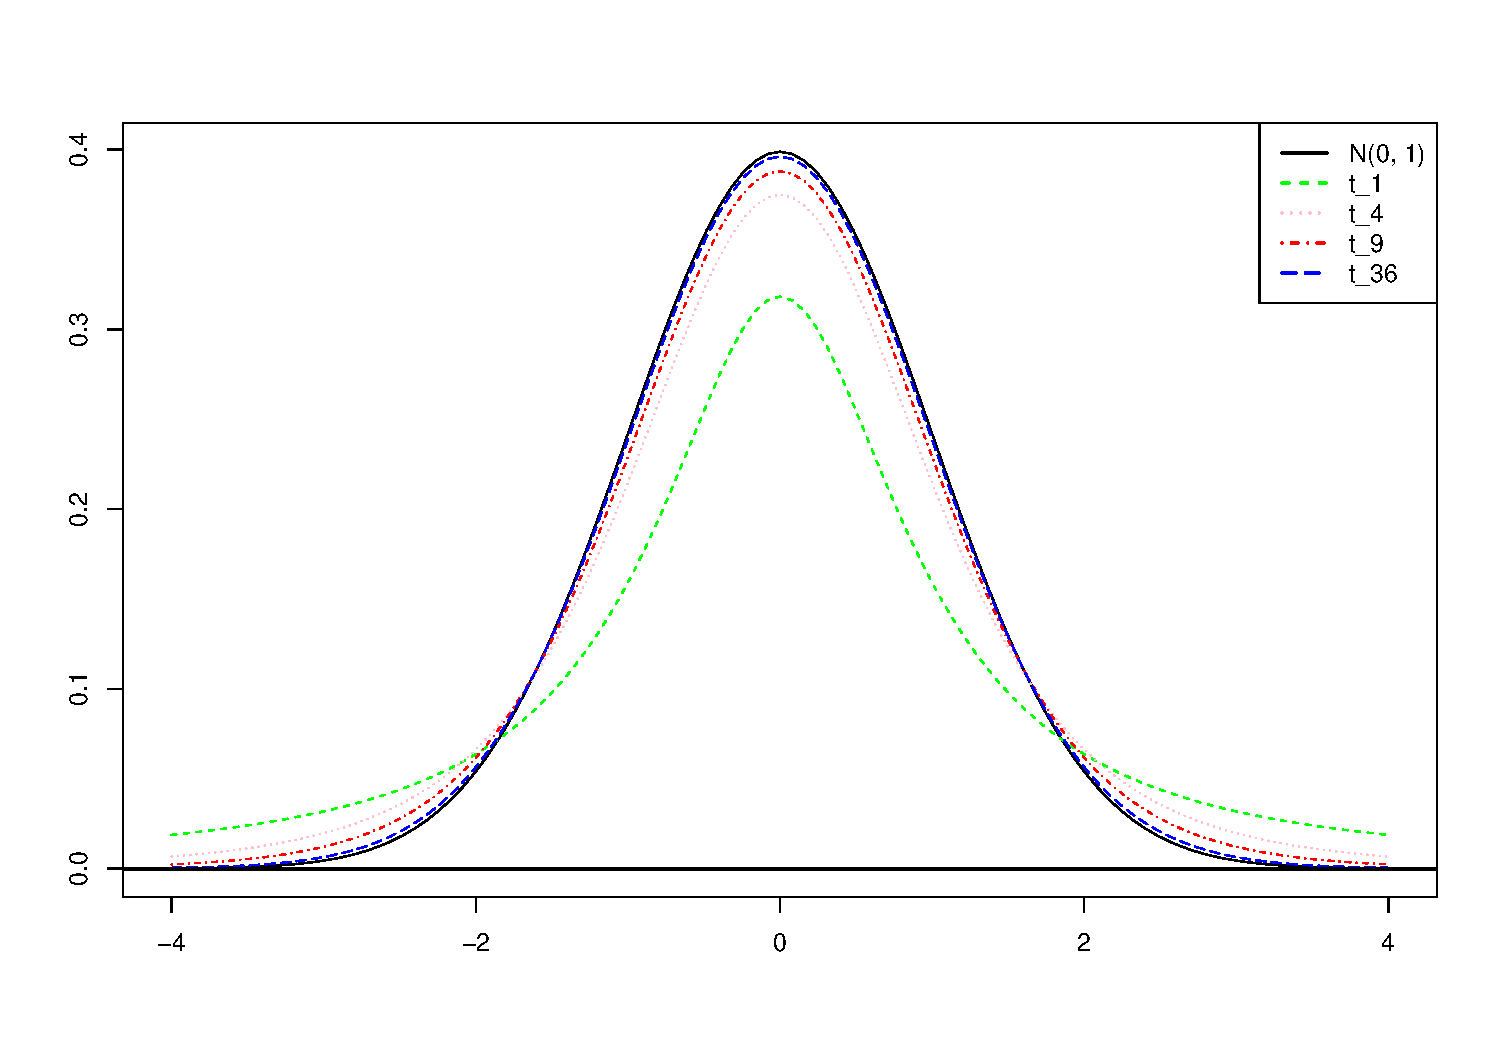
\includegraphics[width=0.6\linewidth,height=0.4\textheight]{Week10_Lect_files/figure-beamer/unnamed-chunk-56-1} \end{center}
\normalsize
\end{frame}

\begin{frame}[fragile]{Confidence intervals for a Mean, \(\sigma\)
unknown}
\protect\hypertarget{confidence-intervals-for-a-mean-sigma-unknown-5}{}
with \texttt{ggplot2}

\tiny

\begin{Shaded}
\begin{Highlighting}[]
\FunctionTok{ggplot}\NormalTok{(}\AttributeTok{data =} \FunctionTok{data.frame}\NormalTok{(}\AttributeTok{x =} \FunctionTok{c}\NormalTok{(}\SpecialCharTok{{-}}\DecValTok{5}\NormalTok{, }\DecValTok{5}\NormalTok{)), }\FunctionTok{aes}\NormalTok{(}\AttributeTok{x =}\NormalTok{ x)) }\SpecialCharTok{+} 
  \FunctionTok{theme\_bw}\NormalTok{() }\SpecialCharTok{+}
  \FunctionTok{labs}\NormalTok{(}\AttributeTok{x =} \StringTok{""}\NormalTok{, }\AttributeTok{y =} \StringTok{""}\NormalTok{) }\SpecialCharTok{+}
  \FunctionTok{stat\_function}\NormalTok{(}\AttributeTok{fun =}\NormalTok{ dt, }\AttributeTok{args =} \FunctionTok{list}\NormalTok{(}\AttributeTok{df =} \DecValTok{1}\NormalTok{), }\AttributeTok{n =} \DecValTok{200}\NormalTok{, }\AttributeTok{color =} \StringTok{"green"}\NormalTok{, }\AttributeTok{linetype =} \StringTok{"dashed"}\NormalTok{) }\SpecialCharTok{+} 
  \FunctionTok{stat\_function}\NormalTok{(}\AttributeTok{fun =}\NormalTok{ dt, }\AttributeTok{args =} \FunctionTok{list}\NormalTok{(}\AttributeTok{df =} \DecValTok{4}\NormalTok{), }\AttributeTok{n =} \DecValTok{200}\NormalTok{, }\AttributeTok{color =} \StringTok{"pink"}\NormalTok{, }\AttributeTok{linetype =} \StringTok{"dashed"}\NormalTok{) }\SpecialCharTok{+} 
  \FunctionTok{stat\_function}\NormalTok{(}\AttributeTok{fun =}\NormalTok{ dt, }\AttributeTok{args =} \FunctionTok{list}\NormalTok{(}\AttributeTok{df =} \DecValTok{9}\NormalTok{), }\AttributeTok{n =} \DecValTok{200}\NormalTok{, }\AttributeTok{color =} \StringTok{"red"}\NormalTok{, }\AttributeTok{linetype =} \StringTok{"dashed"}\NormalTok{) }\SpecialCharTok{+} 
  \FunctionTok{stat\_function}\NormalTok{(}\AttributeTok{fun =}\NormalTok{ dt, }\AttributeTok{args =} \FunctionTok{list}\NormalTok{(}\AttributeTok{df =} \DecValTok{36}\NormalTok{), }\AttributeTok{n =} \DecValTok{200}\NormalTok{, }\AttributeTok{color =} \StringTok{"blue"}\NormalTok{, }\AttributeTok{linetype =} \StringTok{"dashed"}\NormalTok{) }\SpecialCharTok{+} 
  \FunctionTok{stat\_function}\NormalTok{(}\AttributeTok{fun =}\NormalTok{ dnorm, }\AttributeTok{n =} \DecValTok{200}\NormalTok{, }\AttributeTok{color =} \StringTok{"black"}\NormalTok{, }\AttributeTok{linetype =} \StringTok{"dashed"}\NormalTok{) }\SpecialCharTok{+}
  \FunctionTok{geom\_hline}\NormalTok{(}\AttributeTok{yintercept =} \DecValTok{0}\NormalTok{)}
\end{Highlighting}
\end{Shaded}

\begin{center}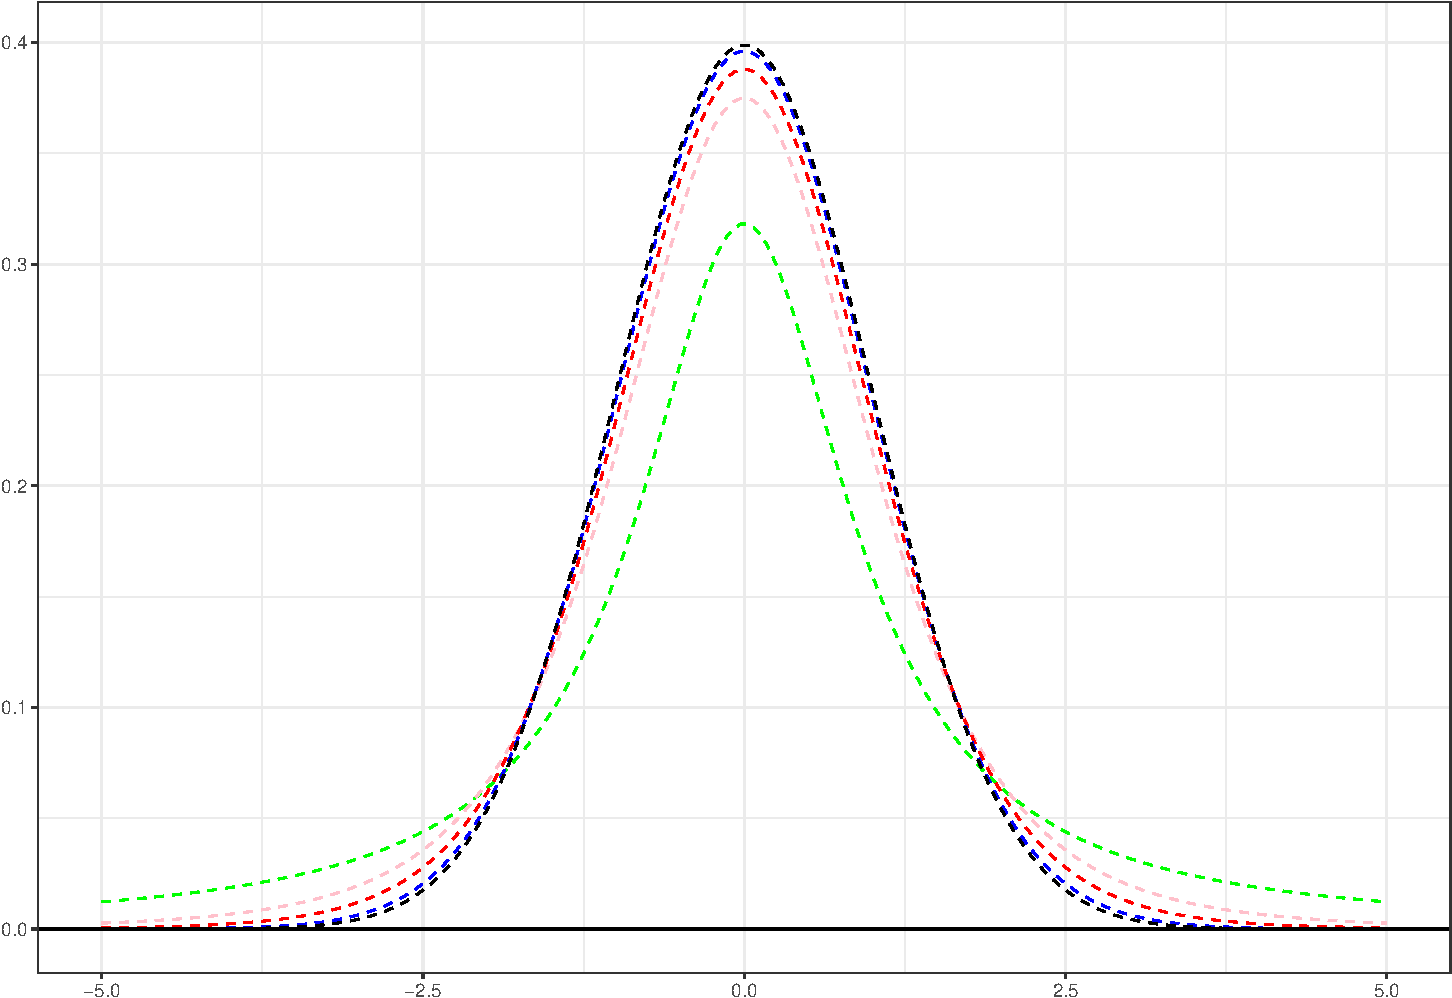
\includegraphics[width=0.6\linewidth,height=0.4\textheight]{Week10_Lect_files/figure-beamer/unnamed-chunk-57-1} \end{center}
\normalsize
\end{frame}

\begin{frame}{Confidence intervals for a Mean, \(\sigma\) unknown}
\protect\hypertarget{confidence-intervals-for-a-mean-sigma-unknown-6}{}
We derive the confidence interval for \(\mu\) when \(\sigma\) is unknown
in the same way as when \(\sigma\) is known.

\begin{itemize}
\tightlist
\item
  Let \(t_{1-\alpha/2;n-1}\) denote the \((1-\alpha/2)\) quantile of the
  \(t\) distribution with \(n-1\) degrees of freedom. Then:
  \[1-\alpha/2=P(T_{n-1}<t_{1-\alpha/2;n-1})\]
\end{itemize}

for \(0<\alpha<1\). Then using the symmetry of the \(t\) distribution,
we have: \[\begin{array}{ll}
1-\alpha&=P\left(-t_{1-\alpha/2;n-1}< \frac{\bar{X}-\mu}{S/\sqrt{n}}<t_{1-\alpha/2;n-1}\right)\\
&=P\left(\bar{X}-t_{1-\alpha/2;n-1}\times S/\sqrt{n}<\mu<\bar{X}+t_{1-\alpha/2;n-1}\times S/\sqrt{n}\right)
\end{array}\]
\end{frame}

\begin{frame}{Confidence intervals for a Mean, \(\sigma\) unknown}
\protect\hypertarget{confidence-intervals-for-a-mean-sigma-unknown-7}{}
If \(N(\mu, \sigma)\), \(i=1,\ldots, n\), with \(\sigma\) unknown then a
\((1-\alpha)\times 100\%\) confidence interval for \(\mu\) is given by:
\[\begin{array}{ll}
CI_{1-\alpha}(\mu)=P\left(\bar{X}-t_{1-\alpha/2;n-1}\times S/\sqrt{n}<\mu<\bar{X}+t_{1-\alpha/2;n-1}\times S/\sqrt{n}\right).
\end{array}\]
\end{frame}

\begin{frame}[fragile]{Example 5}
\protect\hypertarget{example-5}{}
\begin{tcolorbox}
The distribution of weights of boys in Sodor is normal with unknown mean $\mu$. From a random sample of 28 boys, we find a sample mean of 110 pounds and a sample standard deviation of 7.5 pounds. Compute a $90\%$ confidence interval. 
\end{tcolorbox}

To compute a \(90\%\) confidence interval, find the 0.95 quantile of the
\(t\) distribution with 27 degrees of freedom. That is quantile
\(t_{0.95;27}\) satisfying \(P(T_{27}<t_{0.95;27})\)

\normalsize

\begin{Shaded}
\begin{Highlighting}[]
\FunctionTok{qt}\NormalTok{(.}\DecValTok{95}\NormalTok{, }\DecValTok{27}\NormalTok{)}
\end{Highlighting}
\end{Shaded}

\begin{verbatim}
[1] 1.703288
\end{verbatim}

\normalsize
\end{frame}

\begin{frame}[fragile]{Example 5}
\protect\hypertarget{example-5-1}{}
The interval is \[\begin{array}{ll}
(110-1.7033\times 7.5/\sqrt{28},110+1.7033\times 7.5/\sqrt{28})=(107.6, 112.4).
\end{array}\]

\normalsize

\begin{Shaded}
\begin{Highlighting}[]
\CommentTok{\# Using function from PASWR2}
\FunctionTok{tsum.test}\NormalTok{(}\AttributeTok{mean.x =} \DecValTok{110}\NormalTok{, }\AttributeTok{s.x =} \FloatTok{7.5}\NormalTok{, }\AttributeTok{n.x =} \DecValTok{28}\NormalTok{, }
          \AttributeTok{conf.level =} \FloatTok{0.90}\NormalTok{)}\SpecialCharTok{$}\NormalTok{conf}
\end{Highlighting}
\end{Shaded}

\begin{verbatim}
[1] 107.5858 112.4142
attr(,"conf.level")
[1] 0.9
\end{verbatim}

\normalsize
\end{frame}

\begin{frame}[fragile]{Example 5: Birth weight of a baby}
\protect\hypertarget{example-5-birth-weight-of-a-baby}{}
\begin{tcolorbox}
The birth weight of a baby is of interest to health officials since many studies have shown possible links between this weight and conditions in later life, such as obesity or diabetes. Researchers look for possible relationships between the birth weight of a baby and age of the mother or whether or not she smokes cigarettes or drink alcohol during her pregnancy. The centers for disease control and prevention CDC, using data provided by the U.S. Department of Health and Human Services, National Center for Health Statistics, the Division of Vital Statistics as well as the CDC, maintain a database on all babies born in a given year. We will investigate different samples taken from the CDC’s database of births. Find a $99\%$ confidence interval for the mean weight of baby girls born in North Carolina in 2004.
\end{tcolorbox}

We will use the \texttt{NCBirths2004} data from the
\texttt{resampledata} package.
\end{frame}

\begin{frame}[fragile]{Example 5: Birth weight of a baby}
\protect\hypertarget{example-5-birth-weight-of-a-baby-1}{}
\normalsize

\begin{Shaded}
\begin{Highlighting}[]
\FunctionTok{library}\NormalTok{(resampledata)}
\FunctionTok{head}\NormalTok{(NCBirths2004, }\AttributeTok{n =} \DecValTok{2}\NormalTok{)}
\end{Highlighting}
\end{Shaded}

\begin{verbatim}
  ID MothersAge Tobacco Alcohol Gender Weight Gestation Smoker
1  1      30-34      No      No   Male   3827        40     No
2  2      30-34      No      No   Male   3629        38     No
\end{verbatim}

\begin{Shaded}
\begin{Highlighting}[]
\NormalTok{NCBirths2004 }\SpecialCharTok{\%\textgreater{}\%}\FunctionTok{group\_by}\NormalTok{(Gender)}\SpecialCharTok{\%\textgreater{}\%} 
  \FunctionTok{summarize}\NormalTok{(}\AttributeTok{Mean =} \FunctionTok{mean}\NormalTok{(Weight),}\AttributeTok{SD=}\FunctionTok{sd}\NormalTok{(Weight), }\AttributeTok{n =} \FunctionTok{n}\NormalTok{()) }\OtherTok{{-}\textgreater{}}\NormalTok{ BW}
\NormalTok{BW}
\end{Highlighting}
\end{Shaded}

\begin{verbatim}
# A tibble: 2 x 4
  Gender  Mean    SD     n
  <fct>  <dbl> <dbl> <int>
1 Female 3398.  486.   521
2 Male   3502.  485.   488
\end{verbatim}

\normalsize
\end{frame}

\begin{frame}[fragile]{Example 5: Birth weight of a baby}
\protect\hypertarget{example-5-birth-weight-of-a-baby-2}{}
A normal quantile plot shows that the weights are approximately normally
distributed, so \(t\) interval is reasonable. \normalsize

\begin{Shaded}
\begin{Highlighting}[]
\CommentTok{\# Using lattice}
\FunctionTok{qqmath}\NormalTok{(}\SpecialCharTok{\textasciitilde{}}\NormalTok{Weight}\SpecialCharTok{|}\NormalTok{Gender, }\AttributeTok{data =}\NormalTok{ NCBirths2004, }\AttributeTok{col =} \FunctionTok{rgb}\NormalTok{(}\DecValTok{1}\NormalTok{, }\DecValTok{0}\NormalTok{, }\DecValTok{0}\NormalTok{, }\FloatTok{0.1}\NormalTok{))}
\end{Highlighting}
\end{Shaded}

\begin{center}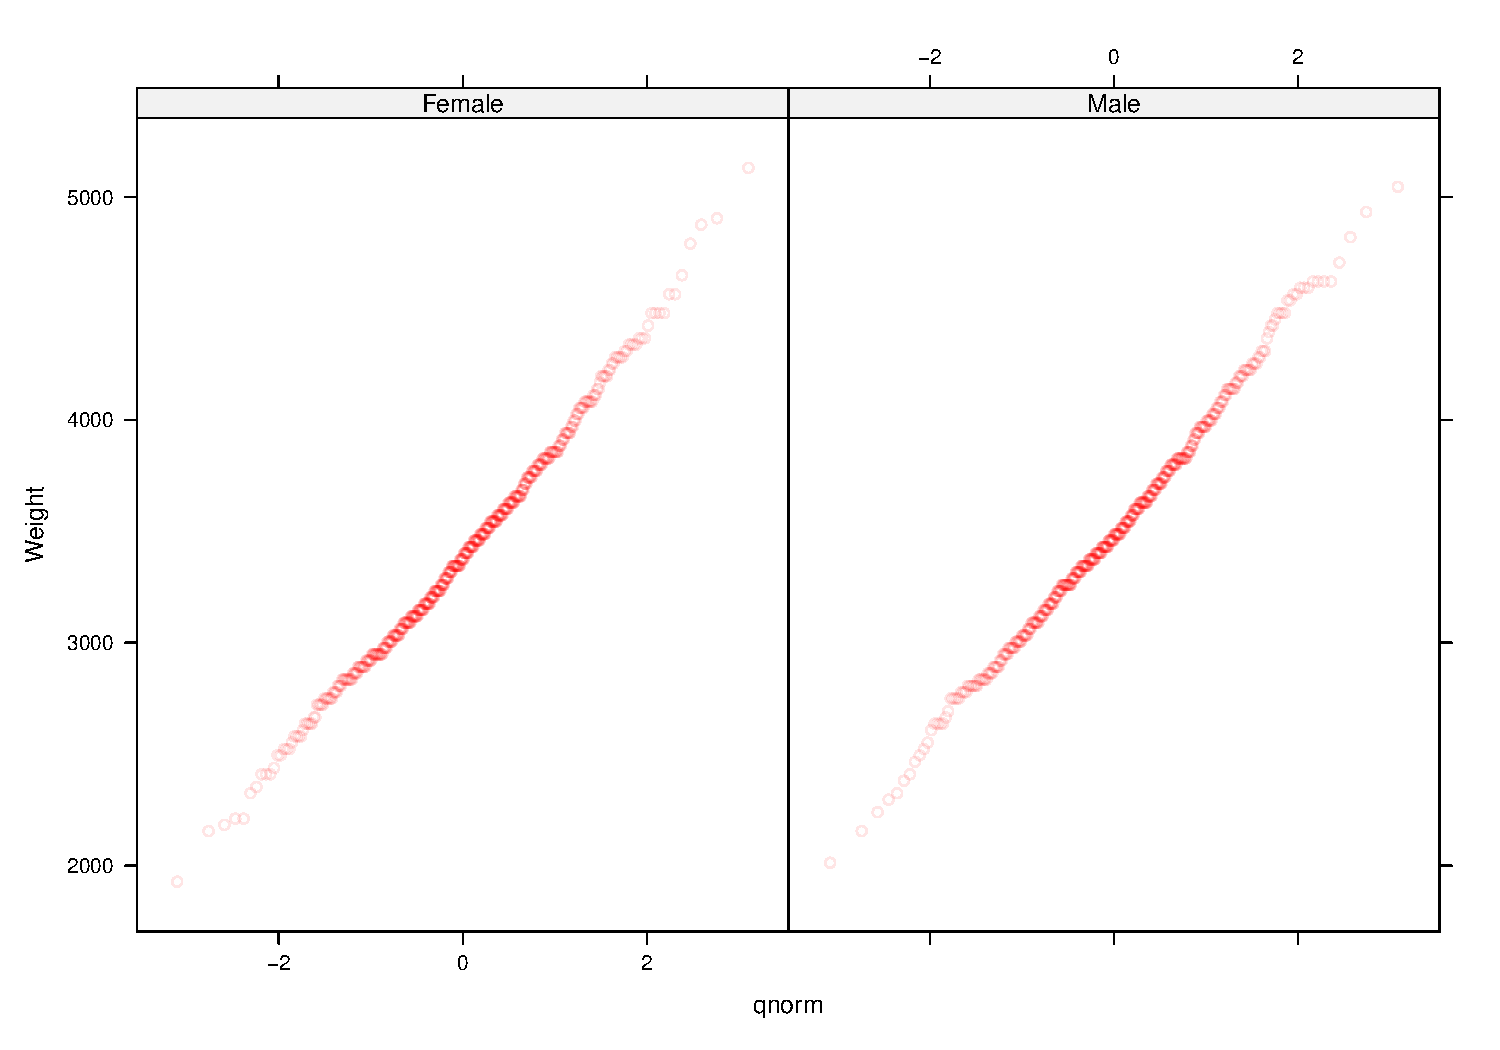
\includegraphics[width=0.7\linewidth,height=0.5\textheight]{Week10_Lect_files/figure-beamer/unnamed-chunk-61-1} \end{center}
\normalsize
\end{frame}

\begin{frame}[fragile]{Example 5: Birth weight of a baby}
\protect\hypertarget{example-5-birth-weight-of-a-baby-3}{}
\tiny

\begin{Shaded}
\begin{Highlighting}[]
\FunctionTok{ggplot}\NormalTok{(}\AttributeTok{data =}\NormalTok{ NCBirths2004, }\FunctionTok{aes}\NormalTok{(}\AttributeTok{sample =}\NormalTok{ Weight)) }\SpecialCharTok{+} 
  \FunctionTok{stat\_qq}\NormalTok{(}\AttributeTok{color =} \FunctionTok{rgb}\NormalTok{(}\DecValTok{1}\NormalTok{, }\DecValTok{0}\NormalTok{, }\DecValTok{0}\NormalTok{, }\FloatTok{0.1}\NormalTok{)) }\SpecialCharTok{+} 
  \FunctionTok{stat\_qq\_line}\NormalTok{() }\SpecialCharTok{+}
  \FunctionTok{facet\_grid}\NormalTok{(}\AttributeTok{cols =} \FunctionTok{vars}\NormalTok{(Gender)) }\SpecialCharTok{+} 
  \FunctionTok{theme\_bw}\NormalTok{()}
\end{Highlighting}
\end{Shaded}

\begin{center}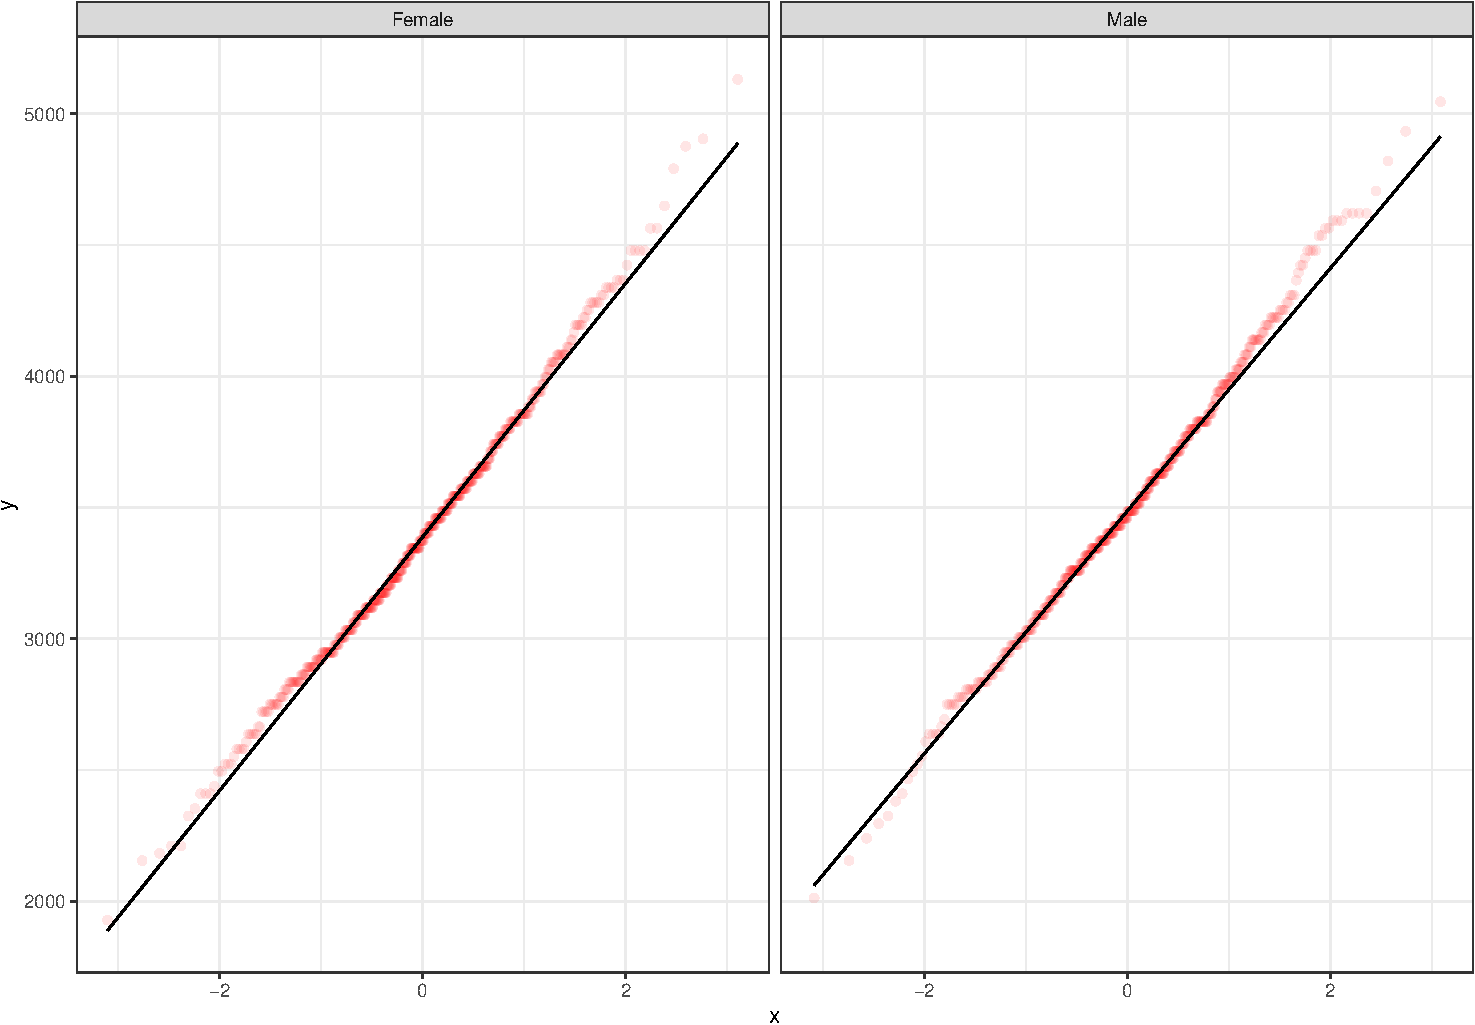
\includegraphics[width=0.7\linewidth,height=0.5\textheight]{Week10_Lect_files/figure-beamer/unnamed-chunk-62-1} \end{center}
\normalsize
\end{frame}

\begin{frame}[fragile]{Example 5: Birth weight of a baby}
\protect\hypertarget{example-5-birth-weight-of-a-baby-4}{}
Since \(1-\alpha=0.99\), then \(\alpha/2=0.005\). The 0.995 quantile for
the \(t\) distribution with 520 df, \(t_{0.995;520}\) is

\normalsize

\begin{Shaded}
\begin{Highlighting}[]
\FunctionTok{qt}\NormalTok{(}\FloatTok{0.995}\NormalTok{, }\DecValTok{520}\NormalTok{)}
\end{Highlighting}
\end{Shaded}

\begin{verbatim}
[1] 2.585317
\end{verbatim}

\normalsize

The interval is \[\begin{array}{ll}
(3398.3166987-2.585317\times 485.6911149/\sqrt{521},\\
3398.3166987+2.585317\times 485.6911149/\sqrt{521})\\
=(3343.3049953g, 3453.328402g).
\end{array}\]
\end{frame}

\begin{frame}[fragile]{Example 5: Birth weight of a baby}
\protect\hypertarget{example-5-birth-weight-of-a-baby-5}{}
\normalsize

\begin{Shaded}
\begin{Highlighting}[]
\CommentTok{\# t.test() to find confidence intervals.}
\FunctionTok{t.test}\NormalTok{(NCBirths2004}\SpecialCharTok{$}\NormalTok{Weight[NCBirths2004}\SpecialCharTok{$}\NormalTok{Gender}\SpecialCharTok{==}\StringTok{"Female"}\NormalTok{], }
       \AttributeTok{conf =} \FloatTok{0.99}\NormalTok{)}\SpecialCharTok{$}\NormalTok{conf}
\end{Highlighting}
\end{Shaded}

\begin{verbatim}
[1] 3343.305 3453.328
attr(,"conf.level")
[1] 0.99
\end{verbatim}

\begin{Shaded}
\begin{Highlighting}[]
\CommentTok{\# Or}
\NormalTok{JG }\OtherTok{\textless{}{-}}\NormalTok{ NCBirths2004 }\SpecialCharTok{\%\textgreater{}\%} 
  \FunctionTok{filter}\NormalTok{(Gender }\SpecialCharTok{==} \StringTok{"Female"}\NormalTok{) }
\FunctionTok{t.test}\NormalTok{(JG}\SpecialCharTok{$}\NormalTok{Weight, }\AttributeTok{conf =} \FloatTok{0.99}\NormalTok{)}\SpecialCharTok{$}\NormalTok{conf}
\end{Highlighting}
\end{Shaded}

\begin{verbatim}
[1] 3343.305 3453.328
attr(,"conf.level")
[1] 0.99
\end{verbatim}

\normalsize
\end{frame}

\begin{frame}[fragile]{Example 5: Birth weight of a baby}
\protect\hypertarget{example-5-birth-weight-of-a-baby-6}{}
Compare to \(99\%\) bootstrap standard error confidence intervals
\normalsize

\begin{Shaded}
\begin{Highlighting}[]
\NormalTok{girls }\OtherTok{\textless{}{-}} \FunctionTok{subset}\NormalTok{(NCBirths2004, }\AttributeTok{select =}\NormalTok{ Weight, }
                \AttributeTok{subset =}\NormalTok{ Gender }\SpecialCharTok{==}\StringTok{"Female"}\NormalTok{, }\AttributeTok{drop =} \ConstantTok{TRUE}\NormalTok{)}
\NormalTok{B }\OtherTok{\textless{}{-}} \DecValTok{10}\SpecialCharTok{\^{}}\DecValTok{4}
\NormalTok{bsmean }\OtherTok{\textless{}{-}} \FunctionTok{numeric}\NormalTok{(B)}
\ControlFlowTok{for}\NormalTok{(i }\ControlFlowTok{in} \DecValTok{1}\SpecialCharTok{:}\NormalTok{B)\{}
\NormalTok{  bss }\OtherTok{\textless{}{-}} \FunctionTok{sample}\NormalTok{(girls, }\AttributeTok{size =} \FunctionTok{length}\NormalTok{(girls), }\AttributeTok{replace =} \ConstantTok{TRUE}\NormalTok{)}
\NormalTok{  bsmean[i] }\OtherTok{\textless{}{-}} \FunctionTok{mean}\NormalTok{(bss)\}}
\NormalTok{(CIperc }\OtherTok{\textless{}{-}} \FunctionTok{quantile}\NormalTok{(bsmean, }\AttributeTok{probs =} \FunctionTok{c}\NormalTok{(}\FloatTok{0.005}\NormalTok{, }\FloatTok{0.995}\NormalTok{)))}
\end{Highlighting}
\end{Shaded}

\begin{verbatim}
    0.5%    99.5% 
3344.132 3452.721 
\end{verbatim}

\begin{Shaded}
\begin{Highlighting}[]
\NormalTok{(CIse }\OtherTok{\textless{}{-}} \FunctionTok{c}\NormalTok{(}\FunctionTok{mean}\NormalTok{(girls) }\SpecialCharTok{+} 
    \FunctionTok{c}\NormalTok{(}\SpecialCharTok{{-}}\DecValTok{1}\NormalTok{, }\DecValTok{1}\NormalTok{)}\SpecialCharTok{*}\FunctionTok{qt}\NormalTok{(.}\DecValTok{995}\NormalTok{, }\FunctionTok{length}\NormalTok{(girls) }\SpecialCharTok{{-}} \DecValTok{1}\NormalTok{)}\SpecialCharTok{*}\FunctionTok{sd}\NormalTok{(bsmean)))}
\end{Highlighting}
\end{Shaded}

\begin{verbatim}
[1] 3343.402 3453.231
\end{verbatim}

\normalsize
\end{frame}

\begin{frame}{Assumptions underlying \(t\)-confidence interval}
\protect\hypertarget{assumptions-underlying-t-confidence-interval}{}
Recall: If \(N(\mu, \sigma)\), \(i=1,\ldots, n\), with \(\sigma\)
unknown then a \((1-\alpha)\times 100\%\) confidence interval for
\(\mu\) is given by: \[\begin{array}{ll}
CI_{1-\alpha}(\mu)=P\left(\bar{X}-t_{1-\alpha/2;n-1}\times S/\sqrt{n}<\mu<\bar{X}+t_{1-\alpha/2;n-1}\times S/\sqrt{n}\right).
\end{array}\]

The \(t\) confidence interval assumes that the underlying population is
normal, so what happens if that is not the case?
\end{frame}

\begin{frame}{Assumptions underlying \(t\)-confidence interval}
\protect\hypertarget{assumptions-underlying-t-confidence-interval-1}{}
\begin{itemize}
\item
  When the population has a normal distribution, the \(t\) interval is
  exact: a \((1-\alpha)\times 100\%\) interval covers \(\mu\) with
  probability \(1-\alpha\).

  \begin{itemize}
  \tightlist
  \item
    Equivalently, misses \(\mu\) on either side with probability
    \(\alpha/2\);
  \item
    that is, the interval is completely above \(\mu\) with probability
    \(\alpha/2\) or is completely below with probability \(\alpha/2\).
  \end{itemize}
\item
  Let us check this for a non-normal population by running a simulation.
\end{itemize}
\end{frame}

\begin{frame}[fragile]{Assumptions underlying \(t\)-confidence interval}
\protect\hypertarget{assumptions-underlying-t-confidence-interval-2}{}
\begin{tcolorbox}
We draw random samples from the right-skewed gamma distribution with $\alpha=5$ and $\lambda=2$ and count the number of times the $95\%$ confidence interval misses the mean $\mu=5/2$ on each side.
\end{tcolorbox}

\normalsize

\begin{Shaded}
\begin{Highlighting}[]
\FunctionTok{set.seed}\NormalTok{(}\DecValTok{13}\NormalTok{)}
\NormalTok{x }\OtherTok{\textless{}{-}} \FunctionTok{rgamma}\NormalTok{(}\AttributeTok{n=}\DecValTok{1000}\NormalTok{, }\AttributeTok{shape=}\DecValTok{5}\NormalTok{, }\AttributeTok{rate=}\DecValTok{2}\NormalTok{)}
\CommentTok{\#create histogram to view distribution of values}
\FunctionTok{hist}\NormalTok{(x, }\AttributeTok{main=}\StringTok{""}\NormalTok{)}
\end{Highlighting}
\end{Shaded}

\begin{center}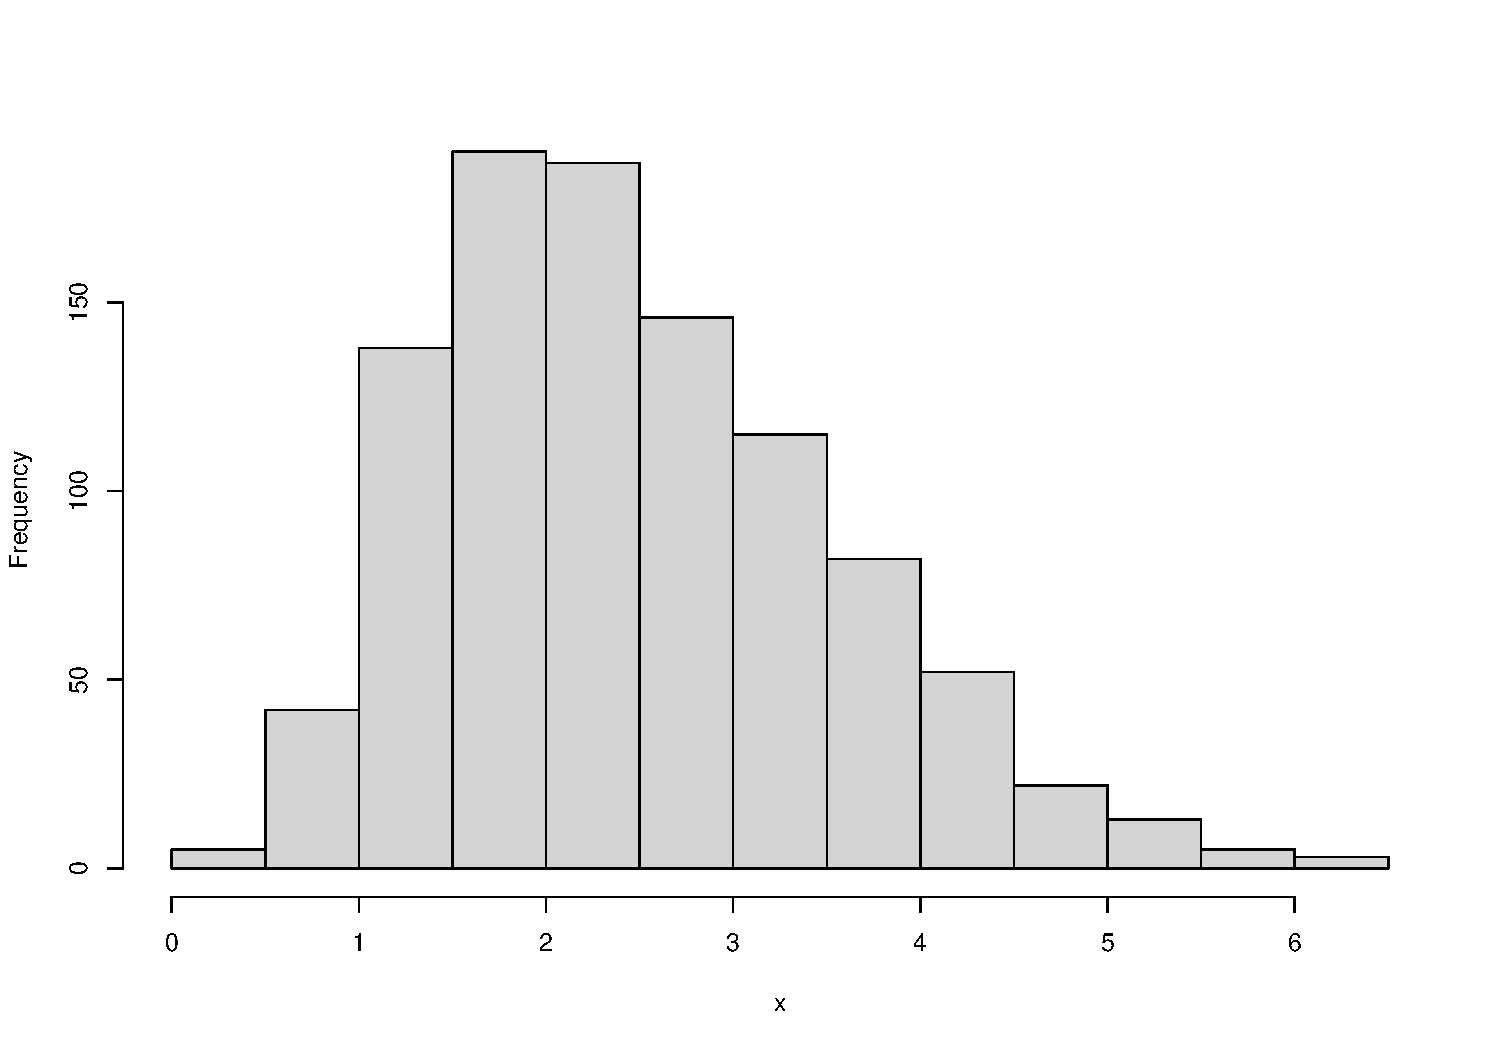
\includegraphics[width=0.6\linewidth,height=0.4\textheight]{Week10_Lect_files/figure-beamer/unnamed-chunk-66-1} \end{center}
\normalsize
\end{frame}

\begin{frame}[fragile]{Assumptions underlying \(t\)-confidence interval}
\protect\hypertarget{assumptions-underlying-t-confidence-interval-3}{}
\tiny

\begin{Shaded}
\begin{Highlighting}[]
\FunctionTok{set.seed}\NormalTok{(}\DecValTok{13}\NormalTok{)}
\NormalTok{tooLow }\OtherTok{\textless{}{-}} \DecValTok{0}       \CommentTok{\# set counter to 0}
\NormalTok{tooHigh }\OtherTok{\textless{}{-}} \DecValTok{0}      \CommentTok{\# set counter to 0}
\NormalTok{n }\OtherTok{\textless{}{-}} \DecValTok{20}           \CommentTok{\# sample size}
\NormalTok{q }\OtherTok{\textless{}{-}} \FunctionTok{qt}\NormalTok{(}\FloatTok{0.975}\NormalTok{, n }\SpecialCharTok{{-}} \DecValTok{1}\NormalTok{)}
\NormalTok{N }\OtherTok{\textless{}{-}} \DecValTok{10}\SpecialCharTok{\^{}}\DecValTok{5}
\ControlFlowTok{for}\NormalTok{(i }\ControlFlowTok{in} \DecValTok{1}\SpecialCharTok{:}\NormalTok{N)\{}
\NormalTok{  x }\OtherTok{\textless{}{-}} \FunctionTok{rgamma}\NormalTok{(n, }\AttributeTok{shape =} \DecValTok{5}\NormalTok{, }\AttributeTok{rate =} \DecValTok{2}\NormalTok{)}
\NormalTok{  xbar }\OtherTok{\textless{}{-}} \FunctionTok{mean}\NormalTok{(x)}
\NormalTok{  s }\OtherTok{\textless{}{-}} \FunctionTok{sd}\NormalTok{(x)}
\NormalTok{  L }\OtherTok{\textless{}{-}}\NormalTok{ xbar }\SpecialCharTok{{-}}\NormalTok{ q}\SpecialCharTok{*}\NormalTok{s}\SpecialCharTok{/}\FunctionTok{sqrt}\NormalTok{(n)}
\NormalTok{  U }\OtherTok{\textless{}{-}}\NormalTok{ xbar }\SpecialCharTok{+}\NormalTok{ q}\SpecialCharTok{*}\NormalTok{s}\SpecialCharTok{/}\FunctionTok{sqrt}\NormalTok{(n)}
  \ControlFlowTok{if}\NormalTok{(U }\SpecialCharTok{\textless{}} \DecValTok{5}\SpecialCharTok{/}\DecValTok{2}\NormalTok{)\{tooLow }\OtherTok{\textless{}{-}}\NormalTok{ tooLow }\SpecialCharTok{+} \DecValTok{1}\NormalTok{\}}
  \ControlFlowTok{if}\NormalTok{(L }\SpecialCharTok{\textgreater{}} \DecValTok{5}\SpecialCharTok{/}\DecValTok{2}\NormalTok{)\{tooHigh }\OtherTok{\textless{}{-}}\NormalTok{ tooHigh }\SpecialCharTok{+} \DecValTok{1}\NormalTok{\}}
\NormalTok{\}}
\NormalTok{TL }\OtherTok{\textless{}{-}}\NormalTok{ tooLow}\SpecialCharTok{/}\NormalTok{N}\SpecialCharTok{*}\DecValTok{100}
\NormalTok{TH }\OtherTok{\textless{}{-}}\NormalTok{ tooHigh}\SpecialCharTok{/}\NormalTok{N}\SpecialCharTok{*}\DecValTok{100}
\FunctionTok{c}\NormalTok{(TL, TH)}
\end{Highlighting}
\end{Shaded}

\begin{verbatim}
[1] 4.340 1.328
\end{verbatim}

\normalsize

\begin{itemize}
\item
  In one run of this simulation,

  \begin{itemize}
  \tightlist
  \item
    about \(4.34\%\) of the time, the interval was too low and below
    5/2, and
  \item
    about \(1.328\%\) of the time, the interval was too high and above
    5/2.
  \end{itemize}
\end{itemize}
\end{frame}

\begin{frame}{Assumptions underlying \(t\)-confidence interval}
\protect\hypertarget{assumptions-underlying-t-confidence-interval-4}{}
\begin{itemize}
\item
  When the population is non-normal but symmetric and the sample size is
  moderate or large, the \(t\) interval is very accurate.
\item
  The main weakness of the \(t\) confidence interval occurs when the
  population is skewed.

  \begin{itemize}
  \tightlist
  \item
    The simulation illustrated this problem.
  \end{itemize}
\item
  To see this from another point of view, we will look at the
  distributions of the \(t\) statistics,
  \[T=\frac{\bar{X}-\mu}{S/\sqrt{n}}\]
\end{itemize}

since accuracy of \(t\) intervals depends on how close the \(t\)
statistic is to having a \(t\) distribution.
\end{frame}

\begin{frame}[fragile]{Assumptions underlying \(t\)-confidence interval}
\protect\hypertarget{assumptions-underlying-t-confidence-interval-5}{}
\tiny

\begin{Shaded}
\begin{Highlighting}[]
\FunctionTok{set.seed}\NormalTok{(}\DecValTok{13}\NormalTok{); }\FunctionTok{library}\NormalTok{(gridExtra)}
\NormalTok{n }\OtherTok{\textless{}{-}} \DecValTok{10}           \CommentTok{\# sample size}
\NormalTok{q }\OtherTok{\textless{}{-}} \FunctionTok{qt}\NormalTok{(}\FloatTok{0.975}\NormalTok{, n }\SpecialCharTok{{-}} \DecValTok{1}\NormalTok{)}
\NormalTok{N }\OtherTok{\textless{}{-}} \DecValTok{10}\SpecialCharTok{\^{}}\DecValTok{5}
\NormalTok{TSU }\OtherTok{\textless{}{-}} \FunctionTok{numeric}\NormalTok{(N)}
\ControlFlowTok{for}\NormalTok{(i }\ControlFlowTok{in} \DecValTok{1}\SpecialCharTok{:}\NormalTok{N)\{}
\NormalTok{  x }\OtherTok{\textless{}{-}} \FunctionTok{runif}\NormalTok{(n, }\DecValTok{0}\NormalTok{, }\DecValTok{1}\NormalTok{)}
\NormalTok{  xbar }\OtherTok{\textless{}{-}} \FunctionTok{mean}\NormalTok{(x)}
\NormalTok{  s }\OtherTok{\textless{}{-}} \FunctionTok{sd}\NormalTok{(x)}
\NormalTok{  TSU[i] }\OtherTok{\textless{}{-}}\NormalTok{ (xbar }\SpecialCharTok{{-}} \FloatTok{0.5}\NormalTok{)}\SpecialCharTok{/}\NormalTok{(s}\SpecialCharTok{/}\FunctionTok{sqrt}\NormalTok{(n))}
\NormalTok{\}}
\NormalTok{TSE10 }\OtherTok{\textless{}{-}} \FunctionTok{numeric}\NormalTok{(N)}
\ControlFlowTok{for}\NormalTok{(i }\ControlFlowTok{in} \DecValTok{1}\SpecialCharTok{:}\NormalTok{N)\{}
\NormalTok{  x }\OtherTok{\textless{}{-}} \FunctionTok{rexp}\NormalTok{(n, }\DecValTok{1}\NormalTok{)}
\NormalTok{  xbar }\OtherTok{\textless{}{-}} \FunctionTok{mean}\NormalTok{(x)}
\NormalTok{  s }\OtherTok{\textless{}{-}} \FunctionTok{sd}\NormalTok{(x)}
\NormalTok{  TSE10[i] }\OtherTok{\textless{}{-}}\NormalTok{ (xbar }\SpecialCharTok{{-}} \DecValTok{1}\NormalTok{)}\SpecialCharTok{/}\NormalTok{(s}\SpecialCharTok{/}\FunctionTok{sqrt}\NormalTok{(n))}
\NormalTok{\}}
\NormalTok{n }\OtherTok{\textless{}{-}} \DecValTok{10}
\NormalTok{p1 }\OtherTok{\textless{}{-}} \FunctionTok{qqmath}\NormalTok{(}\SpecialCharTok{\textasciitilde{}}\NormalTok{TSU, }\AttributeTok{col =} \StringTok{"red"}\NormalTok{, }\AttributeTok{xlim =} \FunctionTok{c}\NormalTok{(}\SpecialCharTok{{-}}\DecValTok{3}\NormalTok{,}\DecValTok{3}\NormalTok{), }\AttributeTok{ylim =} \FunctionTok{c}\NormalTok{(}\SpecialCharTok{{-}}\DecValTok{3}\NormalTok{,}\DecValTok{3}\NormalTok{), }\AttributeTok{distribution =} \ControlFlowTok{function}\NormalTok{(p)\{}\FunctionTok{qt}\NormalTok{(p, }\AttributeTok{df =}\NormalTok{ n }\SpecialCharTok{{-}} \DecValTok{1}\NormalTok{)\}, }
       \AttributeTok{xlab =} \StringTok{"Theoretical t quantiles"}\NormalTok{, }\AttributeTok{ylab =} \StringTok{"Sample quantiles"}\NormalTok{, }\AttributeTok{main =} \StringTok{"Uniform, n = 10"}\NormalTok{, }
       \AttributeTok{panel =} \ControlFlowTok{function}\NormalTok{(x,...)\{}
  \FunctionTok{panel.qqmath}\NormalTok{(x, }\AttributeTok{pch =} \StringTok{"."}\NormalTok{, ...)}
  \FunctionTok{panel.abline}\NormalTok{(}\AttributeTok{a =} \DecValTok{0}\NormalTok{, }\AttributeTok{b =}\DecValTok{1}\NormalTok{, ...)\})}
\NormalTok{p2 }\OtherTok{\textless{}{-}} \FunctionTok{qqmath}\NormalTok{(}\SpecialCharTok{\textasciitilde{}}\NormalTok{TSE10, }\AttributeTok{col =} \StringTok{"red"}\NormalTok{, }\AttributeTok{xlim =} \FunctionTok{c}\NormalTok{(}\SpecialCharTok{{-}}\DecValTok{3}\NormalTok{,}\DecValTok{3}\NormalTok{), }\AttributeTok{ylim =} \FunctionTok{c}\NormalTok{(}\SpecialCharTok{{-}}\DecValTok{3}\NormalTok{,}\DecValTok{3}\NormalTok{), }\AttributeTok{distribution =} \ControlFlowTok{function}\NormalTok{(p)\{}\FunctionTok{qt}\NormalTok{(p, }\AttributeTok{df =}\NormalTok{ n }\SpecialCharTok{{-}} \DecValTok{1}\NormalTok{)\}, }
       \AttributeTok{xlab =} \StringTok{"Theoretical t quantiles"}\NormalTok{, }\AttributeTok{ylab =} \StringTok{"Sample quantiles"}\NormalTok{, }\AttributeTok{main =} \StringTok{"Exponential, n = 10"}\NormalTok{, }
       \AttributeTok{panel =} \ControlFlowTok{function}\NormalTok{(x,...)\{}
  \FunctionTok{panel.qqmath}\NormalTok{(x, }\AttributeTok{pch =} \StringTok{"."}\NormalTok{, ...)}
  \FunctionTok{panel.abline}\NormalTok{(}\AttributeTok{a =} \DecValTok{0}\NormalTok{, }\AttributeTok{b =} \DecValTok{1}\NormalTok{, ...)\})}
\NormalTok{gridExtra}\SpecialCharTok{::}\FunctionTok{grid.arrange}\NormalTok{(p1, p2, }\AttributeTok{ncol =} \DecValTok{2}\NormalTok{)}
\end{Highlighting}
\end{Shaded}

\normalsize
\end{frame}

\begin{frame}{Assumptions underlying \(t\)-confidence interval}
\protect\hypertarget{assumptions-underlying-t-confidence-interval-6}{}
\tiny

\begin{center}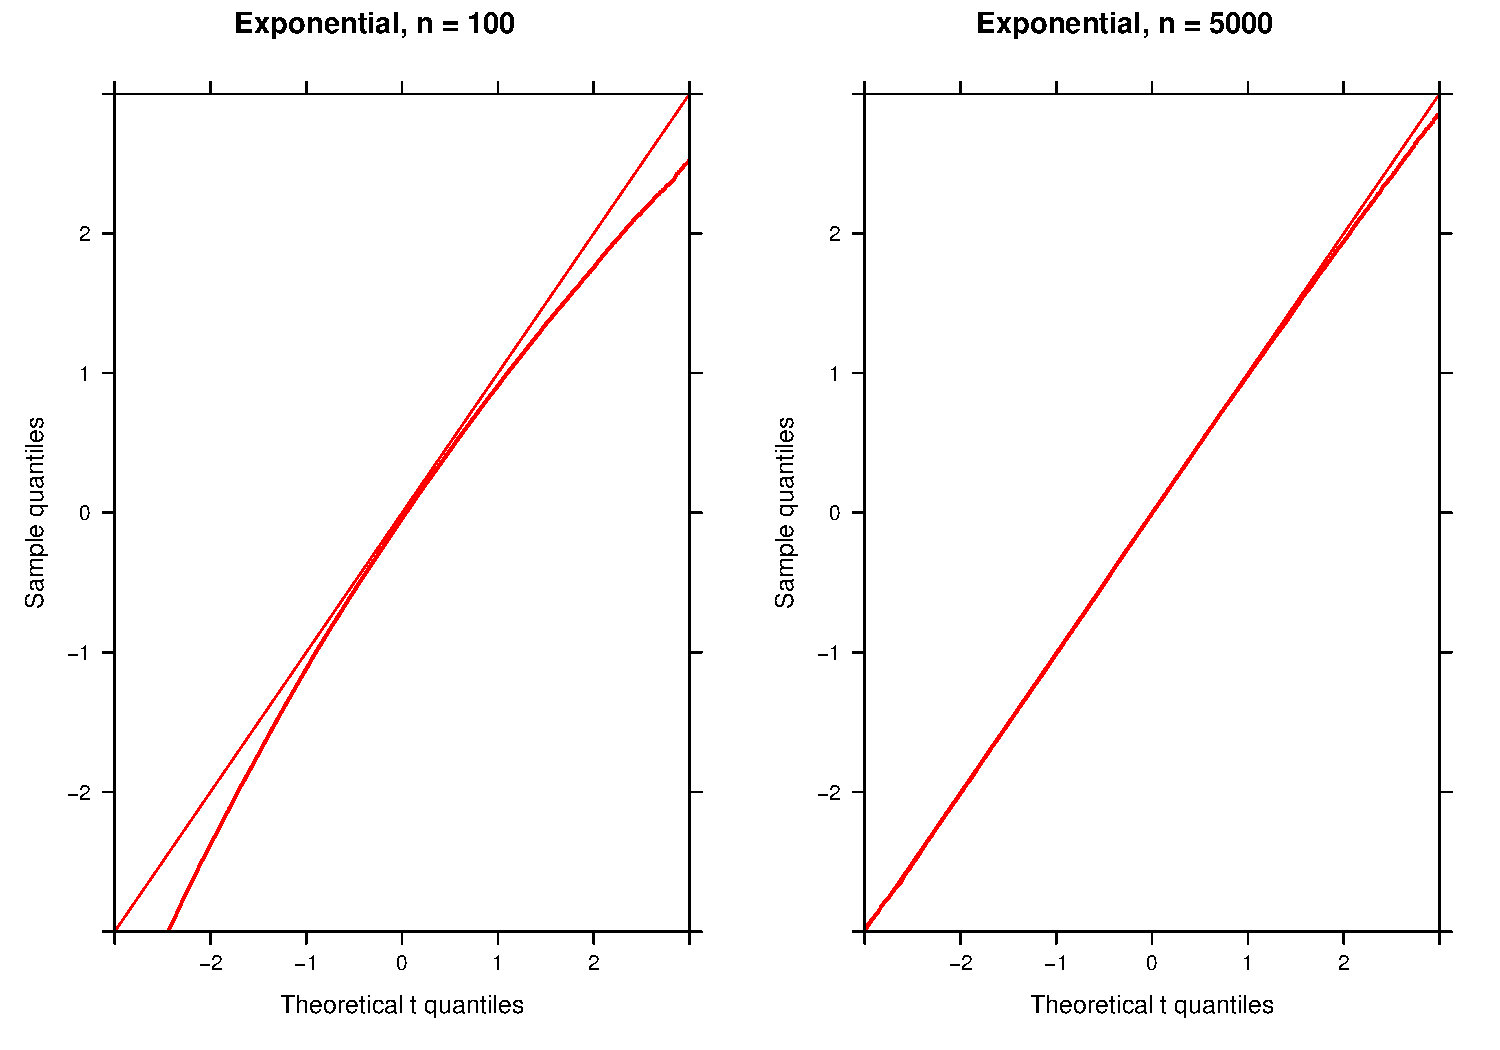
\includegraphics[width=0.8\linewidth,height=0.5\textheight]{Week10_Lect_files/figure-beamer/unnamed-chunk-69-1} \end{center}
\normalsize

\begin{itemize}
\item
  Notice that for the uniform population, the distribution of the \(t\)
  statistic is close to the \(t\) distribution, except in the tails.
\item
  For exponential populations, the discrepancy is much larger, and the
  discrepancy decreases only slowly as the sample size increases.
\end{itemize}
\end{frame}

\begin{frame}[fragile]{Assumptions underlying \(t\)-confidence interval}
\protect\hypertarget{assumptions-underlying-t-confidence-interval-7}{}
\tiny

\begin{Shaded}
\begin{Highlighting}[]
\FunctionTok{set.seed}\NormalTok{(}\DecValTok{13}\NormalTok{); }\FunctionTok{library}\NormalTok{(gridExtra)}
\NormalTok{n }\OtherTok{\textless{}{-}} \DecValTok{10}           \CommentTok{\# sample size}
\NormalTok{q }\OtherTok{\textless{}{-}} \FunctionTok{qt}\NormalTok{(}\FloatTok{0.975}\NormalTok{, n }\SpecialCharTok{{-}} \DecValTok{1}\NormalTok{)}
\NormalTok{N }\OtherTok{\textless{}{-}} \DecValTok{10}\SpecialCharTok{\^{}}\DecValTok{5}
\NormalTok{n }\OtherTok{\textless{}{-}} \DecValTok{100}
\NormalTok{TSE100 }\OtherTok{\textless{}{-}} \FunctionTok{numeric}\NormalTok{(N)}
\ControlFlowTok{for}\NormalTok{(i }\ControlFlowTok{in} \DecValTok{1}\SpecialCharTok{:}\NormalTok{N)\{}
\NormalTok{  x }\OtherTok{\textless{}{-}} \FunctionTok{rexp}\NormalTok{(n, }\DecValTok{1}\NormalTok{)}
\NormalTok{  xbar }\OtherTok{\textless{}{-}} \FunctionTok{mean}\NormalTok{(x)}
\NormalTok{  s }\OtherTok{\textless{}{-}} \FunctionTok{sd}\NormalTok{(x)}
\NormalTok{  TSE100[i] }\OtherTok{\textless{}{-}}\NormalTok{ (xbar }\SpecialCharTok{{-}} \DecValTok{1}\NormalTok{)}\SpecialCharTok{/}\NormalTok{(s}\SpecialCharTok{/}\FunctionTok{sqrt}\NormalTok{(n))\}}
\NormalTok{n }\OtherTok{\textless{}{-}} \DecValTok{5000}
\NormalTok{TSE5000 }\OtherTok{\textless{}{-}} \FunctionTok{numeric}\NormalTok{(N)}
\ControlFlowTok{for}\NormalTok{(i }\ControlFlowTok{in} \DecValTok{1}\SpecialCharTok{:}\NormalTok{N)\{}
\NormalTok{  x }\OtherTok{\textless{}{-}} \FunctionTok{rexp}\NormalTok{(n, }\DecValTok{1}\NormalTok{)}
\NormalTok{  xbar }\OtherTok{\textless{}{-}} \FunctionTok{mean}\NormalTok{(x)}
\NormalTok{  s }\OtherTok{\textless{}{-}} \FunctionTok{sd}\NormalTok{(x)}
\NormalTok{  TSE5000[i] }\OtherTok{\textless{}{-}}\NormalTok{ (xbar }\SpecialCharTok{{-}} \DecValTok{1}\NormalTok{)}\SpecialCharTok{/}\NormalTok{(s}\SpecialCharTok{/}\FunctionTok{sqrt}\NormalTok{(n))\}}
\NormalTok{n }\OtherTok{\textless{}{-}} \DecValTok{100}
\NormalTok{p1}\OtherTok{\textless{}{-}}\FunctionTok{qqmath}\NormalTok{(}\SpecialCharTok{\textasciitilde{}}\NormalTok{TSE100,}\AttributeTok{col =} \StringTok{"red"}\NormalTok{, }\AttributeTok{xlim =} \FunctionTok{c}\NormalTok{(}\SpecialCharTok{{-}}\DecValTok{3}\NormalTok{,}\DecValTok{3}\NormalTok{), }\AttributeTok{ylim =} \FunctionTok{c}\NormalTok{(}\SpecialCharTok{{-}}\DecValTok{3}\NormalTok{,}\DecValTok{3}\NormalTok{), }\AttributeTok{distribution =} \ControlFlowTok{function}\NormalTok{(p)\{}\FunctionTok{qt}\NormalTok{(p, }\AttributeTok{df =}\NormalTok{ n }\SpecialCharTok{{-}} \DecValTok{1}\NormalTok{)\}, }
       \AttributeTok{xlab =} \StringTok{"Theoretical t quantiles"}\NormalTok{, }\AttributeTok{ylab =} \StringTok{"Sample quantiles"}\NormalTok{, }\AttributeTok{main =} \StringTok{"Exponential, n = 100"}\NormalTok{, }
       \AttributeTok{panel =} \ControlFlowTok{function}\NormalTok{(x,...)\{}
  \FunctionTok{panel.qqmath}\NormalTok{(x, }\AttributeTok{pch =} \StringTok{"."}\NormalTok{, ...)}
  \FunctionTok{panel.abline}\NormalTok{(}\AttributeTok{a =} \DecValTok{0}\NormalTok{, }\AttributeTok{b =} \DecValTok{1}\NormalTok{, ...)\})}
\NormalTok{n }\OtherTok{\textless{}{-}} \DecValTok{100}
\NormalTok{p2}\OtherTok{\textless{}{-}}\FunctionTok{qqmath}\NormalTok{(}\SpecialCharTok{\textasciitilde{}}\NormalTok{TSE5000,}\AttributeTok{col =} \StringTok{"red"}\NormalTok{, }\AttributeTok{xlim =} \FunctionTok{c}\NormalTok{(}\SpecialCharTok{{-}}\DecValTok{3}\NormalTok{,}\DecValTok{3}\NormalTok{), }\AttributeTok{ylim =} \FunctionTok{c}\NormalTok{(}\SpecialCharTok{{-}}\DecValTok{3}\NormalTok{,}\DecValTok{3}\NormalTok{), }\AttributeTok{distribution =} \ControlFlowTok{function}\NormalTok{(p)\{}\FunctionTok{qt}\NormalTok{(p, }\AttributeTok{df =}\NormalTok{ n }\SpecialCharTok{{-}} \DecValTok{1}\NormalTok{)\}, }
       \AttributeTok{xlab =} \StringTok{"Theoretical t quantiles"}\NormalTok{, }\AttributeTok{ylab =} \StringTok{"Sample quantiles"}\NormalTok{, }\AttributeTok{main =} \StringTok{"Exponential, n = 5000"}\NormalTok{, }
       \AttributeTok{panel =} \ControlFlowTok{function}\NormalTok{(x,...)\{}
  \FunctionTok{panel.qqmath}\NormalTok{(x, }\AttributeTok{pch =} \StringTok{"."}\NormalTok{, ...)}
  \FunctionTok{panel.abline}\NormalTok{(}\AttributeTok{a =} \DecValTok{0}\NormalTok{, }\AttributeTok{b =} \DecValTok{1}\NormalTok{, ...)\})}
\NormalTok{gridExtra}\SpecialCharTok{::}\FunctionTok{grid.arrange}\NormalTok{(p1, p2, }\AttributeTok{ncol =} \DecValTok{2}\NormalTok{)}
\end{Highlighting}
\end{Shaded}

\normalsize
\end{frame}

\begin{frame}{Assumptions underlying \(t\)-confidence interval}
\protect\hypertarget{assumptions-underlying-t-confidence-interval-8}{}
\tiny

\begin{center}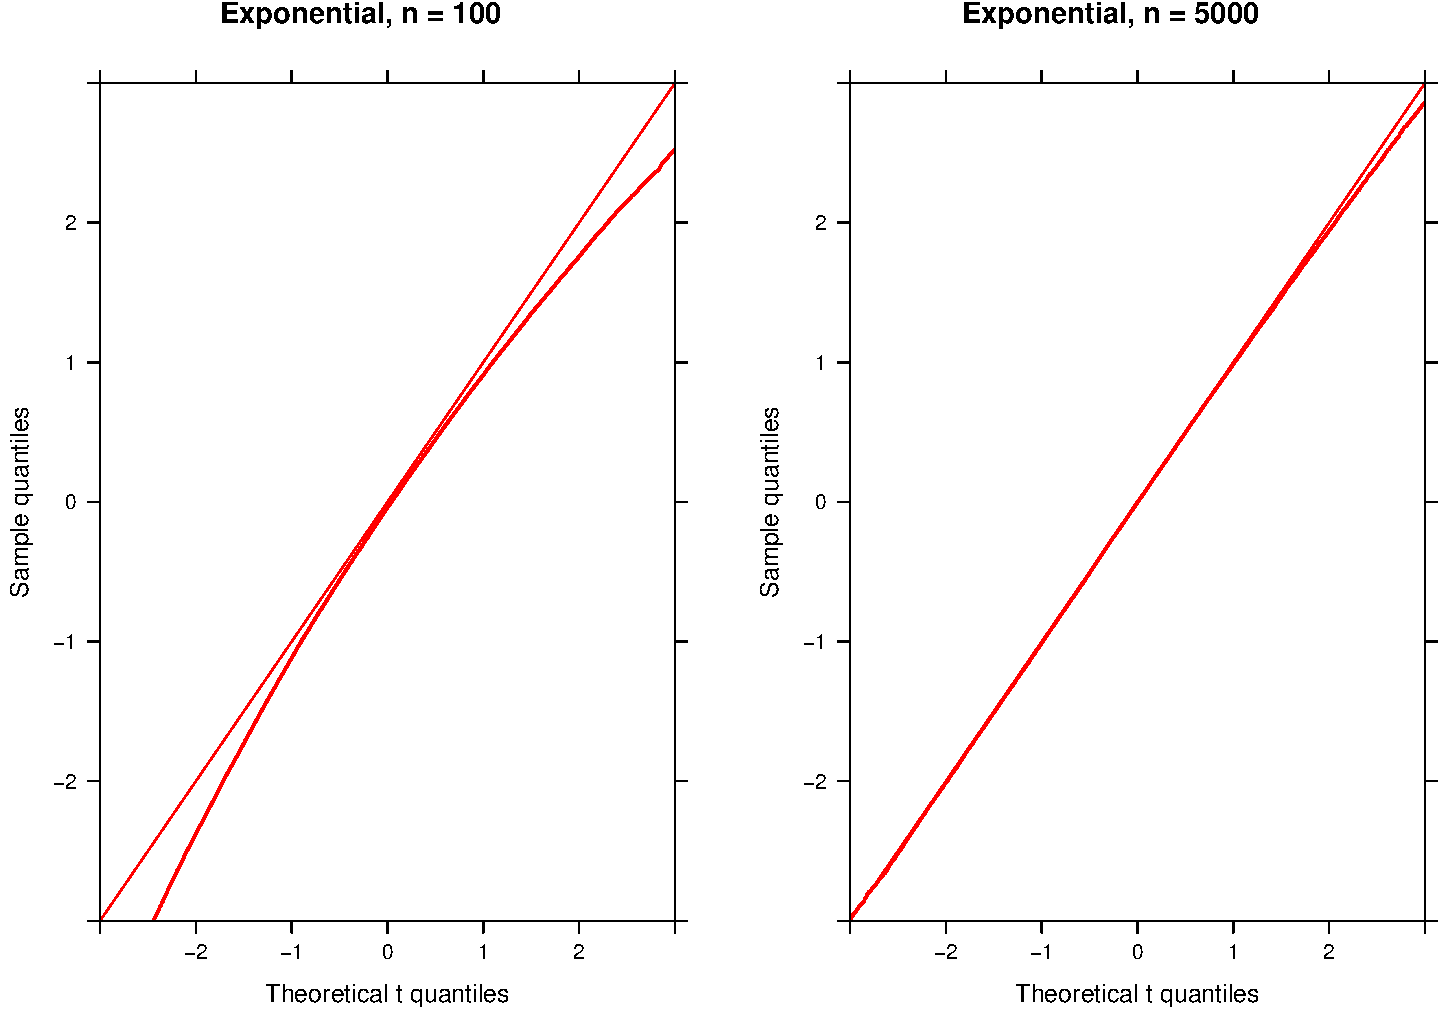
\includegraphics[width=0.8\linewidth,height=0.5\textheight]{Week10_Lect_files/figure-beamer/unnamed-chunk-71-1} \end{center}
\normalsize

\begin{itemize}
\tightlist
\item
  For an exponential population, we must have \(n>5000\)
\end{itemize}
\end{frame}

\begin{frame}{Assumptions underlying \(t\)-confidence interval}
\protect\hypertarget{assumptions-underlying-t-confidence-interval-9}{}
\begin{itemize}
\item
  Before using a \(t\) confidence interval, you should create a normal
  quantile plot to see whether the data are skewed.
\item
  The larger the sample size, the more skew can be tolerated.
\item
  However, be particularly careful with outliers: since \(\bar{x}\) is
  sensitive to extreme values;

  \begin{itemize}
  \tightlist
  \item
    If the outliers cannot be removed, then advanced, more robust
    techniques may be required.
  \end{itemize}
\end{itemize}
\end{frame}

\end{document}
